
%%%%%%%%%%%%%%%%%%%%%%%%%%%%%%%%%%%%%%%%%%%%%%%%%%%%%%
% A Beamer template for University of Sussex
% Based on THU beamer theme
% Author: Tomoto Masuda                  
% Date: Sep 2024                            
%%%%%%%%%%%%%%%%%%%%%%%%%%%%%%%%%%%%%%%%%%%%

\documentclass[serif, aspectratio=169]{beamer}
%\documentclass[serif]{beamer}  % for 4:3 ratio

%%%%%%%%%%%%%%%%%%%%%%%%%%%%%%%%%%%%%%%%%%%%%
% 複数のアペンディックスリンクを右下に配置するコマンドを定義
\newcommand{\employmenttypelinks}{%
    \vfill % 下部に押し下げる
    \hfill % 右寄せ
    {\small % ボタンのフォントサイズを小さくする
        \hyperlink{appendix1}{\beamerbutton{Full ver}} \,
        \hyperlink{appendix2}{\beamerbutton{By industry}} \,
        \hyperlink{workers_number}{\beamerbutton{Number of workers}}
    }
}
%%%%%%%%%%%%%%%%%%%%%%%%%%%%%%%%%%%%%%%%%%%%%
\newcommand{\gendergaplinks}{%
    \vfill % 下部に押し下げる
    \hfill % 右寄せ
    {\small % ボタンのフォントサイズを小さくする
        \hyperlink{gendergapindex}{\beamerbutton{Reference}} \,

    }
}
%%%%%%%%%%%%%%%%%%%%%%%%%%%%%%%%%%%%%%%%%%%%%

\newcommand{\unemploymentinsurancelinks}{%
    \vfill % 下部に押し下げる
    \hfill % 右寄せ
    {\small % ボタンのフォントサイズを小さくする
        \hyperlink{unemploymentinsurance}{\beamerbutton{Reference}} \,

    }
}
%%%%%%%%%%%%%%%%%%%%%%%%%%%%%%%%%%%%%%%%%%%%%
\newcommand{\incomebandlinks}{%
    \vfill % 下部に押し下げる
    \hfill % 右寄せ
    {\small % ボタンのフォントサイズを小さくする
        \hyperlink{income_band}{\beamerbutton{Reference}} \,

    }
}
%%%%%%%%%%%%%%%%%%%%%%%%%%%%%%%%%%%%%%%%%%%%
\newcommand{\longtermimpactlinks}{%
    \vfill % 下部に押し下げる
    \hfill % 右寄せ
    {\small % ボタンのフォントサイズを小さくする
        \hyperlink{real_GDP_growth_rate}{\beamerbutton{GRP}} \,
        \hyperlink{short_term_unemployment}{\beamerbutton{Unemp}} \,

    }
}
%%%%%%%%%%%%%%%%%%%%%%%%%%%%%%%%%%%%%%%%%%%%
\newcommand{\numbersofworkerslinks}{%
    \vfill % 下部に押し下げる
    \hfill % 右寄せ
    {\small % ボタンのフォントサイズを小さくする
        \hyperlink{numbers_of_workers_full}{\beamerbutton{Full ver}} \,
        \hyperlink{appendix3}{\beamerbutton{Gender proportion by industry}} \,
        \hyperlink{outmigration}{\beamerbutton{Number of net migration}} \,
    }
}
%%%%%%%%%%%%%%%%%%%%%%%%%%%%%%%%%%%%%%%%%%%%%

%%%%%%%%%%%%%%%%%%%%%%%%%%%%%%%%%%%%%%%%%%%%%
% 複数のアペンディックスリンクを右下に配置するコマンドを定義
\newcommand{\literaturelinks}{%
    \vfill % 下部に押し下げる
    \hfill % 右寄せ
    {\small % ボタンのフォントサイズを小さくする
        \hyperlink{risk_adjustment_hypothesis}{\beamerbutton{Reference1}} \,
        \hyperlink{shock_coping_strategy}{\beamerbutton{Reference2}} \,
        \hyperlink{theoretical_perspective}{\beamerbutton{Reference3}} \,
    }
}
%%%%%%%%%%%%%%%%%%%%%%%%%%%%%%%%%%%%%%%%%%%%%

\newcommand{\datalinks}{%
    \vfill % 下部に押し下げる
    \hfill % 右寄せ
    {\small % ボタンのフォントサイズを小さくする
        \hyperlink{data_full}{\beamerbutton{Reference}} \,

    }
}
%%%%%%%%%%%%%%%%%%%%%%%%%%%%%%%%%%%%%%%%%%%%

\newcommand{\workersinks}{%
    \vfill % 下部に押し下げる
    \hfill % 右寄せ
    {\small % ボタンのフォントサイズを小さくする
        \hyperlink{workers_number}{\beamerbutton{→ Number of workers}} \,

    }
}
%%%%%%%%%%%%%%%%%%%%%%%%%%%%%%%%%%%%%%%%%%%%
%%%%%%%%%%%%%%%%%%%%%%%%%%%%%%%%%%%%%%%%%%%%
\newcommand{\conclusionlinks}{%
    \vfill % 下部に押し下げる
    \hfill % 右寄せ
    {\small % ボタンのフォントサイズを小さくする
        \hyperlink{workers_number}{\beamerbutton{Number of workers}} \,
        \hyperlink{outmigration}{\beamerbutton{Outmigration}} \,
        \hyperlink{event_study_results}{\beamerbutton{GRP}} \,
        \hyperlink{image}{\beamerbutton{Image}} \,
        \hyperlink{LFP}{\beamerbutton{LFP}} \,
        \hyperlink{did}{\beamerbutton{DID}} \,

    }
}
%%%%%%%%%%%%%%%%%%%%%%%%%%%%%%%%%%%%%%%%%%%%
%%%%%%%%%%%%%%%%%%%%%%%%%%%%%%%%%%%%%%%%%%%%%

\newcommand{\occupatiolinks}{%
    \vfill % 下部に押し下げる
    \hfill % 右寄せ
    {\small % ボタンのフォントサイズを小さくする
        \hyperlink{appendix1}{\beamerbutton{Reference}} \,
    }
}
%%%%%%%%%%%%%%%%%%%%%%%%%%%%%%%%%%%%%%%%%%%%%
%%%%%%%%%%%%%%%%%%%%%%%%%%%%%%%%%%%%%%%%%%%%%

\newcommand{\evacueeslinks}{%
    \vfill % 下部に押し下げる
    \hfill % 右寄せ
    {\small % ボタンのフォントサイズを小さくする
        \hyperlink{evacuees_main}{\beamerbutton{→ Number of Evacuees}} \,
    }
}
%%%%%%%%%%%%%%%%%%%%%%%%%%%%%%%%%%%%%%%%%%%%%
%%%%%%%%%%%%%%%%%%%%%%%%%%%%%%%%%%%%%%%%%%%%%

\newcommand{\regularlinks}{%
    \vfill % 下部に押し下げる
    \hfill % 右寄せ
    {\small % ボタンのフォントサイズを小さくする
        \hyperlink{regular_placebo}{\beamerbutton{Placebo test}} \,
    }
}
%%%%%%%%%%%%%%%%%%%%%%%%%%%%%%%%%%%%%%%%%%%%%
%%%%%%%%%%%%%%%%%%%%%%%%%%%%%%%%%%%%%%%%%%%%%

\newcommand{\nonregularlinks}{%
    \vfill % 下部に押し下げる
    \hfill % 右寄せ
    {\small % ボタンのフォントサイズを小さくする
        \hyperlink{nonregular_placebo}{\beamerbutton{Placebo test}} \,
    }
}
%%%%%%%%%%%%%%%%%%%%%%%%%%%%%%%%%%%%%%%%%%%%%
%%%%%%%%%%%%%%%%%%%%%%%%%%%%%%%%%%%%%%%%%%%%%

\newcommand{\employmentprobabilitylinks}{%
    \vfill % 下部に押し下げる
    \hfill % 右寄せ
    {\small % ボタンのフォントサイズを小さくする
        \hyperlink{employed_placebo}{\beamerbutton{Placebo test}} \,
    }
}
%%%%%%%%%%%%%%%%%%%%%%%%%%%%%%%%%%%%%%%%%%%%%
%%%%%%%%%%%%%%%%%%%%%%%%%%%%%%%%%%%%%%%%%%%%%

\newcommand{\differentemploymenttypeslinks}{%
    \vfill % 下部に押し下げる
    \hfill % 右寄せ
    {\small % ボタンのフォントサイズを小さくする
        \hyperlink{proportion_of_employment_type}{\beamerbutton{Proportion of employment types}} \,
        \hyperlink{different_types_placebo}{\beamerbutton{Placebo test}} \,
    }
}
%%%%%%%%%%%%%%%%%%%%%%%%%%%%%%%%%%%%%%%%%%%%%

%%%%%%%%%%%%%%%%%%%%%%%%%%%%%%%%%%%%%%%%%%%%%

\newcommand{\eventstudyongrplinks}{%
    \vfill % 下部に押し下げる
    \hfill % 右寄せ
    {\small % ボタンのフォントサイズを小さくする
        \hyperlink{event_study_results}{\beamerbutton{this case}} \,
    }
}
%%%%%%%%%%%%%%%%%%%%%%%%%%%%%%%%%%%%%%%%%%%%%

% ボタンスタイルのカスタマイズ
\setbeamertemplate{navigation symbols}{}  % ナビゲーションシンボルを非表示
\setbeamercolor{button}{bg=gray!15,fg=black}  % ボタンの色を設定

% カスタム「戻る」ボタンコマンドの定義
\newcommand{\returnbutton}[2]{%
  \vspace{-1.0cm}  % 上部の余白を調整
  \hfill  % 右寄せ
  \hyperlink{#1}{%
    {\footnotesize\beamerbutton{#2}}%
  }%
  \vspace{0.3cm}  % ボタン下の余白
}

%%%%%%%%%%%%%%%%%%%%%%%%%%%%%%%%%%%%%%%%%%%%%

\usepackage{adjustbox}   % 表のサイズ調整のため

\usepackage[T1]{fontenc}
\usepackage{fourier} % see "http://faq.ktug.org/wiki/uploads/MathFonts.pdf" for other options
\usepackage{hyperref}
\usepackage{latexsym,amsmath,xcolor,multicol,booktabs,calligra}
\usepackage{graphicx,pstricks,listings,stackengine}
\usepackage{lipsum}
\usepackage{ulem}

\usepackage{graphicx} % 画像を挿入するために必要
\usepackage{caption}  % キャプションのカスタマイズ
\usepackage{scalefnt} % スケール調整
% テーマの設定(必要に応じて変更)
%\usetheme{Madrid}

\usepackage[utf8]{inputenc}
\usepackage{tikz}
\usepackage{pgfplots}
\usepackage{booktabs}
\usepackage{multirow}
\usepackage{xcolor}
\usepackage{pifont}
\pgfplotsset{compat=1.18}

\usepackage{setspace}
\usepackage[utf8]{inputenc}

% TikZのパターン機能を使用するためのライブラリ
\usetikzlibrary{patterns}

\usepackage{adjustbox} % 図のサイズ調整に便利
%\usepackage{booktabs}    % 美しい表のため
%\usepackage{tikz}        % 囲み枠描画のため
%\usepackage{tabularx}    % 表の幅を調整するため
%\usepackage{xcolor}      % 色の設定のため

\usepackage{booktabs}
\usepackage{multirow}
\usepackage{siunitx}
\usepackage{caption}
\usepackage{array}
\usepackage{makecell}

\usetheme{Madrid}
\usecolortheme{whale}
\pgfplotsset{compat=1.17}

\usepackage{relsize}     % \scalefont を使用するため

\usepackage{pgfplotstable}
\pgfplotsset{compat=1.17}
\usetikzlibrary{patterns}

% フッターテンプレートの再定義(空に設定)
\setbeamertemplate{footline}{}

\usepackage{natbib}
\bibliographystyle{plainnat}

\author{Tomoto Masuda}
\title{Does the Gender Income Gap Expand in Affected Areas by a Disaster?}
\subtitle{Evidence from the Great East Japan Earthquake}
\institute{
    Department of Economics, Business School \\
    University of Sussex
}
\date{\small \today}
\usepackage{UoWstyle}


% defs
\def\cmd#1{\texttt{\color{red}\footnotesize $\backslash$#1}}
\def\env#1{\texttt{\color{blue}\footnotesize #1}}
\definecolor{deepblue}{rgb}{0,0,0.5}
\definecolor{deepred}{RGB}{153,0,0}
\definecolor{deepgreen}{rgb}{0,0.5,0}
\definecolor{halfgray}{gray}{0.55}

\lstset{
    basicstyle=\ttfamily\small,
    keywordstyle=\bfseries\color{deepblue},
    emphstyle=\ttfamily\color{deepred},    % Custom highlighting style
    stringstyle=\color{deepgreen},
    numbers=left,
    numberstyle=\small\color{halfgray},
    rulesepcolor=\color{red!20!green!20!blue!20},
    frame=shadowbox,
}

% Disable automatic table of contents at the beginning of each section
\AtBeginSection[]{}
\AtBeginSubsection[]{}

\begin{document}

\begin{frame}
    \titlepage
    \vspace*{-0.6cm}
    \begin{figure}[htpb]
        \begin{center}
            
\includegraphics[keepaspectratio, scale=0.03]{logo_UoS.jpeg}
        \end{center}
    \end{figure}
\end{frame}

%\begin{frame}    
%\tableofcontents[sectionstyle=show,
%subsectionstyle=show/shaded/hide,
%subsubsectionstyle=show/shaded/hide]
%\end{frame}

%%%%%%%%%%%%%%%%%%%%%%%%%%%%%%%%
\section{Introduction}
%%%%%%%%%%%%%%%%%%%%%%%%%%%%%%%%
%%%%%%%%%%%%%%%%%%%%%%%%%%%%%%%%

\begin{frame}{Great East Japan Earthquake (March 2011)}

%Script draft%

% Thank you all for being here today. I will be presenting my research on the Great East Japan Earthquake that occurred in March 2011 and its impact on the labor market and the gender income gap. The focus of this study is to explore how the disaster affected income differences between men and women in the affected regions. Instead of looking at the disaster's direct effects, this research highlights the relative disparities between genders.

% Today, I will concentrate more on the identification approaches used in this study rather than the conclusions.

% Let me start with the overview of the Great East Japan Earthquake and it's direct impact.

% This disaster was essentially a triple disaster, combining the earthquake, tsunami, and nuclear plant accident. As shown in the image on the left, the magnitude 9.0 mainshock triggered massive tsunami waves that swept across the coastline, destroying homes and infrastructure, and impacting thousands of lives. The next picture shows the accident of Fukushima nuclear power plant, where the reactor meltdown and hydrogen explosion resulted in long-term environmental challenges and economic disruptions.

% These disasters profoundly impacted local communities, disrupting daily life and the labor market. Men and women were affected differently, particularly regarding employment opportunities and income stability.

  \vspace{-0.10cm} % 間隔を調整

    \begin{minipage}{1.00\textwidth}
    
    \raggedright % 全体を左寄せにする
    
    \begin{figure}[h!]

      \begin{minipage}[t]{0.48\textwidth}
        \centering
        \caption*{The magnitude 9.0 mainshock caused massive tsunami waves.}
        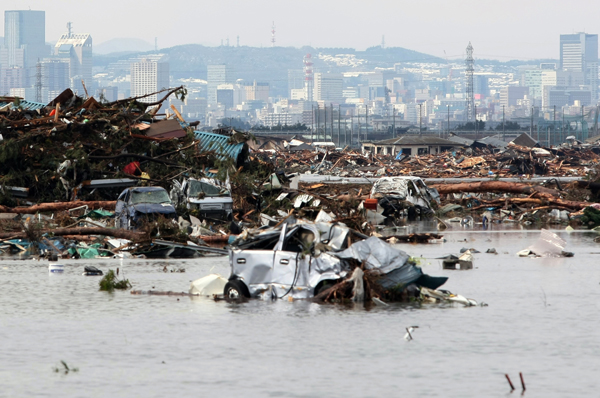
\includegraphics[width=\textwidth,height=0.8\textwidth]{Tsunami.jpg}
      \end{minipage}
      \hfill
      \begin{minipage}[t]{0.48\textwidth}
        \centering
        
        \caption*{Fukushima nuclear disaster. The nuclear reactor meltdown and hydrogen explosion.}
        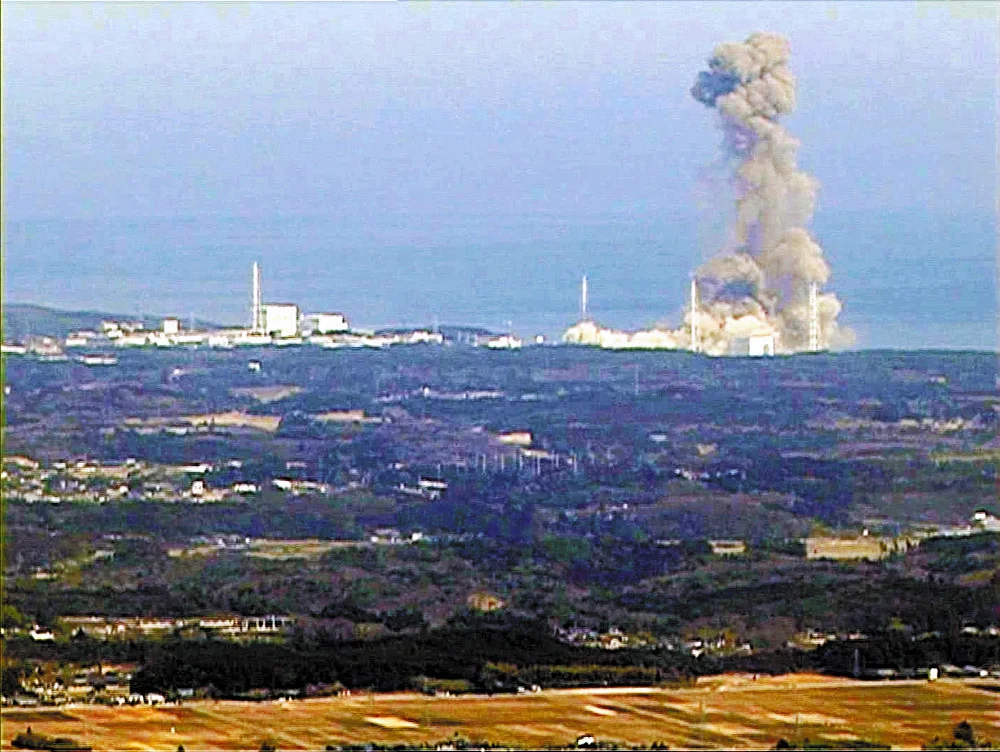
\includegraphics[width=\textwidth,height=0.8\textwidth]{Nuclear_explosion.png}
      \end{minipage}

    \end{figure}
    
    \end{minipage}
\end{frame}

%%%%%%%%%%%%%%%%%%%%%

\begin{frame}{Great East Japan Earthquake (March 2011)}


%Script draft%

% On the left map, the areas highlighted in green show the most affected prefectures. The total capital stock damages in the three hardest-hit prefectures, Iwate, Miyagi, and Fukushima, amount to 16 trillion yen. That's roughly 3.25% of Japan's GDP.

% The Fukushima nuclear disaster brought additional financial challenges, adding costs of 21.5 trillion yen for decommissioning, decontamination, and compensation.

% Additionally, the earthquake and tsunami led to massive evacuations, forcing up to 470,000 people to leave their homes across the country in just three days. At the peak, the percentage of evacuees reached 7.6% in Fukushima, 5.6% in Miyagi, and 3.4% in Iwate. This large-scale displacement disrupted daily life and the local economy, affecting employment and income stability for many families.

% Notably, in Fukushima, the number of evacuees outside the prefecture reached 59,464 at its peak, which is a significant difference compared to other affected prefectures.


    \begin{minipage}{1.00\textwidth}
    \raggedright
    \begin{flushleft}
\begin{table}[h!]
\vspace{-0.7cm}
\raggedright
Estimated total capital stock damages due to the earthquake and tsunami is 16 trillion Yen (3.25\% of GDP). Massive evacuations peaked at 470,000 people nationwide after 3 days.

\vspace{-0.04cm}
  \begin{minipage}[c]{0.4\textwidth}
    \includegraphics[width=\textwidth,height=1.10\textwidth]{epicenter.jpeg}
  \end{minipage}
\begin{minipage}[c]{0.51\textwidth}
    \raggedright
    \scalebox{0.75}{
    \begin{tabular}{|r|c|c|c|}
    \hline
    & \multicolumn{1}{c|}{Iwate} & \multicolumn{1}{c|}{Miyagi} & \multicolumn{1}{c|}{Fukushima} \\
    \hline
    Population (2010) & \multicolumn{1}{r|}{1,330,147} & \multicolumn{1}{r|}{2,348,165} & \multicolumn{1}{r|}{2,029,064} \\
    Deceased & \multicolumn{1}{r|}{4,675} & \multicolumn{1}{r|}{9,544} & \multicolumn{1}{r|}{1,614} \\
    Missing & \multicolumn{1}{r|}{1,110} & \multicolumn{1}{r|}{1,213} & \multicolumn{1}{r|}{196} \\
    Fully destroyed houses & \multicolumn{1}{r|}{20,185} & \multicolumn{1}{r|}{83,932} & \multicolumn{1}{r|}{20,136} \\
    Partially destroyed houses & \multicolumn{1}{r|}{4,562} & \multicolumn{1}{r|}{138,721} & \multicolumn{1}{r|}{65,093} \\
    In-pref. evacuees (Dec 2011) & \multicolumn{1}{r|}{43,953} & \multicolumn{1}{r|}{122,557} & \multicolumn{1}{r|}{95,200} \\
    Out-pref. evacuees (Dec 2011) & \multicolumn{1}{r|}{1,536} & \multicolumn{1}{r|}{8,603} & \multicolumn{1}{r|}{\textcolor{red}{59,464}} \\
    \hline
    \end{tabular}
    }
\end{minipage}


  \vspace{-1.6cm}
  \raggedleft{\small Table 1: Direct Damage Status of the Three Most Affected Prefectures}
\end{table}
\end{flushleft}
    \end{minipage}
    
\end{frame}
%%%%%%%%%%%%%%%%%%%%%%%%%%%%%%%%%%%%%

\begin{frame}[label=gender_income_gap]
\frametitle{Significant Wage Gap Between Regular and Non-Regular Employment in Japan (2022)}

%非正規雇用の問題は、日本の労働政策の主要な政策課題。失われた30年の期間、企業は正規雇用を非正規雇用に切り替えることでコストをさげ、延命してきた。女性で労働参加率は増加したが、日本の平均賃金は上がらず、デフレに苦しんできた。この傾向に、東日本大震災がどのような影響を与えたかが研究の関心事項の一つである。

%Script draft%

% Before talking about the gender income gap, let's examine the noticeable wage gap between regular and non-regular jobs in Japan as of 2022.

% The table shows that non-regular workers earn significantly less. This underscores the ongoing challenges in achieving fair wages in Japan, especially for gender income gap, since a higher percentage of non-regular workers are women compared to men.

% During the period known as the Lost 30 Years, many companies shifted from regular positions to non-regular ones to save money and stay open. This change led to an increase in non-regular jobs, particularly for women, and helped more people find work. However, even though more people are employed, average wages haven't increased, and Japan has been facing deflation. A key question I am exploring is how disasters have affected this trend.

The wage gap between regular and non-regular workers is a key concern in labor policy discussions.

\vspace{0.5cm}

\begin{table}[ht]
\centering
\begin{tabular}{l S[table-format=5.0] l}
\toprule
Employment Type & {Average Annual Income (\$)} & \\
\midrule
Regular Employment & 40846 & \\
Non-Regular Employment & 23538 & \textcolor{red}{(57.6\% of Regular)} \\
\bottomrule
\multicolumn{3}{r}{\footnotesize Note: Exchange rate \$1 = ¥130} \\
\end{tabular}
\caption{Average Annual Income by Employment Type}
\label{tab:average_income}
\end{table}

\gendergaplinks
\end{frame}

%%%%%%%%%%%%%%%%%%%%%%%%%%%%%%%%
\begin{frame}[label=employment_categories]
\frametitle{Employment Type Categories}

%Script draft%

% Here is the table of the employment types used in this study, and the definitions. These categories are based on the classifications from the Population Census. The first three categories—regular employees, executives, and self-employed—are considered regular workers. The last three categories—dispatched workers from temporary labor agencies, part-time or temporary employees and others, and family workers—are classified as non-regular workers.

% For each employment type, I conduct a Difference-in-Differences analysis using binary variables. This approach examines whether individuals are in each employment category or not, allowing us to assess the impact of disasters on different types of employment.


\textbf{Six employment type categories} in the Population Census.

\begin{table}[htbp]
\centering
\caption{Employment Types Categories in the Population Census}
\resizebox{0.75\textwidth}{!}{
\small
\begin{tabular}{>{\raggedright\arraybackslash}p{0.35\textwidth} >{\raggedright\arraybackslash}p{0.55\textwidth}}
\toprule
\textbf{Census Category} & \textbf{Definition} \\
\midrule
Regular employees & Regular employee has an indefinite employment contract with the employer. \\
\cmidrule{1-2}
Executives & Directors of a company or a corporation including managing directors. \\
\cmidrule{1-2}
Self-employed & Persons who ran a business with or without employees. \\
\midrule
Dispatched workers from temporary labour agency & Dispatched worker from temporary labour agency based on relevant laws. \\
\cmidrule{1-2}
Part-time/temporary employees and others & "Part-time worker", "Arbeit (temporary worker)" and "Contract employee or entrusted employee". \\
\cmidrule{1-2}
Family workers & Persons who worked in a business operated by a member of the household in which they lived. \\
\bottomrule
\end{tabular}
}
\label{tab:employment_status}

\end{table}

\vspace{-0.1cm}

\workersinks

\end{frame}

%%%%%%%%%%%%%%%%%%%%%%%%%%%%%%%%

%%%%%%%%%%%%%%%%%%%%%%%%%%%
%福島のEmployment type 割合
%%%%%%%%%%%%%%%%%%%%%%%%%%%

\begin{frame}[label=proportion_of_employment_type]
\frametitle{Proportion of Employment Types by Gender - Fukushima Pref. (2010)}

%Script draft%

% Now, let's look at the structure of the labor market by examining the types of employment among different genders in Fukushima Prefecture.

% Before the disaster, 62.7% of male workers were regular employees, while only 40.1% of female workers held regular positions. On the other hand, part-time jobs were much more common among women, with 37.9% working part-time compared to just 9.8% of men.

% This shows a significant difference in employment types between men and women. Understanding this labor market structure is crucial for assessing how the disaster affected the gender income gap. 

% Next, I will provide an overview of the wage gap between regular and non-regular employment in Japan.

\vspace{0.25cm} 
\returnbutton{different_types}{Return}

As the situation before the disaster, male workers had a higher proportion of \textbf{regular employees} (\textcolor{red}{62.7\%}) compared to female workers (\textcolor{red}{40.1\%}). Conversely, female workers had a significantly higher proportion of \textbf{part-time workers} (\textcolor{red}{37.9\%}) than male workers (\textcolor{red}{9.8\%}).

\vspace{1.0em} % Slight space added

\centering % Center the bar graph

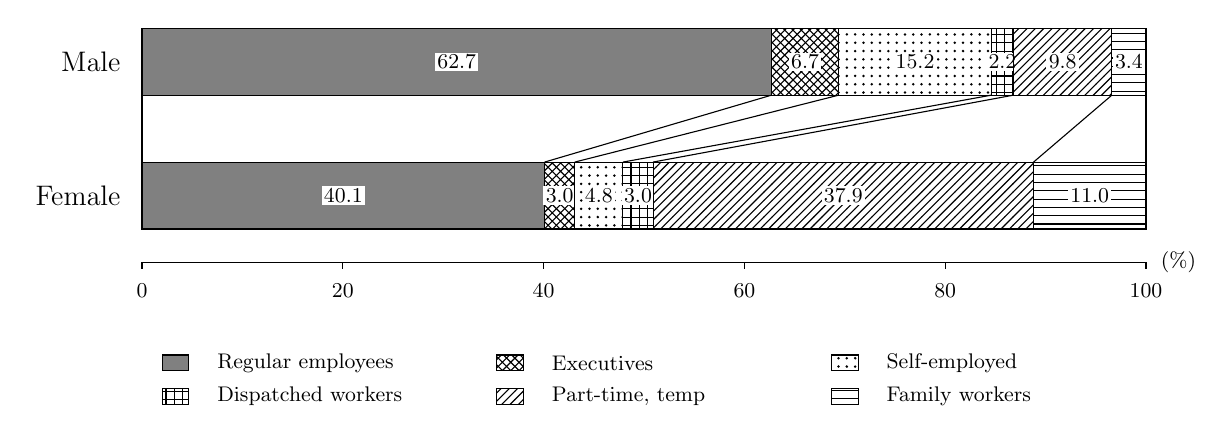
\begin{tikzpicture}[scale=0.85, transform shape]
    % Define colors
    \definecolor{color1}{RGB}{128,128,128}   % Regular employees
    \definecolor{color2}{RGB}{200,200,200}   % Executives
    \definecolor{color3}{RGB}{220,220,220}   % Self-employed
    \definecolor{color4}{RGB}{180,180,180}   % Dispatched workers
    \definecolor{color5}{RGB}{100,100,100}   % Part-time workers
    \definecolor{color6}{RGB}{60,60,60}      % Family workers

    % Bar length multiplier
    \def\barlength{15}

    % Male bar
    \draw[fill=color1] (0,10) rectangle (9.405,11) 
        node[pos=0.5, text=black, fill=white, inner sep=1pt] {\small 62.7};
    \draw[fill=color2, pattern=crosshatch] (9.405,10) rectangle (10.41,11) 
        node[pos=0.5, text=black, fill=white, inner sep=1pt] {\small 6.7};
    \draw[fill=color3, pattern=dots] (10.41,10) rectangle (12.69,11) 
        node[pos=0.5, text=black, fill=white, inner sep=1pt] {\small 15.2};
    \draw[fill=color4, pattern=grid] (12.69,10) rectangle (13.02,11) 
        node[pos=0.5, text=black, fill=white, inner sep=1pt] {\small 2.2};
    \draw[fill=color5, pattern=north east lines] (13.02,10) rectangle (14.49,11) 
        node[pos=0.5, text=black, fill=white, inner sep=1pt] {\small 9.8};
    \draw[fill=color6, pattern=horizontal lines] (14.49,10) rectangle (\barlength,11) 
        node[pos=0.5, text=black, fill=white, inner sep=1pt] {\small 3.4};

    % Female bar (updated)
    \draw[fill=color1] (0,8) rectangle (6.015,9) 
        node[pos=0.5, text=black, fill=white, inner sep=1pt] {\small 40.1};
    \draw[fill=color2, pattern=crosshatch] (6.015,8) rectangle (6.465,9) 
        node[pos=0.5, text=black, fill=white, inner sep=1pt] {\small 3.0};
    \draw[fill=color3, pattern=dots] (6.465,8) rectangle (7.185,9) 
        node[pos=0.5, text=black, fill=white, inner sep=1pt] {\small 4.8};
    \draw[fill=color4, pattern=grid] (7.185,8) rectangle (7.635,9) 
        node[pos=0.5, text=black, fill=white, inner sep=1pt] {\small 3.0};
    \draw[fill=color5, pattern=north east lines] (7.635,8) rectangle (13.32,9) 
        node[pos=0.5, text=black, fill=white, inner sep=1pt] {\small 37.9};
    \draw[fill=color6, pattern=horizontal lines] (13.32,8) rectangle (\barlength,9) 
        node[pos=0.5, text=black, fill=white, inner sep=1pt] {\small 11.0};

    % Auxiliary lines (updated for female bar)
    \draw[black, thin] (0,10) -- (0,9);
    \draw[black, thin] (9.405,10) -- (6.015,9);
    \draw[black, thin] (10.41,10) -- (6.465,9);
    \draw[black, thin] (12.69,10) -- (7.185,9);
    \draw[black, thin] (13.02,10) -- (7.635,9);
    \draw[black, thin] (14.49,10) -- (13.32,9);
    \draw[black, thin] (\barlength,10) -- (\barlength,9);

    % Labels
    \node[anchor=east] at (-0.2,10.5) {\large Male};
    \node[anchor=east] at (-0.2,8.5) {\large Female};

    % X-axis
    \draw (0,7.5) -- (\barlength,7.5);
    \foreach \x in {0,20,40,60,80,100} {
        \pgfmathsetmacro{\pos}{\x * \barlength / 100}
        \draw (\pos,7.5) -- (\pos,7.4) 
            node[anchor=north] at (\pos,7.3) {\small \x};
    }
    \node[anchor=west, font=\small] at (\barlength+0.1,7.5) {(\%)};

    % Adjusted Legend: shifted up and left by approximately 5 characters (~2.5cm)
    
    \begin{scope}[xshift=-2.0cm]
        % First Row
        \node[anchor=center, fill=color1, minimum width=0.4cm, minimum height=0.2cm, draw] at (2.5,6) {};
        \node[anchor=west] at (3,6) {\small Regular employees};
        
        \node[anchor=center, fill=color2, pattern=crosshatch, minimum width=0.4cm, minimum height=0.2cm, draw] at (7.5,6) {};
        \node[anchor=west] at (8,6) {\small Executives};
        
        \node[anchor=center, fill=color3, pattern=dots, minimum width=0.4cm, minimum height=0.2cm, draw] at (12.5,6) {};
        \node[anchor=west] at (13,6) {\small Self-employed};
        
        % Second Row
        \node[anchor=center, fill=color4, pattern=grid, minimum width=0.4cm, minimum height=0.2cm, draw] at (2.5,5.5) {};
        \node[anchor=west] at (3,5.5) {\small Dispatched workers};
        
        \node[anchor=center, fill=color5, pattern=north east lines, minimum width=0.4cm, minimum height=0.2cm, draw] at (7.5,5.5) {};
        \node[anchor=west] at (8,5.5) {\small Part-time, temp};
        
        \node[anchor=center, fill=color6, pattern=horizontal lines, minimum width=0.4cm, minimum height=0.2cm, draw] at (12.5,5.5) {};
        \node[anchor=west] at (13,5.5) {\small Family workers};
    \end{scope}
\end{tikzpicture}

\vspace{0em} % Space between the bar graph and legend

% \links placed inside the frame
\employmenttypelinks

\end{frame}

%%%%%%%%%%%%%%%%%%%%%%%%%%%%%%%%%%

%%%%%%%%%%%%%%%%%%%%%%%%%%%%%%%%
\section{Motivation \& Research Questions}
%%%%%%%%%%%%%%%%%%%%%%%%%%%%%%%%


\begin{frame}{Motivation \& Research Questions}
    \begin{center}
\vspace{-0.50cm} 

%Script draft%

% Here is the motivation behind my study and the research questions.

% Motivation:

% My study sits at the intersection of gender inequality and the impact of disasters. I aim to fill a research gap by examining how disasters affect gender disparities in the labor market. Additionally, the Fukushima experience provides valuable insights into the broader effects of nuclear accidents on employment and income in the area.

% Research Questions:

% The main question I’m looking at is whether the gender income gap gets bigger in areas hit by a disaster, focusing on the Great East Japan Earthquake. I chose this case because it was unique, involving a nuclear power plant accident that led to a large number of people evacuating. Also, I examine how this gap is affected by factors like the time period, gender, type of employment, and industry sector. The effects differ a lot depending on these various factors.

        \Large\textbf{Does the Gender Income Gap Expand in Areas Affected by a Disaster? Evidence from the Great East Japan Earthquake}
        \vspace{-0.3cm}
    \end{center}
    
    \vspace{0.7cm}
    
    \begin{columns}[T]
        \begin{column}{0.5\textwidth}
            \textbf{Motivation:}
            \begin{itemize}\small
                \item Gender inequality in disaster contexts
                \item Filling research gap on disaster-gender dynamics
                \item Informing policy for effective post-disaster recovery
            \end{itemize}
        \end{column}
        
        \begin{column}{0.5\textwidth}
            \textbf{Research Questions:}
            \begin{itemize}\small
                \item Does the gender income gap widen in the post-disaster period?
                \item How do impacts differ by:
                    \begin{itemize}\footnotesize
                        \item Time frame
                        \item Gender
                        \item Employment type
                        \item Industry sector
                    \end{itemize}
            \end{itemize}
        \end{column}
    \end{columns}
\end{frame}

%%%%%%%%%%%%%%%%%%%%%%%%%%%%%%%%
\section{Literature Review}
%%%%%%%%%%%%%%%%%%%%%%%%%%%%%%%%

\begin{frame}[label=literature_review1]
\frametitle{Literature review: Time Frames in the Economic Impact of Disasters}

%Script draft%

% A substantial body of research on the economic impacts of natural disasters employs difference-in-differences (DID) analysis and event study methodologies. Some empirical studies show the J-curve pattern observed in the economic impacts of natural disasters in developed countries. Studies using dynamic models and event study designs have found that areas affected by disasters typically go through three phases.

% In Phase 1, in the immediate aftermath, disasters lead to severe negative economic effects. Infrastructure is damaged, businesses are disrupted, and economic activity drops sharply.

% Phase 2 is the recovery phase. During this time, a reconstruction boom occurs as rebuilding efforts begin. This surge in construction helps recover the initial economic losses by creating jobs and attracting investments, especially in economically strong developed countries.

% In Phase 3, the economy returns to its normal trend. By this stage, the area has stabilized and is back to its pre-disaster economic path.

\vspace{-0.25cm}

Studies utilizing \textcolor{red}{DID analysis} and dynamic models, such as \textcolor{red}{event study designs}, have shown that disaster-affected areas in developed countries typically experience a \textcolor{red}{J-curve} pattern:


    \begin{minipage}[c]{0.4\linewidth}
        \small

        \vspace{-3.1cm}
        
\textcolor{red}{Short-term and long-term effects of natural disasters} (e.g., \citet{Deryugina2018TheReturns}, \citet{Canessa2021WomensShocks}, \citet{Kahraman2023AEarthquake}, \citet{Porcelli2019TheItaly}): 
\begin{itemize}
    \item Phase 1: Initial negative economic impact on disaster-affected areas.
    \item Phase 2: Recovery driven by reconstruction boom, offsetting initial negative impact((\ding{172}$<$\ding{173}) ).
    \item Phase 3: Return to pre-disaster trend (Returning to the steady state).
\end{itemize}

        \vspace{-3.0cm}
        

    \end{minipage}\hspace{0.1cm}
    \begin{minipage}{0.40\linewidth}
        \medskip
        \begin{figure}[h]
            \centering
            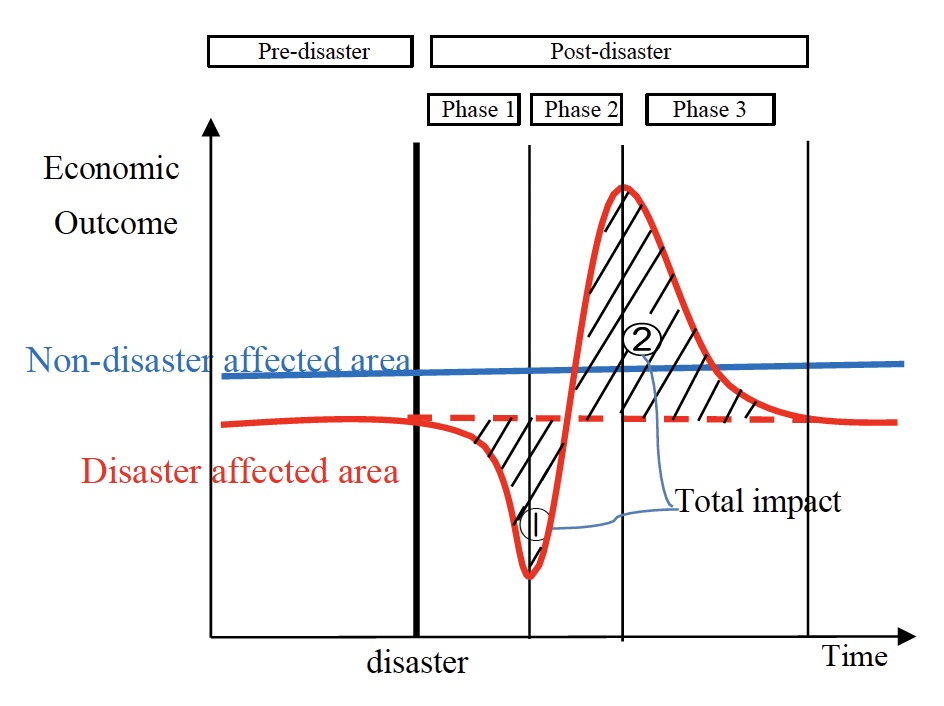
\includegraphics[height=.8\textheight]{conceptual_image.jpeg}
        \end{figure}
    \end{minipage}
    
\vspace{-0.4cm}

\eventstudyongrplinks

\end{frame}

%%%%%%%%%%%%%%%%%%%%%%%%%%%%%%%%%%%

\begin{frame}[label=literature_review2]
\frametitle{Literature Review: Theoretical Perspectives on Gender inequality in disaster contexts}


%Script draft%

% Here, I introduce two main theories: the Risk Adjustment Hypothesis and the Shock Coping Strategy Theory.

% First, the Risk Adjustment Hypothesis suggests that women are more vulnerable to labor market shocks during disasters. This means that during such events, women tend to face higher unemployment rates and experience significant income declines. This theory explains the decline in women's income.

% On the other hand, the Shock Coping Strategy Theory offers a different perspective. According to this theory, women may respond to disasters by increasing their participation in the labor market to cope with the adverse effects. This increased labor supply can lead to higher income and more employment opportunities for women. This theory explains the rise in women's income.

% These two theories provide contrasting insights into how disasters impact female income.

% The Great East Japan Earthquake showed that women were more suffered because they were overrepresented in non-regular jobs. Therefore, this study more focuses on the Phase 2 period.

The \textbf{Risk Adjustment Hypothesis} and the \textbf{Shock Coping Strategy} theory provide contrasting perspectives on the impact on the income of women in disaster-affected areas.

\vspace{0.2cm}

    \begin{table}[ht]
        \centering
        \begin{tabular}{>{\raggedright}p{3cm} p{10cm}}
            \hline
            \textbf{Theory} & \textbf{Key Insights} \\
            \hline

\addlinespace

            Risk Adjustment Hypothesis & Females are more vulnerable to labor market shocks during disasters, leading to higher unemployment rates and \textcolor{blue}{income declines}. (\citealt{Kim2014ARetention}; \citealt{Groger2016InternalTyphoon})\\

\addlinespace
            
            Shock Coping Strategy &  Females may increase their labor supply as a coping strategy to compensate for household income deficits, potentially \textcolor{red}{improving their income} and employment opportunities. (\citealt{Porcelli2019TheItaly}; \citealt{Deryugina2018TheReturns}; \citealt{Canessa2021WomensShocks})\\
            \hline
        \end{tabular}

        \label{tab:theoretical_perspectives}
    \end{table}
    
    \vspace{0.1cm}
    
\literaturelinks

\end{frame}
%%%%%%%%%%%%%%%%%%%%%%%%%%%%%%%%%%%


%%%%%%%%%%%%%%%%%%%%%%%%%%%%%%%%%%%
\section{Methodology}
%%%%%%%%%%%%%%%%%%%%%%%%%%%%%%%%%%%


%---------------------------------------
% Slide: Data
%---------------------------------------


%%%%%%%%%%%%%%%%%%%%%%%%%%%%%%%%
\begin{frame}[label=data]
\frametitle{Data Sets}

%Script draft%

% Here, this is a summary table for the data sets used in this study. I use two main sources of data: the JGSS and the national census.

% First, the JGSS is a social survey conducted by Osaka University. It targets residents living in Japan and is carried out every year or every other year. This survey covers a wide range of topics related to individual and family social attributes. The data is microdata at the individual level, providing detailed demographic information about each person.

% I also use data from the national census. The census surveys all residents of Japan and is conducted every five years. For our research, we utilize individual response data that has been made available specifically for academic studies. The sample size represents about 1% of the entire population, giving us a large and representative dataset to work with.

% In the analysis, I divide the survey years into two periods: before the disaster and after the disaster. In the table you see, the years before the disaster are shown in blue, and the years after the disaster are shown in red. I apply the same color-coding to both the census data and the JGSS data. This approach helps us clearly compare changes from before to after the disaster.

% Regarding the outcomes this study concerned with, for the JGSS, I examine the annual income bands of individuals, which indicate how much money people are earning each year. For the census data, I focus on employment status and employment type since the employment type is quite important factor for income level. This means I look at whether people are employed or unemployed, and what kinds of employment type they have.

% I limited the sample to include only the working population aged 15 and above. This ensures that focusing on those who are actively part of the labor market. I also exclude prefectures in major metropolitan areas because their economic conditions are very different from those in disaster-affected areas. By doing this, I reduce any bias that might come from including areas that are not directly comparable to the regions we are studying.

\begin{itemize}
    \item Two microdatasets randomly sampled from Japanese residents, reflecting population shares across prefectures.
    \item Descriptive statistics and Difference-in-Differences (DID) analysis with color-coded survey years (\textcolor{blue}{blue}: pre-disaster, \textcolor{red}{red}: post-disaster), focusing on long run effects of the disaster.
\end{itemize}

\vspace{-0.1cm}
\begin{figure}
    \centering
    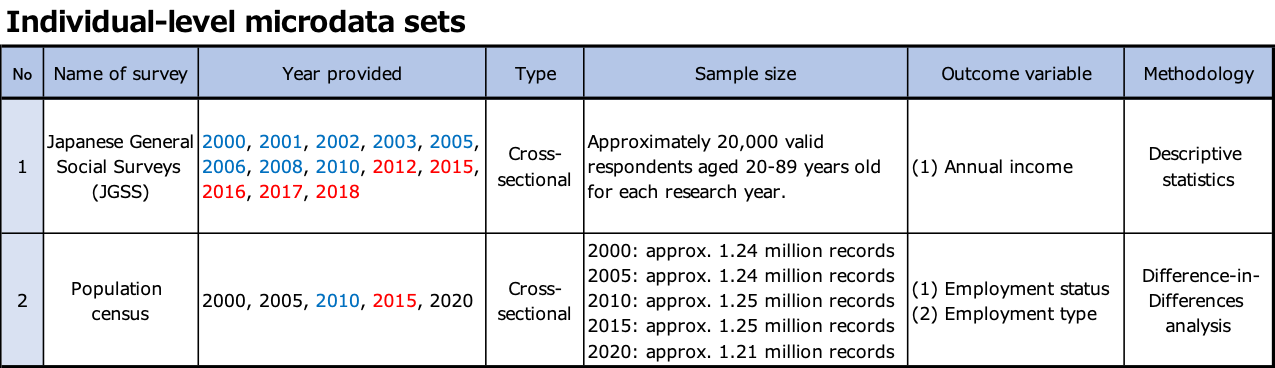
\includegraphics[width=0.93\textwidth]{datasets.png}
\end{figure}

\datalinks

\end{frame}
%%%%%%%%%%%%%%%%%%%%%%%%%%%%%%%%

%%%%%%%%%%%%%%%%%%%%%%%%%%%%%%%%

\begin{frame}[label=treatment_control_groups]
\frametitle{Treatment and Control Groups in Datasets}

%Script draft%

% Here are the treatment and control groups for two datasets. Each analysis is conducted separately for males and females.

% In the JGSS Analysis, the treatment group includes Iwate, Miyagi, and Fukushima prefectures, while the control group consists of all other prefectures.

% For the Census DID Analysis, Fukushima is the treatment group, and the control group includes other prefectures excluding major cities like Tokyo and Osaka.


Treatment and Control groups used in two datasets: JGSS and Population Census.

\begin{table}[htbp]
\centering
\caption{JGSS Descriptive Statistics Analysis (analyzed by gender)}
\resizebox{0.9\textwidth}{!}{
\small
\begin{tabular}{>{\raggedright\arraybackslash}p{0.2\textwidth} >{\raggedright\arraybackslash}p{0.65\textwidth}}
\toprule
\textbf{Group} & \textbf{Prefectures} \\
\midrule
Treatment & Three Most Affected Prefectures (Iwate, Miyagi, Fukushima) \\
\cmidrule{1-2}
Control & Other prefectures \\
\bottomrule
\end{tabular}
}

\end{table}


\begin{table}[htbp]
\centering
\caption{Population Census DID Analysis (estimated by gender)}
\resizebox{0.9\textwidth}{!}{
\small
\begin{tabular}{>{\raggedright\arraybackslash}p{0.2\textwidth} >{\raggedright\arraybackslash}p{0.65\textwidth}}
\toprule
\textbf{Group} & \textbf{Prefectures} \\
\midrule
Treatment & Fukushima \\
\cmidrule{1-2}
Control & Other prefectures excluding metropolitan areas (Tokyo, Kanagawa, Saitama, Chiba, Osaka, Kyoto, Hyogo, Nara, Aichi, Gifu, Mie) \\
\bottomrule
\end{tabular}
}

\end{table}

\end{frame}

%%%%%%%%%%%%%%%%%%%%%%%%%%%%%%%%%%%%%%


\begin{frame}{Methodology and Empirical Strategy: Descriptive Statistics and  Difference-in-Differences}

%Script draft%

% Moving on to the methodology and empirical strategy, this study uses a basic Difference-in-Differences analysis with individual-level data from the Population Census. For the JGSS data, I perform a descriptive analysis on average income.

% The DID estimator, beta 2, is a central focus of this research. I estimate the Difference-in-Differences model separately for male and female groups. This approach compares changes in outcome variables before and after the disaster between Fukushima Prefecture and other prefectures for each gender. The gap between the DID coefficients for males and females is a key aspect of the study, highlighting the different impacts that disasters may have based on gender.

% In the model, I include control variables related to household composition and living arrangements to ensure the results are accurate. These controls account for factors like age group, marital status, how long individuals have lived in their current residence, their relationship to the household head, the type of residence, and household size. The model also includes prefecture fixed effects, and the error term is clustered at the prefecture level.

\vspace{-0.2cm}
A \textcolor{red}{Difference-in-Differences (DID) analysis} on Population Census data, restricting the sample to the population aged 15 and over, and excluding metropolitan areas. The sample is divided into male and female and estimated the disaster's impact on outcome variables of concern.
\vspace{-0.1cm}
   \begin{equation}
   \Large Y_{ipt} = \alpha + \beta_1 \text{Post}_t + \beta_2 (\text{Fukushima}_p \cdot \text{Post}_t) + \gamma X_{ipt} + \delta_p + \epsilon_{ipt}
   \end{equation}
   \vspace{-0.5cm}
   \begin{itemize}
   \item $Y_{ipt}$ denotes the outcome variable for employment status or employment type for individual $i$ in prefecture $p$ at year $t$.
   \item $\text{Fukushima}_p$ is a binary indicator for Fukushima Prefecture.
   \item $\text{Post}_t$ is a binary indicator for the post-disaster year (2015), with the pre-disaster year (2010).
   \item \textcolor{red}{$\beta_2$ represents the DID estimate, capturing the disaster's impact} on the probability of being the employment status or type.
   \item $X_{ipt}$ are individual control variables including age group, marital status, residence duration, relationship with household head, residence type, and household size.
   \item $\delta_p$ represents prefecture fixed effects.
   \end{itemize}
\end{frame}

%%%%%%%%%%%%%%%%%%%%%%%%%%%%%%%%
\section{Results}
%%%%%%%%%%%%%%%%%%%%%%%%%%%%%%%%

\begin{frame}[label=income_band_main]
\frametitle{Income Bands by Gender: Pre- (2000-2010) vs Post-Disaster (2012-2018) - JGSS}

%Script draft%

% Here are the results from the descriptive analysis of the JGSS. The sample is divided by gender and prefecture, as shown in the table, and average income is compared. The table shows how the average income levels changed from before the disaster to after the disaster.

% The analysis highlights that women in the three affected prefectures saw a notable increase in their income levels. Specifically, women in these areas had a 9.79% rise in mean annual income after the disaster, and this increase is statistically significant.

% Looking at the kernel density graph, the blue line represents the distribution of income bands during the pre-disaster period, while the red line shows the distribution in the post-disaster period. The income distribution shifts to the right only for women in the affected areas, as shown in the bottom left graph. This means that after the disaster, women in these prefectures experienced higher income levels.

    \vspace{-0.7cm}
    \begin{columns}[T, onlytextwidth]
        % テーブルを左側に配置
        \begin{column}{0.5\textwidth}
            \begin{table}[ht]
                \scriptsize
                \setlength{\tabcolsep}{4pt}
                \renewcommand{\arraystretch}{1.0}
                \begin{tabular}{lccccc}
                    \toprule
                    \multirow{2}{*}{Gender} & \multirow{2}{*}{Prefecture} & \multicolumn{2}{c}{Mean Income} & \multirow{2}{*}{Change (\%)} & \multirow{2}{*}{P-value} \\
                    & & Pre & Post & & \\
                    \midrule
                    \multirow{2}{*}{Male} 
                        & Affected & \textcolor{blue}{7.967} & \textcolor{red}{7.835} & -1.67 & 0.654 \\
                        & Unaffected & \textcolor{blue}{8.660} & \textcolor{red}{8.300} & \quad -4.16*** & 0.000 \\
                    \midrule
                    \multirow{2}{*}{Female} 
                        & Affected & \textcolor{blue}{4.721} & \textcolor{red}{5.183} & +9.79* & 0.065 \\
                        & Unaffected & \textcolor{blue}{4.995} & \textcolor{red}{5.087} & +1.83 & 0.143 \\
                    \bottomrule
                    \multicolumn{6}{@{}p{\textwidth}}{\footnotesize $*p<0.1$, $**p<0.05$, $***p<0.01$} \\
                \end{tabular}
                \caption{Mean Annual Income from Main Job: Pre/Post-Disaster Period (Income bands, N=20,119)}
                \label{tab:income}
            \end{table}
        \end{column}
        
        % 図を右側に配置
        \begin{column}{0.485\textwidth}
            \begin{figure}[ht]
                \centering
                \includegraphics[width=\textwidth]{Kernel density graphs of respondent’s annual income from main job.png}
                \caption{Kernel Density of Annual Income from Main Job (Income bands, N=20,119)}
                \label{fig:kde_income}
            \end{figure}
        \end{column}
    \end{columns}
    
    % 説明文をスライドの下部に配置
    \begin{column}{0.49\textwidth}
            \raggedright
    
    \vspace{-2.5cm}
    \hspace{-1.1cm}
\large {\qquad \ \ \ \ Females in the three affected prefectures experienced the largest income increase (+9.79\%) post-disaster (a rightward shift (increase) in average income bands when comparing pre- and post-disaster periods).}
    \end{column}
\vspace{-0.7cm}
\incomebandlinks
\end{frame}
%%%%%%%%%%%%%%%%%%%%%%%%%%%%%%%%%%%

\begin{frame}[label=employed]


%Script draft%

% The next analysis uses a difference-in-differences approach with individual-level census data, comparing Fukushima to other prefectures outside of major metropolitan areas. I looked at males and females separately. The outcome variable is whether someone is employed or not. The table shows different models based on the control variables I included, with Models 3 and 6 being the most comprehensive. The results reveal that the disaster had a bigger positive impact on male employment, increasing it by 2.1 to 2.6 percentage points, compared to a smaller increase of 0.5 percentage points for female employment, as shown by the DID estimator in the top row of the table.

\textbf{Employment Status:} The disaster had a larger positive impact on male employment (2.1-2.6 percentage points) compared to females (0.5 percentage points).

\begin{table}[htbp]
\centering
\caption{DID Estimates of Disaster Impact on Employment Status}

\vspace{-0.2cm}

\scalefont{0.57}

\begin{tabular}{@{}l*{6}{c}@{}}
          &\multicolumn{3}{c}{Male}                                &\multicolumn{3}{c}{Female}                              \\\cmidrule(lr){2-4}\cmidrule(lr){5-7}
          &\multicolumn{1}{c}{(1)}         &\multicolumn{1}{c}{(2)}         &\multicolumn{1}{c}{(3)}         &\multicolumn{1}{c}{(4)}         &\multicolumn{1}{c}{(5)}         &\multicolumn{1}{c}{(6)}         \\
\toprule
Disaster Impact (DID)&    \textcolor{red}{0.023\sym{***}}&    \textcolor{red}{0.021\sym{***}}&    \textcolor{red}{0.026\sym{***}}&    \textcolor{red}{0.005\sym{***}}&   \textcolor{red}{-0.000}         &    \textcolor{red}{0.005\sym{***}}\\
          &  (0.002)         &  (0.002)         &  (0.002)         &  (0.001)         &  (0.001)         &  (0.001)         \\
\addlinespace
Post-Disaster Period&   -0.006\sym{***}&    0.017\sym{***}&    0.022\sym{***}&    0.011\sym{***}&    0.029\sym{***}&    0.033\sym{***}\\
          &  (0.002)         &  (0.002)         &  (0.002)         &  (0.001)         &  (0.001)         &  (0.001)         \\
\addlinespace
Married   &                  &    0.191\sym{***}&    0.117\sym{***}&                  &   -0.062\sym{***}&   -0.046\sym{***}\\
          &                  &  (0.005)         &  (0.002)         &                  &  (0.005)         &  (0.005)         \\
\midrule
Age Group   &       No         &      Yes         &      Yes         &       No         &      Yes         &      Yes         \\
Residence Duration&       No         &       No         &      Yes         &       No         &       No         &      Yes         \\
Relationship with Head&       No         &       No         &      Yes         &       No         &       No         &      Yes         \\
Residence Type&       No         &       No         &      Yes         &       No         &       No         &      Yes         \\
Household Size&       No         &       No         &      Yes         &       No         &       No         &      Yes         \\
$\textit{N}$&  540,474         &  540,474         &  540,474         &  598,422         &  598,422         &  598,422         \\
$\textit{R}^2$&    0.003         &    0.385         &    0.430         &    0.003         &    0.295         &    0.318         \\
Control Mean&    0.644         &    0.644         &    0.644         &    0.455         &    0.455         &    0.455         \\
\bottomrule
\end{tabular}
\\\\{\linewidth}{\tiny Standard errors clustered at prefecture level in parentheses}\\\\
\\\\{\linewidth}{\tiny $*p<0.1$, $**p<0.05$, $***p<0.01$}\\\\
\\\\{\linewidth}{\tiny \textit{Note}: This table presents OLS estimates of the impact of the disaster on employment status for both males and females (aged 15 years and over) under different model specifications, excluding metropolitan areas. The outcome variable is a binary indicator where individuals are categorized as employed if they were working, and as not employed if they were seeking work (completely unemployed), engaged in housework, attending school, or in other situations. All models include prefecture fixed effects, and the error term is clustered at the prefecture level. Control Mean represents the average employment rate in non-Fukushima prefectures before the disaster period.}
\end{table}

\vspace{-2.2cm}
\employmentprobabilitylinks


\end{frame}

%%%%%%%%%%%%%%%%%%%%%%%%%%%%%%%%

%%%%%%%%%%%%%%%%%%%%%%%%%%%%%%%%
%\cmidrule(lr){2-2}\cmidrule(lr){3-3}\cmidrule(lr){4-4}\cmidrule(lr){5-5}\cmidrule(lr){6-6}\cmidrule(lr){7-7}
%%%%%%%%%%%%%%%%%%%%%%%%%%%%%%%%%%%

\begin{frame}[label=different_types]

%Script draft%

% Next, I analyze the data using the same difference-in-differences approach, looking at different types of employment. The outcome variable is the probability of being employed in each employment type. I used 2010 and 2015 survey years for the main DID, and I also conducted placebo test using 2000 and 2005 survey years to check pre-trend.

% The result of main DID is, for men, the probability of becoming a regular employee increased by 2.4 percentage points after the disaster. However, for women, there was little to no change in regular employment. On the other hand, women saw a decrease in other job categories. Specifically, there were negative impacts on dispatched workers, part-time workers, and family workers.

% These results highlight that the disaster had a positive effect on men's regular employment but had minimal or even negative effects on women's employment in non-regular positions.


\textbf{Each Employment Type:} For males, the probability of becoming a regular employee increased by 2.4 percentage points, while the effect for females was insignificant. In contrast, females experienced negative impacts in dispatched worker, part-time worker, and family worker.

\vspace{-0.20cm}

\begin{table}[htbp]
\centering
\caption{DID Estimates of Disaster Impact on Different Employment Types by Gender}

\vspace{-0.5cm}

\resizebox{\linewidth}{!}{%
\begin{tabular}{@{}l*{17}{c}@{}}
          &\multicolumn{2}{c}{Regular Employee} &\multicolumn{2}{c}{Executive}        &\multicolumn{2}{c}{Self-employed}    &\multicolumn{2}{c}{Dispatched Worker}&\multicolumn{2}{c}{Part-time Worker} &\multicolumn{2}{c}{Family Worker}    &\multicolumn{2}{c}{Unknown Worker}   \\\cmidrule(lr){2-3}\cmidrule(lr){4-5}\cmidrule(lr){6-7}\cmidrule(lr){8-9}\cmidrule(lr){10-11}\cmidrule(lr){12-13}\cmidrule(lr){14-15}
          &\multicolumn{1}{c}{(1)}&\multicolumn{1}{c}{(2)}&\multicolumn{1}{c}{(3)}&\multicolumn{1}{c}{(4)}&\multicolumn{1}{c}{(5)}&\multicolumn{1}{c}{(6)}&\multicolumn{1}{c}{(7)}&\multicolumn{1}{c}{(8)}&\multicolumn{1}{c}{(9)}&\multicolumn{1}{c}{(10)}&\multicolumn{1}{c}{(11)}&\multicolumn{1}{c}{(12)}&\multicolumn{1}{c}{(13)}&\multicolumn{1}{c}{(14)}\\
          &\multicolumn{1}{c}{Male}&\multicolumn{1}{c}{Female}&\multicolumn{1}{c}{Male}&\multicolumn{1}{c}{Female}&\multicolumn{1}{c}{Male}&\multicolumn{1}{c}{Female}&\multicolumn{1}{c}{Male}&\multicolumn{1}{c}{Female}&\multicolumn{1}{c}{Male}&\multicolumn{1}{c}{Female}&\multicolumn{1}{c}{Male}&\multicolumn{1}{c}{Female}&\multicolumn{1}{c}{Male}&\multicolumn{1}{c}{Female}\\
\toprule
Disaster Impact (DID)&    \textcolor{red}{0.024\sym{***}}&    \textcolor{red}{0.001}         &   \textcolor{red}{-0.000}         &    \textcolor{red}{0.003\sym{***}}&   \textcolor{red}{-0.007\sym{***}}&    \textcolor{red}{0.001\sym{*}}  &   \textcolor{red}{-0.001}         &   \textcolor{red}{-0.003\sym{***}}&    \textcolor{red}{0.001}         &   \textcolor{red}{-0.001}         &   \textcolor{red}{-0.002\sym{***}}&   \textcolor{red}{-0.001\sym{*}}  &    \textcolor{red}{0.011\sym{***}}&    \textcolor{red}{0.005\sym{***}}\\
          &  (0.001)         &  (0.001)         &  (0.001)         &  (0.000)         &  (0.001)         &  (0.000)         &  (0.000)         &  (0.000)         &  (0.001)         &  (0.001)         &  (0.000)         &  (0.001)         &  (0.001)         &  (0.001)         \\
\addlinespace
Post-Disaster Period&    0.029\sym{***}&    0.018\sym{***}&   -0.003\sym{***}&   -0.000         &   -0.008\sym{***}&   -0.000         &    0.001\sym{***}&    0.001\sym{***}&    0.004\sym{***}&    0.019\sym{***}&   -0.001\sym{***}&   -0.004\sym{***}&   -0.001         &   -0.000         \\
          &  (0.001)         &  (0.001)         &  (0.001)         &  (0.000)         &  (0.001)         &  (0.000)         &  (0.000)         &  (0.000)         &  (0.001)         &  (0.001)         &  (0.000)         &  (0.000)         &  (0.001)         &  (0.001)         \\
\addlinespace
Married   &    0.123\sym{***}&   -0.042\sym{***}&    0.025\sym{***}&   -0.002\sym{***}&   -0.000         &   -0.015\sym{***}&   -0.009\sym{***}&   -0.006\sym{***}&   -0.029\sym{***}&    0.004         &    0.004\sym{***}&    0.018\sym{***}&    0.003\sym{***}&   -0.003\sym{**} \\
          &  (0.003)         &  (0.005)         &  (0.001)         &  (0.001)         &  (0.002)         &  (0.001)         &  (0.001)         &  (0.001)         &  (0.002)         &  (0.003)         &  (0.001)         &  (0.001)         &  (0.001)         &  (0.001)         \\
\addlinespace
Age Group &      Yes         &      Yes         &      Yes         &      Yes         &      Yes         &      Yes         &      Yes         &      Yes         &      Yes         &      Yes         &      Yes         &      Yes         &      Yes         &      Yes         \\
\addlinespace
Residence Duration &      Yes         &      Yes         &      Yes         &      Yes         &      Yes         &      Yes         &      Yes         &      Yes         &      Yes         &      Yes         &      Yes         &      Yes         &      Yes         &      Yes         \\
\addlinespace
Relationship with Head &      Yes         &      Yes         &      Yes         &      Yes         &      Yes         &      Yes         &      Yes         &      Yes         &      Yes         &      Yes         &      Yes         &      Yes         &      Yes         &      Yes         \\
\addlinespace
Residence Type &      Yes         &      Yes         &      Yes         &      Yes         &      Yes         &      Yes         &      Yes         &      Yes         &      Yes         &      Yes         &      Yes         &      Yes         &      Yes         &      Yes         \\
\addlinespace
Household Size &      Yes         &      Yes         &      Yes         &      Yes         &      Yes         &      Yes         &      Yes         &      Yes         &      Yes         &      Yes         &      Yes         &      Yes         &      Yes         &      Yes         \\
\midrule
$\textit{N}$&  540,474         &  598,422         &  540,474         &  598,422         &  540,474         &  598,422         &  540,474         &  598,422         &  540,474         &  598,422         &  540,474         &  598,422         &  540,474         &  598,422         \\
$\textit{R}^2$&    0.389         &    0.183         &    0.026         &    0.008         &    0.060         &    0.014         &    0.010         &    0.016         &    0.046         &    0.112         &    0.022         &    0.039         &    0.108         &    0.060         \\
Control Mean&    0.400         &    0.173         &    0.043         &    0.013         &    0.093         &    0.024         &    0.011         &    0.012         &    0.071         &    0.185         &    0.011         &    0.039         &    0.015         &    0.009         \\
\bottomrule
\end{tabular}}
\raggedright
\\\\{\linewidth}{\tiny Standard errors clustered at prefecture level in parentheses}\\\\
\vspace{-0.2cm}
\\\\{\linewidth}{\tiny $*p<0.1$, $**p<0.05$, $***p<0.01$}\\\\
\\\\{\linewidth}{\tiny \textit{Note}: This table presents DID estimates of the impact of the disaster on different employment types by gender. The dependent variable for each model is a binary indicator for the respective employment type. All models include prefecture fixed effects, age group, residence duration, relationship with head, residence type, and household size fixed effects. The error term is clustered at the prefecture level. The binary variable for marital status assigns 1 to those with a spouse present and 0 to those never married, widowed, or divorced. Metropolitan areas (Tokyo, Kanagawa, Saitama, Chiba, Osaka, Kyoto, Hyogo, and Aichi) are excluded from the analysis. Control Mean represents the mean of the dependent variable for the control group (non-Fukushima) in the pre-disaster period.}
\end{table}

\vspace{-3.2cm}
\differentemploymenttypeslinks

\end{frame}

%%%%%%%%%%%%%%%%%%%%%%%%%%%%%%%%%%%

\begin{frame}[label=summary]
\frametitle{Key Findings}

%Script draft%

% In my previous JGSS analysis, I discovered that women’s average income in disaster-affected areas increased significantly compared to men's income. Nevertheless, the DID analysis on population census indicates that women experienced limited gains in regular employment, whereas men saw substantial improvements in securing regular jobs. Notably, women had fewer opportunities for non-regular employment, including dispatched, part-time, and family roles. Given these contrasting outcomes in employment and earnings, the next section explores how the evacuation of primarily working population from Fukushima Prefecture and changes in the industry structure have impacted the labor market and women's average income in the prefecture.

{\Large
\begin{itemize}
    \item First, women’s average income in Fukushima showed significant increases compared to other groups.
    
    \item Nevertheless, DID analysis shows that women saw limited gains in regular employment, while men experienced significant improvements in regular employment. Notably, women had decreased proportions for non-regular employment types.
    
    \item[$\Rightarrow$] \textcolor{blue}{Given the contrasting results in employment and earnings, the following analysis examines structural change of industry and outmigration's impact.}
\end{itemize}
}
\end{frame}

%%%%%%%%%%%%%%%%%%%%%%%%%

\begin{frame}[label=numbers_of_workers]
\frametitle{Difference in the Number of Workers in Fukushima (2010 vs 2015)}

\vspace{-0.2cm}

%Script draft%

% To understand the gender differences in out-migration, let's see the table highlights significant gender differences in employment changes from 2010 to 2015 in Fukushima Prefecture. Male employment increased slightly by 1,289 workers, primarily driven by a substantial rise in the construction industry, which added 13,740 male workers. In contrast, female employment decreased markedly by 14,626 workers, with no similar growth in the construction sector for women.

% The decline in female employment was especially pronounced in non-regular positions, which saw a decrease of 13,108 workers. This significant reduction in female non-regular employment may explain the substantial increase in average income for women after the disaster, as fewer women remained in lower-paying, non-regular jobs. The decline suggests that many female workers in these roles did not return to Fukushima during the evacuees' return phase. 

% Consequently, this apperes as the observed gender gap in net outmigration, with more men choosing to return compared to women.

% With low-wage workers leaving the labor market, the average wage of the remaining workers increases. This is because those who stay typically have higher wages, which raises the overall average. It's important to note that there might be a potential upward bias in these findings due to selection bias.

The significant decrease in female non-regular employment may explain the substantial increase in average income for women post-disaster. \textcolor{red}{Potential upward bias due to selection bias}.

\vspace{-0.2cm}

\begin{table}[htbp]
\centering
\caption{Difference in the Number of Workers (2010 vs 2015) in Fukushima}

\vspace{-0.2cm}

\scalefont{0.60}

\begin{tabular}{
    l
    S[table-format=6.0]           % Male Total
    S[table-format=6.0]           % Male Regular
    S[table-format=6.0]           % Male Non-regular
    S[table-format=7.0]           % Female Total
    S[table-format=6.0]           % Female Regular
    S[table-format=6.0]           % Female Non-regular
}
\toprule
\multirow{2}{*}{Occupation} & \multicolumn{3}{c}{Male} & \multicolumn{3}{c}{Female} \\
\cmidrule(lr){2-4} \cmidrule(lr){5-7}
& {Total} & {Regular} & {Non-regular} 
& {Total} & {Regular} & {Non-regular} \\
\midrule
\textbf{Total} & \textbf{\quad 1289} & \textbf{\quad \ -545} & \textbf{\quad 1834} & \textbf{\ \ -14626} & \textbf{\quad -1518} & \textbf{-13108} \\
Admin.\& managerial & -84 & -28 & -52 & 141 & 173 & -14 \\
Prof.\& technical & 3521 & 3186 & 335 & 2629 & 1957 & 672 \\
Clerical & 9364 & 7612 & 1752 & 4734 & 2516 & 2218 \\
Sales & -9636 & -8513 & -1123 & -6188 & -2072 & -4116 \\
Service & -1069 & -441 & -628 & -2922 & 284 & -3206 \\
Security & 1184 & 1094 & 90 & -33 & 87 & -120 \\
Agri., forest.\& fish. & -6669 & -5959 & -710 & -3950 & -127 & -3823 \\
\textcolor{red}{Constr.\& mining} & \textcolor{red}{\ \ 13740} & \textcolor{red}{\ \ 11435} & \textcolor{red}{\quad \ 2319} & \textcolor{red}{\qquad \ \ 328} & \textcolor{red}{\qquad \ 96} & \textcolor{red}{\qquad 222} \\
Manufacturing & -14864 & -12017 & -2847 & -8632 & -4003 & -4629 \\
Trans.\& machine op. & 1042 & 596 & 446 & 103 & 78 & 25 \\
Carrying,\ clean.,\ pack. & 7279 & 4519 & 2760 & 646 & 12 & 634 \\
Not Classifiable & -2569 & -2049 & -520 & -1502 & -519 & -983 \\
\bottomrule
\end{tabular}

\addlinespace[0.35em]

\raggedright
\scriptsize
\textit{Note}: Positive values indicate an increase in the number of workers, while negative values indicate a decrease.

\end{table}

\vspace{-0.2cm}
\numbersofworkerslinks

\end{frame}


%%%%%%%%%%%%%%%%%%%%%%%%%%%%%%%%
\section{Conclusion}
%%%%%%%%%%%%%%%%%%%%%%%%%%%%%%%%

\begin{frame}[label=summary]
\frametitle{Conclusion}

%Script draft%

% In conclusion, the Fukushima disaster initially affected women more severely because they were primarily employed in non-regular jobs. During the recovery phase, the evacuation led to a gender-based selection bias. Combined with how families adapted, this caused women's average incomes to rise faster than men's, even though men secured more regular jobs.

% However, this apparent increase in women’s incomes from snapshot data can be misleading for policymakers. To gain a clearer understanding, an event study using panel data is necessary to properly account for selection bias.


{\Large
\begin{itemize}

\item The evacuation may have led to a \textcolor{red}{gender-differentiated selection bias} which, combined with \textcolor{red}{shock coping strategies}, resulted in women's average income increasing faster than men's during Phase 2, despite men achieving more substantial gains in regular employment.

\item The apparent increase in women's average income observed in cross-sectional data may lead to misleading policy implications.

  \vspace{0.3cm}
  \hspace{1cm} $\Rightarrow$ \textcolor{blue}{A panel dataset event study analysis would be an appropriate approach to control for selection bias.}
\end{itemize}
}
\end{frame}

%%%%%%%%%%%%%%%%%%%%%%%%%%%%%%%%
\begin{frame}[label=conclusion]

\frametitle{For Further Research: A Framework for the Dynamics of the Gender Income Gap}


%Script draft%

% In conclusion, the study identified three key phases in how the gender income gap changed after the disaster.

% First, Phase 1 showed that women were more affected because many worked in non-regular employment type. This supports the Risk Adjustment Hypothesis.

% Next, Phase 2 revealed that women's incomes increased. This happened because of househpld coping strategies and the evacuation changed which women remained in the area. This created an upward bias in their incomes.

% Finally, Phase 3 indicates a return to a steady state, where the income gap begins to stabilize over time.

% Although it might seem extra, a possible framework for future research is proposed as shown in the figure on the right. This framework focuses on removing selection bias and using a dynamics model to analyze the disaster's impact over time.

% The study found that the disaster's impacts are heterogeneous across periods, gender, occupation, and industry, and can help shape policies to address these inequalities. 

% Thank you for your attention. I’d be happy to answer any questions or hear your suggestions.


    \begin{minipage}[c]{0.4\linewidth}
        \small

        \vspace{-1.4cm}
        

{\footnotesize


\begin{itemize} 

\item Phase 1: Women are disproportionately affected due to their overrepresentation in non-regular employment (\textcolor{red}{Risk Adjustment Hypothesis}). 
\item Phase 2: Women's incomes rose due to \textcolor{red}{coping strategies} and \textcolor{red}{selection bias} (Evacuation changed the composition of female worker's employment type remaining in the area, introducing an upward bias in income). 
\item Phase 3: Returning to the steady state. 
\end{itemize}

}

{\tiny
Magnitude of Impact on the Gender Income Gap:
}


{\tiny
\begin{equation}
\int_{T0}^{T2} [YF_F(t) - YF_C(t)] dt
\end{equation}
}

{\tiny
where $YF_F(t)$ represents the female worker's income in disaster affected area at time $t$, and $YF_C(t)$ represents the counterfactual which assumes the earthquake did not occur.
}

        
        \vspace{-2.1cm}

    \end{minipage}\hspace{0.5cm}
    \begin{minipage}{0.2\linewidth}
        \medskip
        \begin{figure}[h]
            \centering
            \fbox{
    \mbox{
        \small Possible Analytical Framework for Further Research
    }
}
    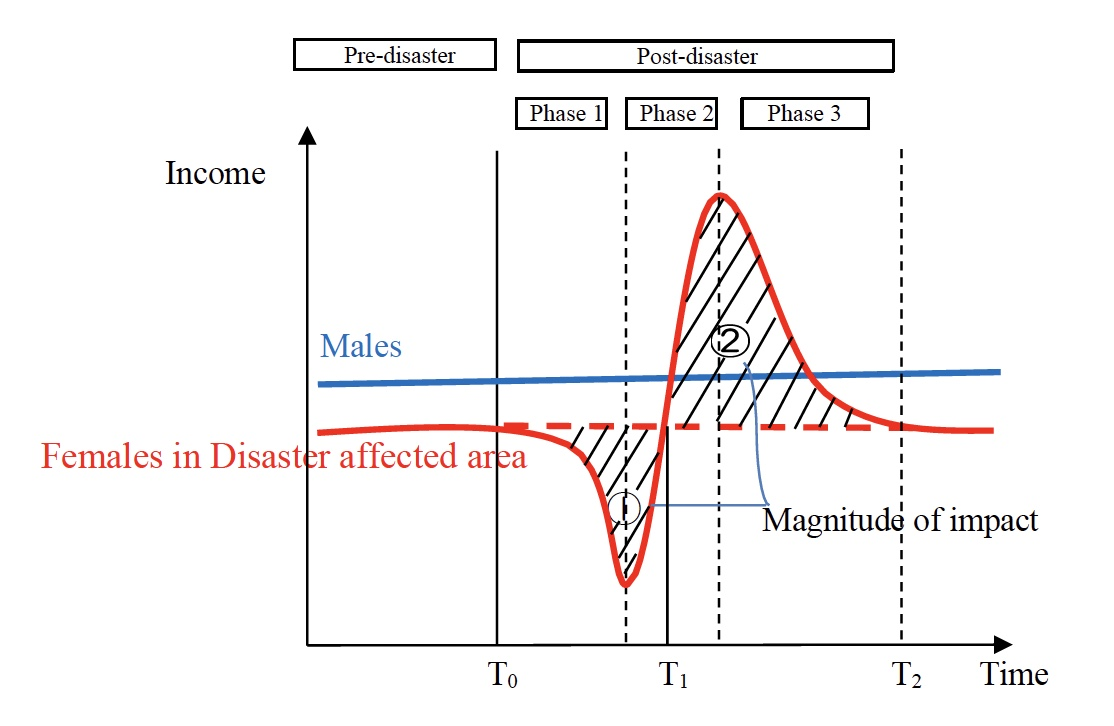
\includegraphics[height=.7\textheight]{Final_conceptual_model.jpeg}
        \end{figure}
    \end{minipage}

\conclusionlinks


\end{frame}

%%%%%%%%%%%%%%%%%%%%%%%%%%%%

%%%%%%%%%%%%%%%%%%%%%%%%%%%%%%%%
%---------------------------------------
\begin{frame}
    \begin{center}
        {\Huge\calligra Thank You}
    \end{center}
\end{frame}
%---------------------------------------
%%%%%%%%%%%%%%%%%%%%%%%%%%%%%%%%


% アペンディックスセクションの開始
\appendix  % この行が重要です!

%%%%%%%%%%%%%%%%%%%%%%%%%%%%%%%%
\section{Appendix}
%%%%%%%%%%%%%%%%%%%%%%%%%%%%%%%%
\begin{frame}
    \centering
    \Huge \textbf{Appendix}
\end{frame}
%%%%%%%%%%%%%%%%%%%%%%%%%%%%%%%%%%%

\begin{frame}[label=evacuees_main]
\frametitle{Total Number of Internal and External Evacuees by Prefecture (2011-2021)}

%Script draft%

% The table here presents the total number of internal and external evacuees by prefecture from 2011 to 2021, focusing on Iwate, Miyagi, and Fukushima.

% On the right, there’s a graph illustrating the trend of evacuees over these years. Notice that Fukushima experienced a longer period of displacement compared to Miyagi and Iwate.

% While all three prefectures have seen a decrease in evacuees over the past decade, Fukushima faces unique challenges. The extended displacement has impacted the local workforce, particularly because many young people left Fukushima due to safety concerns related to nuclear contamination.

\vspace{-0.38cm} 
\returnbutton{outmigration}{Return}

    \vspace{0.3cm}
    \begin{columns}[T, onlytextwidth]
        % Table on the left
        \begin{column}{0.5\textwidth}
            \begin{table}[ht]
                \scriptsize
                \setlength{\tabcolsep}{4pt}
                \renewcommand{\arraystretch}{1.0}
                \begin{tabular}{@{}lS[table-format=6.0]S[table-format=6.0]S[table-format=6.0]S[table-format=6.0]S[table-format=6.0]@{}}
                \toprule
                Prefecture & {2011} & {2013} & {2015} & {2017} & {2021} \\
                \midrule
                Iwate & 45489 & 37426 & 25021 & 10440 & 1557 \\
                Miyagi & 131160 & 99449 & 56739 & 15530 & 4682 \\
                Fukushima & 154664 & 136656 & 101272 & 52287 & 34074 \\
                \midrule
                Total & 331313 & 273531 & 183032 & 78257 & 40313 \\
                \bottomrule
                \end{tabular}
                \caption{Total Number of Evacuees by Prefecture}
                \label{tab:evacuees}
            \end{table}
        \end{column}
        
        % Figure on the right (placeholder)
        \begin{column}{0.485\textwidth}
            \begin{figure}[ht]
                \centering
                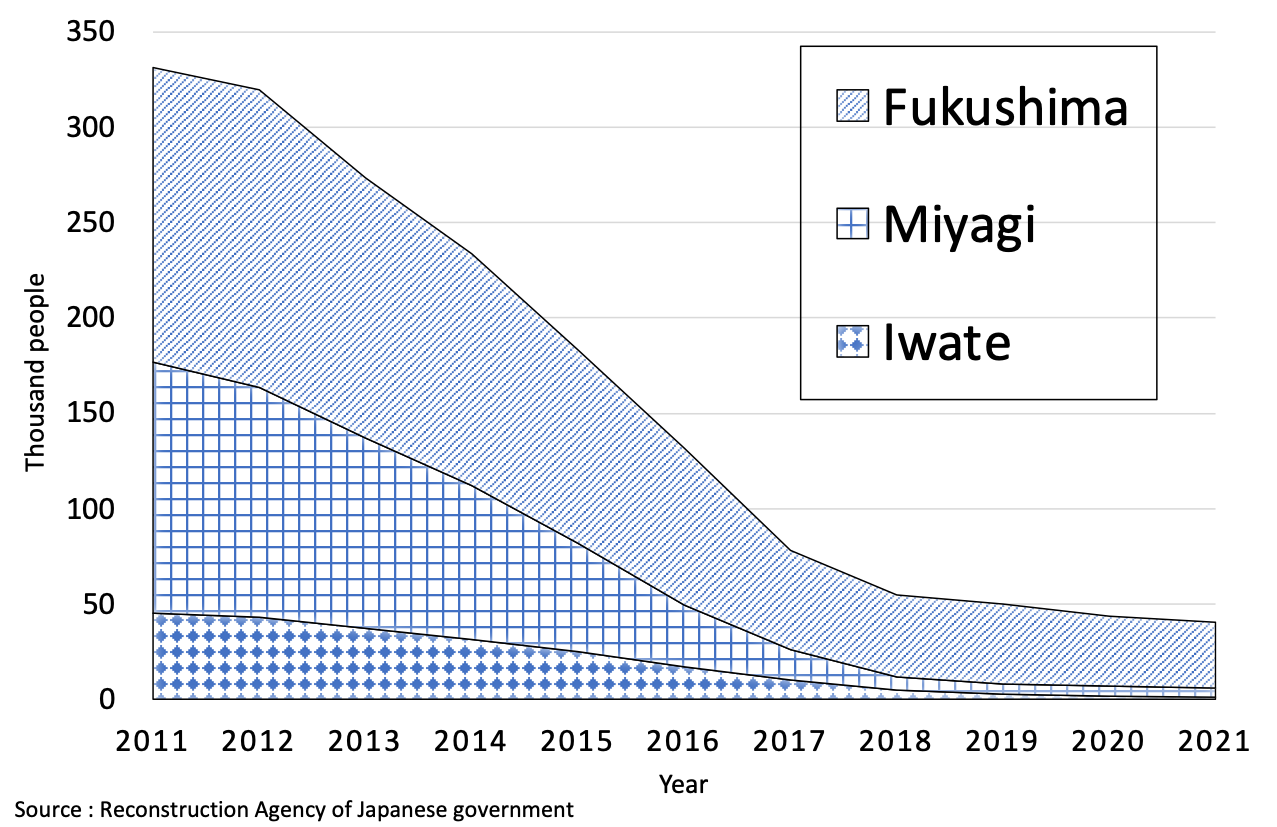
\includegraphics[width=\textwidth]{evacuation2.png}
                \caption{Trend of Evacuees by Prefecture}
                \label{fig:evacuees_trend}
            \end{figure}
        \end{column}
    \end{columns}
    
% Explanation text at the bottom of the slide
\begin{column}{0.49\textwidth}
    \raggedright
    \vspace{-2.5cm}
    \hspace{-1.1cm}
    \small{
        \begin{itemize}
            \item Longer displacement in Fukushima
            \item Prolonged evacuation and youth outflow
            \item Significant impact on local labor markets

        \end{itemize}
    }
\end{column}
\vspace{-0.5cm}
\end{frame}

%%%%%%%%%%%%%%%%%%%%%%%%%%%%%
%%%%%%%%%%%%%%%%%%%%%%%%%%%%%%%%%%%

\begin{frame}[label=short_term_unemployment]
\frametitle{Short-term changes
in unemployment insurance recipients in Fukushima}


\vspace{0.25cm} 
\returnbutton{event_study_results}{Return}

The ratio of women unemployment insurance recipients in Fukushima increased sharply after the disaster, surpassing the national average.

    \vspace{0.2cm}

    \centering
    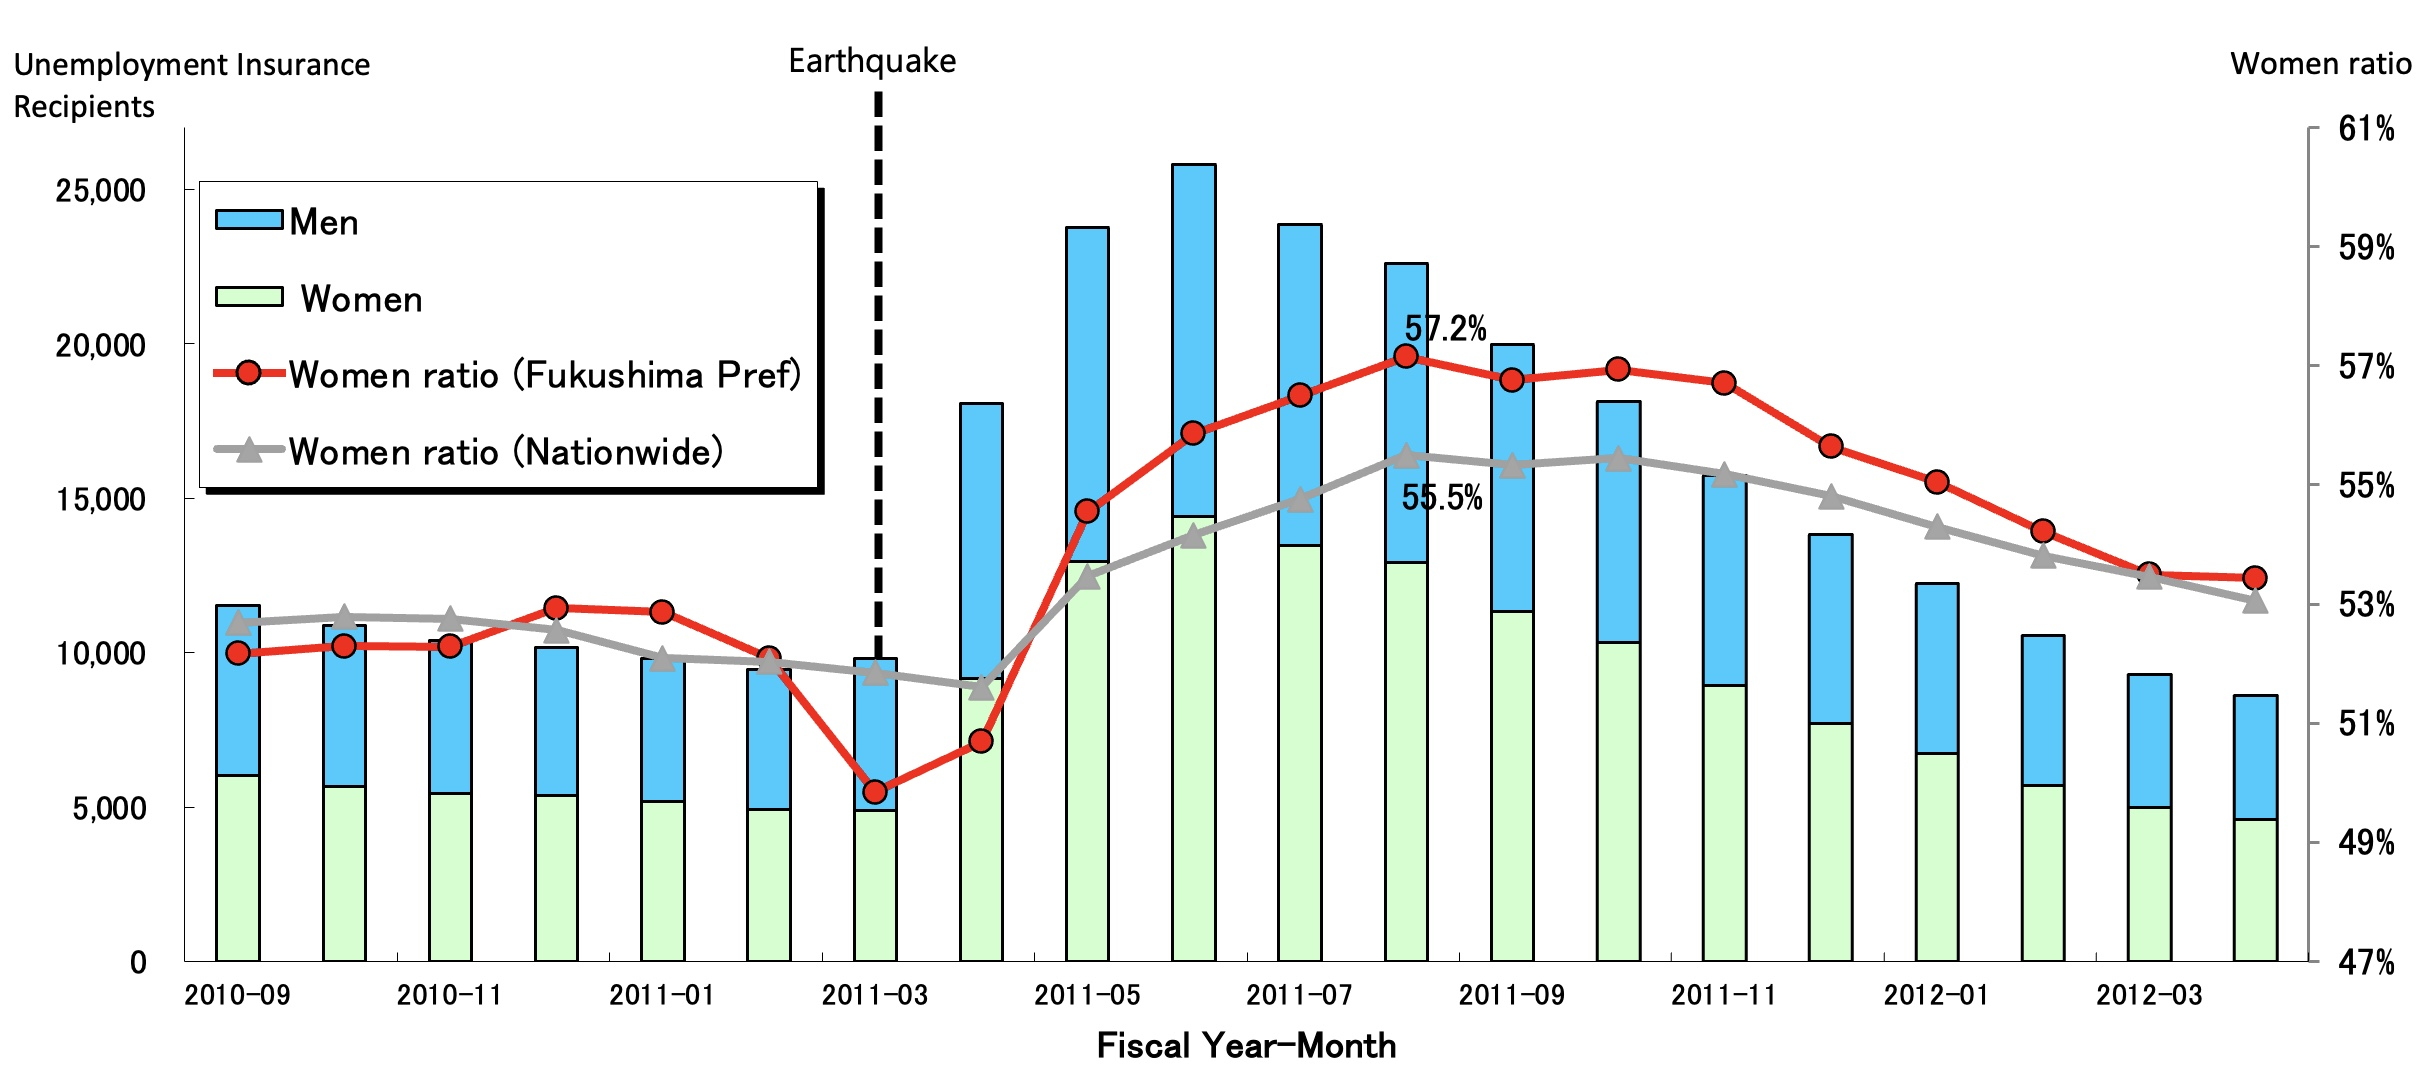
\includegraphics[width=0.8\textwidth]{Number of Actual unemployment insurance recipants (short-term).jpeg}
    \vspace{0.5cm}

\begin{minipage}{0.8\textwidth}
    {\small
        {}
    }
\end{minipage}

\unemploymentinsurancelinks

\end{frame}
%%%%%%%%%%%%%%%%%%%%%%%%%%%%%%%%


\begin{frame}[label=unemploymentinsurance]
\frametitle{Short-term (upper graph) and long-term (lower graph) changes
in unemployment insurance recipients in Fukushima}

\vspace{0.25cm} 
\returnbutton{event_study_results}{Return}


    \begin{minipage}[c]{0.4\linewidth}
        \small


        \vspace{-2.3cm}
        
        Reversal of Short-term and Long-term Trends:
        \begin{itemize}
            \item The ratio of women unemployment insurance recipients in Fukushima increased sharply after the disaster, surpassing the national average.

            \item However, in the longer term, the women's ratio in Fukushima fell below the national average, indicating a reversal of the initial trend.

        \end{itemize}
        
        \vspace{-2.1cm}
        

    \end{minipage}\hspace{0.5cm}
    \begin{minipage}{0.40\linewidth}
        \medskip
        \begin{figure}[h]
            \centering
            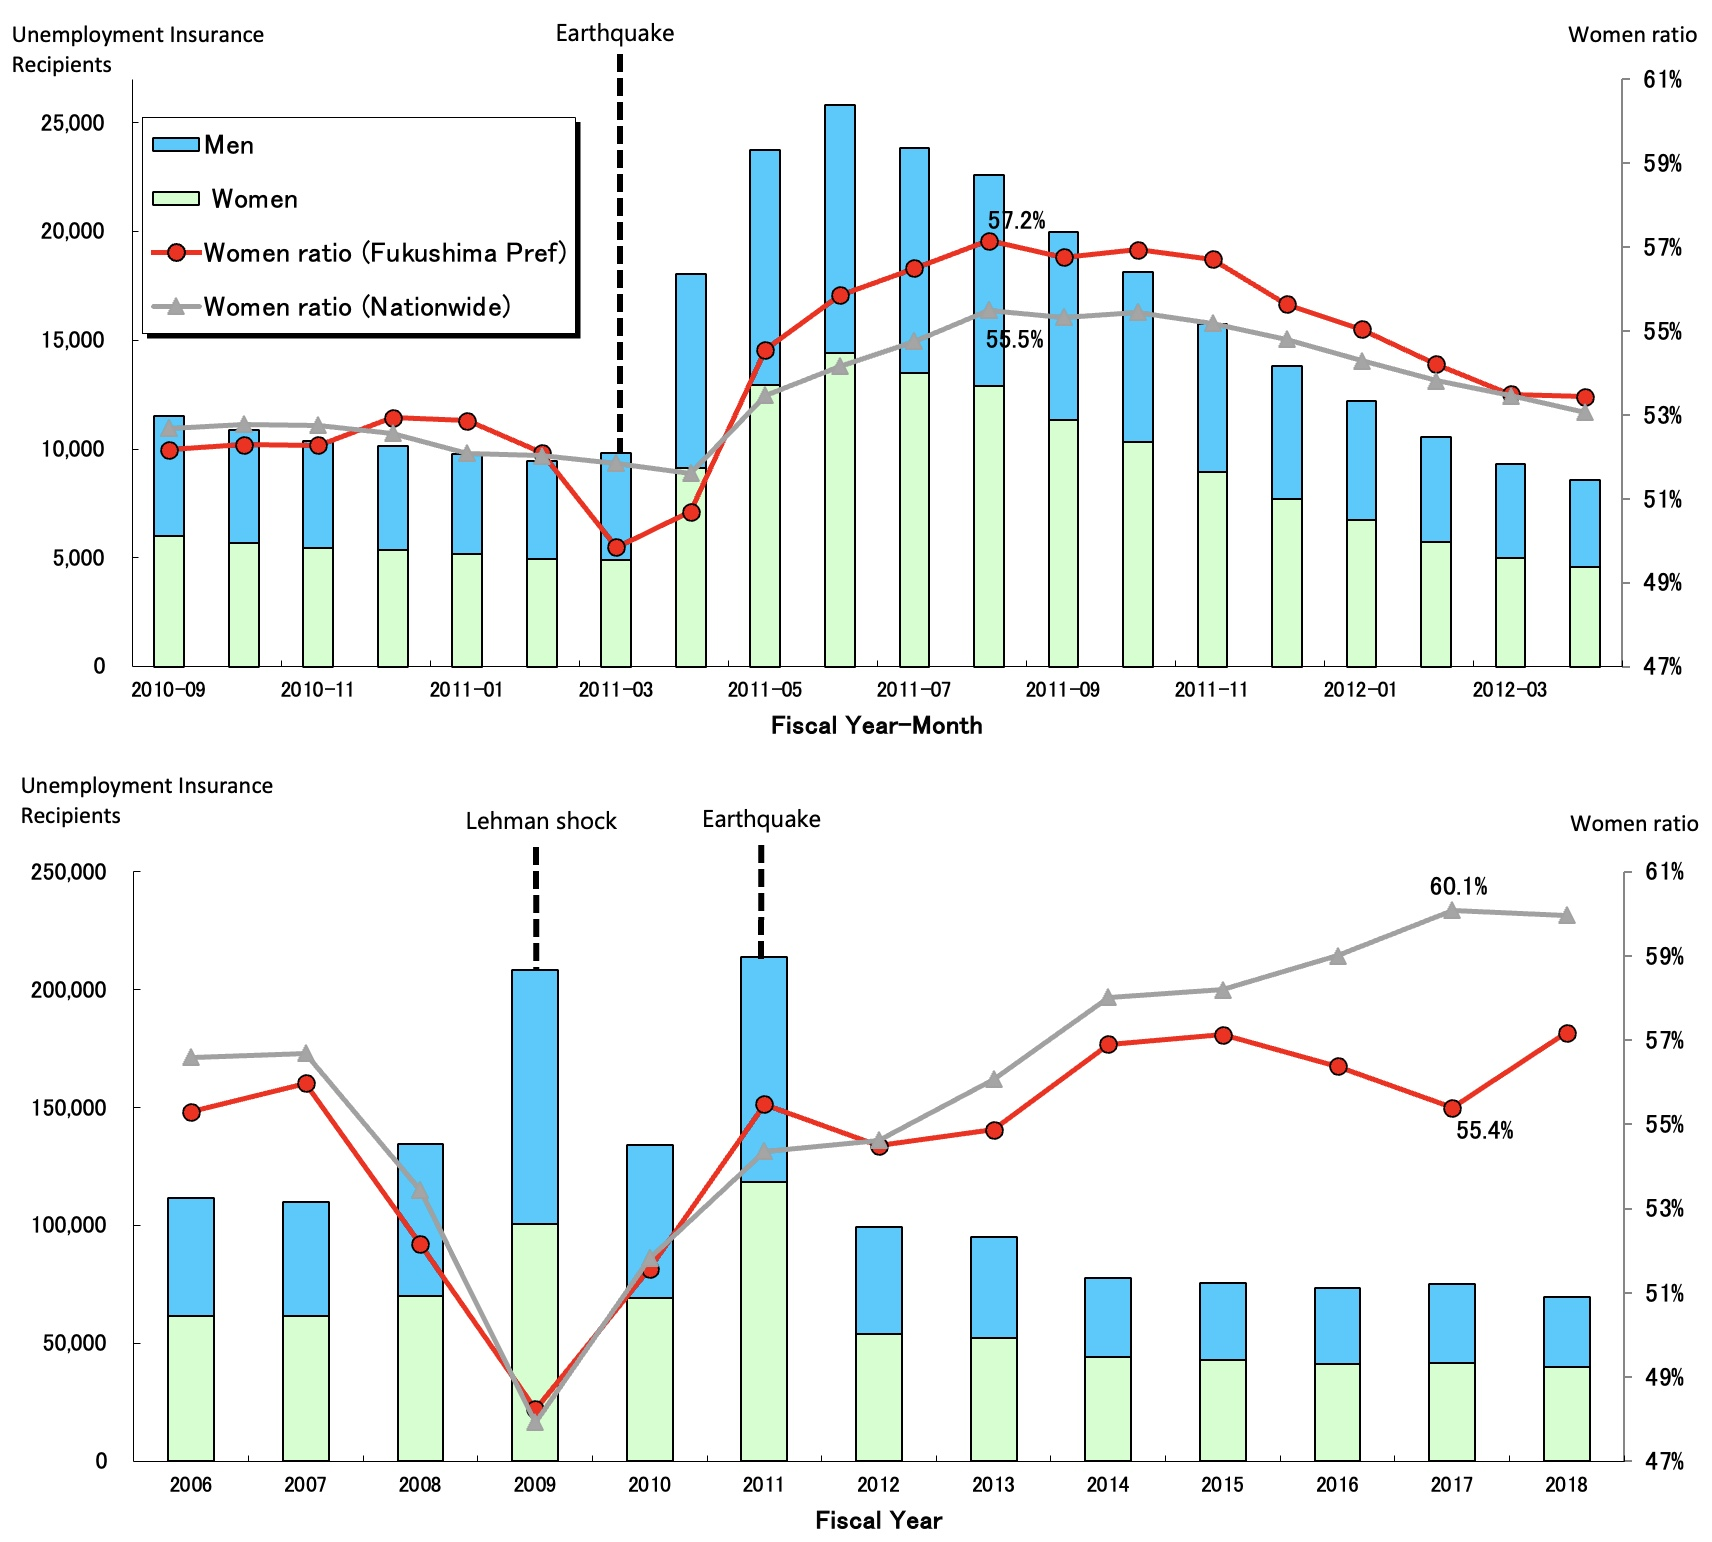
\includegraphics[height=.81\textheight]{Number of Actual Unemployment Insurance Recipients3.jpeg}
        \end{figure}
    \end{minipage}
\end{frame}
%%%%%%%%%%%%%%%%%%%%%%%%%%%%%%%%%%%
%%%%%%%%%%%%%%%%%%%%%%%%%%%%%%%%%
\begin{frame}[label=event_study_results]
\frametitle{Event Study Analysis: Impact of 2011 Great East Japan Earthquake}

\vspace{0.20cm}

\returnbutton{conclusion}{Return}

\vspace{-0.20cm}

The event study analysis of the disaster's impact on \textcolor{red}{regional production} aligns with previous literature, showing initial negative effects followed by recovery and long-term positive outcomes.

    \begin{minipage}[c]{0.4\linewidth}
        \small
        \vspace{-1.6cm}
        
Event Study on Gross Regional Production (GRP) in the Affected Prefectures:

\vspace{-0.3cm}

\fontsize{8}{10}\selectfont
\begin{equation}
\ln(GRP_{it}) = \alpha_i + \lambda_t + \sum_{k=2006}^{2017} \beta_k \cdot Treat_i \cdot 1[t-2010=k] + \epsilon_{it}
\end{equation}

\normalsize

\begin{itemize}
    \item Phase 1: Immediate severe negative impact (-9.3\% in 2011).
    \item Phase 2: Recovery and positive trend from 2013, peaking at +2.6\% in 2014.
    \item Phase 3: Sustained positive effects through 2017, gradually normalizing.
\end{itemize}
        
        \vspace{-2.0cm}
        
\end{minipage}\hspace{0.56cm}
    \begin{minipage}{0.3\linewidth}
        \medskip
        \begin{figure}[h]
            \centering
            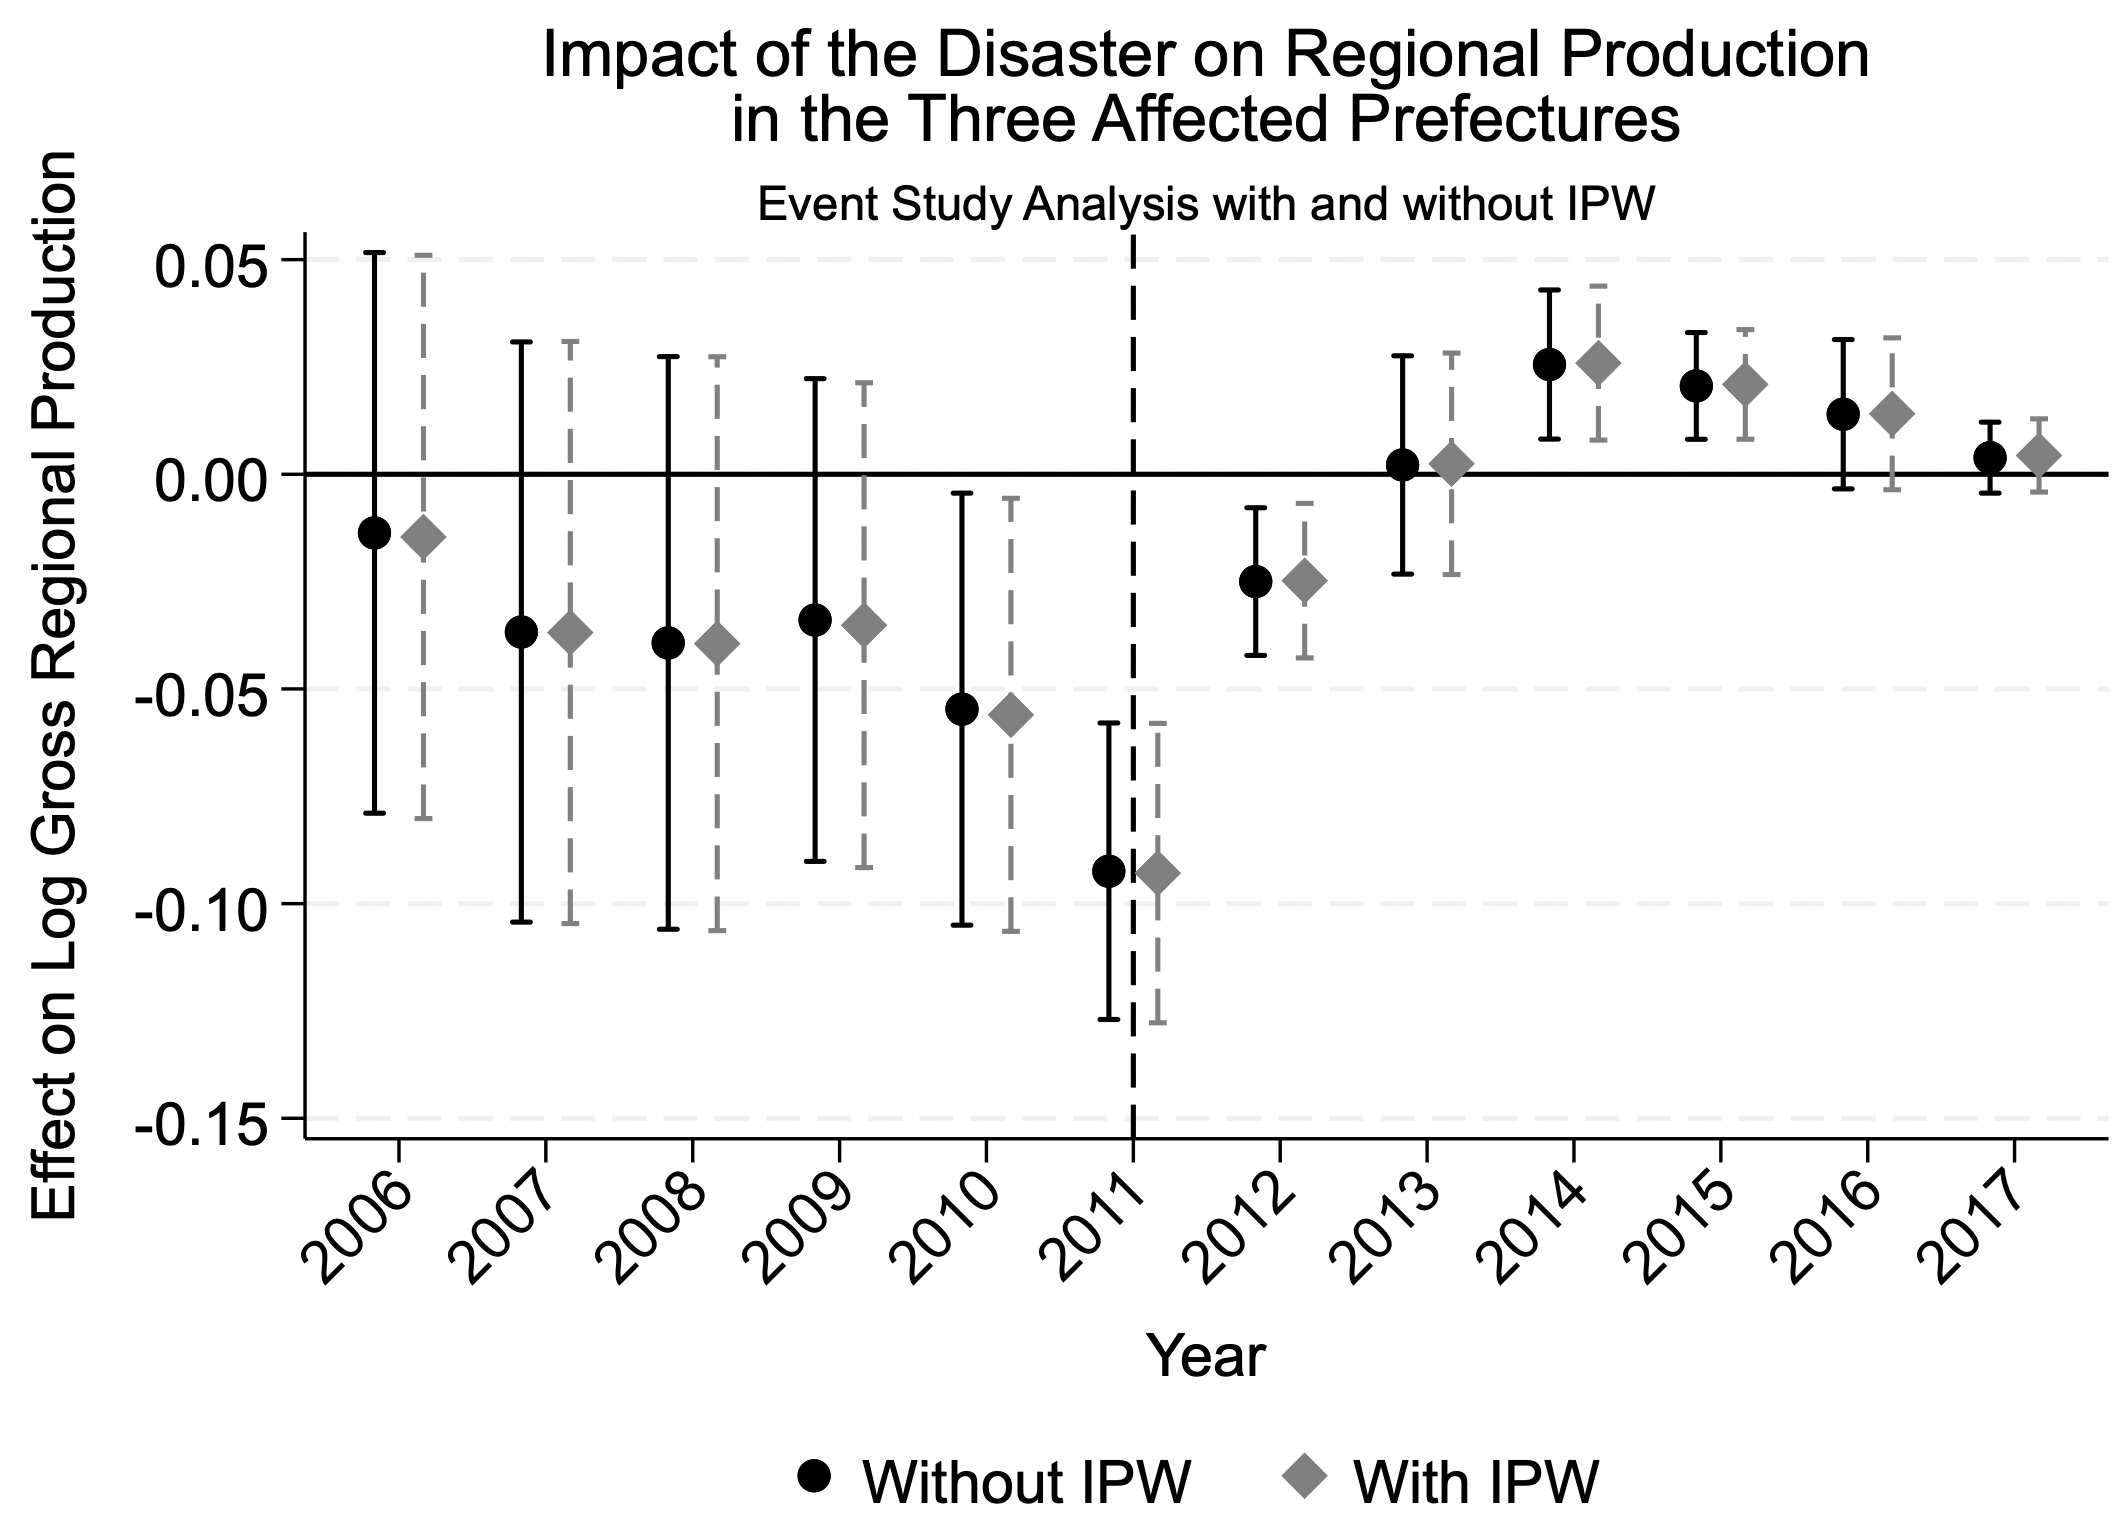
\includegraphics[height=.75\textheight]{event_study_results.jpeg}
        \end{figure}
    \end{minipage}

    \vspace{-0.15cm}
\longtermimpactlinks
\end{frame}

%---------------------------------------
% Slide: Literature Review - Risk Adjustment Hypothesis
%---------------------------------------

\begin{frame}[label=risk_adjustment_hypothesis]
\frametitle{Literature Review: Risk Adjustment Hypothesis}

\vspace{-1.0cm} 
\returnbutton{literature_review2}{Return}


    Nearly every empirical study of natural disasters finds short-term declines in either income or employment, especially for groups vulnerable to disasters, such as primary industry workers, non-regular workers, women, and the elderly.
    
    \vspace{0.3cm}
    
    \textbf{Key Studies:}
    \begin{itemize}
        \item \citet{Kim2014ARetention}: Analyzed the 2010 Haiti earthquake, revealing employment rates dropped from 52.6\% to 28.6\% five months post-disaster. Notably, only 34.2\% of women retained employment compared to 55.6\% of men.
        \item \citet{Groger2016InternalTyphoon}: Studied Typhoon Ketsana in Vietnam, finding affected households experienced a 10\% income decline due to crop losses. Internal labor migration to urban areas was a key coping mechanism.
    \end{itemize}
    
\end{frame}

%---------------------------------------
% Slide: Literature Review - Shock Coping Strategy
%---------------------------------------

\begin{frame}[label=shock_coping_strategy]
\frametitle{Literature Review: Shock Coping Strategy}

\vspace{0.2cm} 

\returnbutton{literature_review2}{Return}


    Development economics posits that households may increase labor supply as a strategy to cope with natural disasters, functioning as non-market insurance mechanisms essential for recovery and risk management.
    
    \vspace{0.3cm}
    
    \textbf{Key Studies:}
    \begin{itemize}
        \item \citet{Porcelli2019TheItaly}: Conducted a counterfactual analysis on 22 earthquakes in Italy (1986-2011), finding minimal economic contraction and sometimes positive net effects on output and employment due to reconstruction activities.
        \item \citet{Deryugina2018TheReturns}: Examined Hurricane Katrina's long-term impact on New Orleans residents, showing that income and employment rates eventually surpassed those of a control group.
        \item \citet{Canessa2021WomensShocks}: Demonstrated that severe flooding in Bangladesh increased women's employment probability by 13 percentage points, particularly among lower-income households and those involved in unpaid family farm work. This shift also enhanced household decision-making power for women.
    \end{itemize}
    
    \vspace{0.2cm}
    
    This study aims to fill gaps in the literature by differentiating between short-term and long-term effects of natural disasters on gender disparities, addressing contradictory findings regarding gender gap dynamics post-disaster.
    
\end{frame}

%---------------------------------------
% Slide: Literature Review - Theoretical Perspectives
%---------------------------------------

\begin{frame}[label=theoretical_perspective]
\frametitle{Literature Review: Theoretical Perspectives on Gender Disparities}

\vspace{0.2cm}

\returnbutton{literature_review2}{Return}

    \textbf{Theoretical Frameworks:}
    
    \vspace{0.1cm}
    
    \begin{columns}[T] % align columns
        \begin{column}{0.48\textwidth}
            \textbf{Risk Adjustment Hypothesis}
            
            \vspace{0.1cm}
            
            Suggests that during economic shocks or natural disasters, females are more susceptible to labor market exclusion and face higher risks of deteriorating work conditions or unemployment compared to men. This theory posits that females experience income reductions as they are disproportionately impacted by such adverse events.
        \end{column}
        \hfill
        \begin{column}{0.48\textwidth}
            \textbf{Shock Coping Strategy}
            
            \vspace{0.1cm}
            
            Proposes that households may respond to natural disasters by increasing labor supply as a coping mechanism. This strategy can lead to enhanced income opportunities for women, as they enter the workforce to mitigate income losses. Thus, this theory suggests a potential increase in female's income post-disaster.
        \end{column}
    \end{columns}
    
    \vspace{0.3cm}
    
    \textbf{Contrasting perspectives:}
    
    While some studies support the Risk Adjustment Hypothesis, indicating a decline in female's employment and income, others align with the Shock Coping Strategy, showing an increase in female's labor force participation and income levels.

\end{frame}

%---------------------------------------
% Slide: Data
%---------------------------------------

\begin{frame}[label=data_full]
\frametitle{Data sets}

\vspace{-0.2cm}

\returnbutton{data}{Return}

    \vspace{-0.2cm}
  \begin{figure}
    \centering
    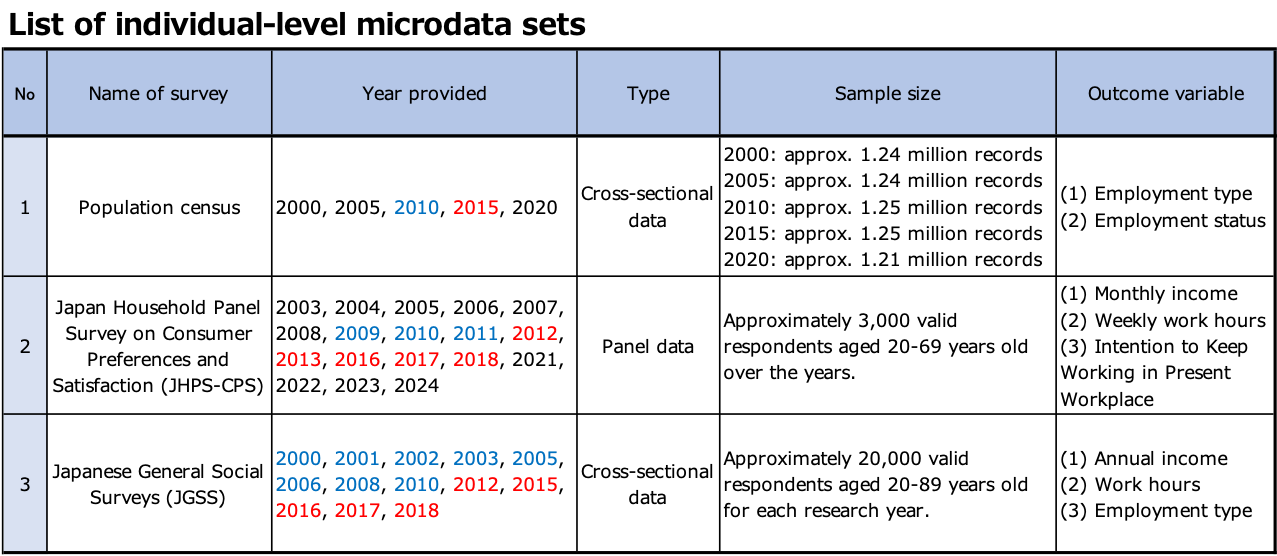
\includegraphics[width=0.93\textwidth]{list_of_individual_data.png}

  \end{figure}
\end{frame}

%---------------------------------------
% Slide: Ex. Real GRP growth rate
%---------------------------------------

\begin{frame}[label=real_GDP_growth_rate]

\frametitle{Real GRP growth rate over time: the affected prefectures (Treatment group) vs. Unaffected prefectures (Control group)}

\returnbutton{event_study_results}{Return}  % 特定のスライドにリンク

    \vspace{-0.06cm}
  \begin{figure}
    \centering
    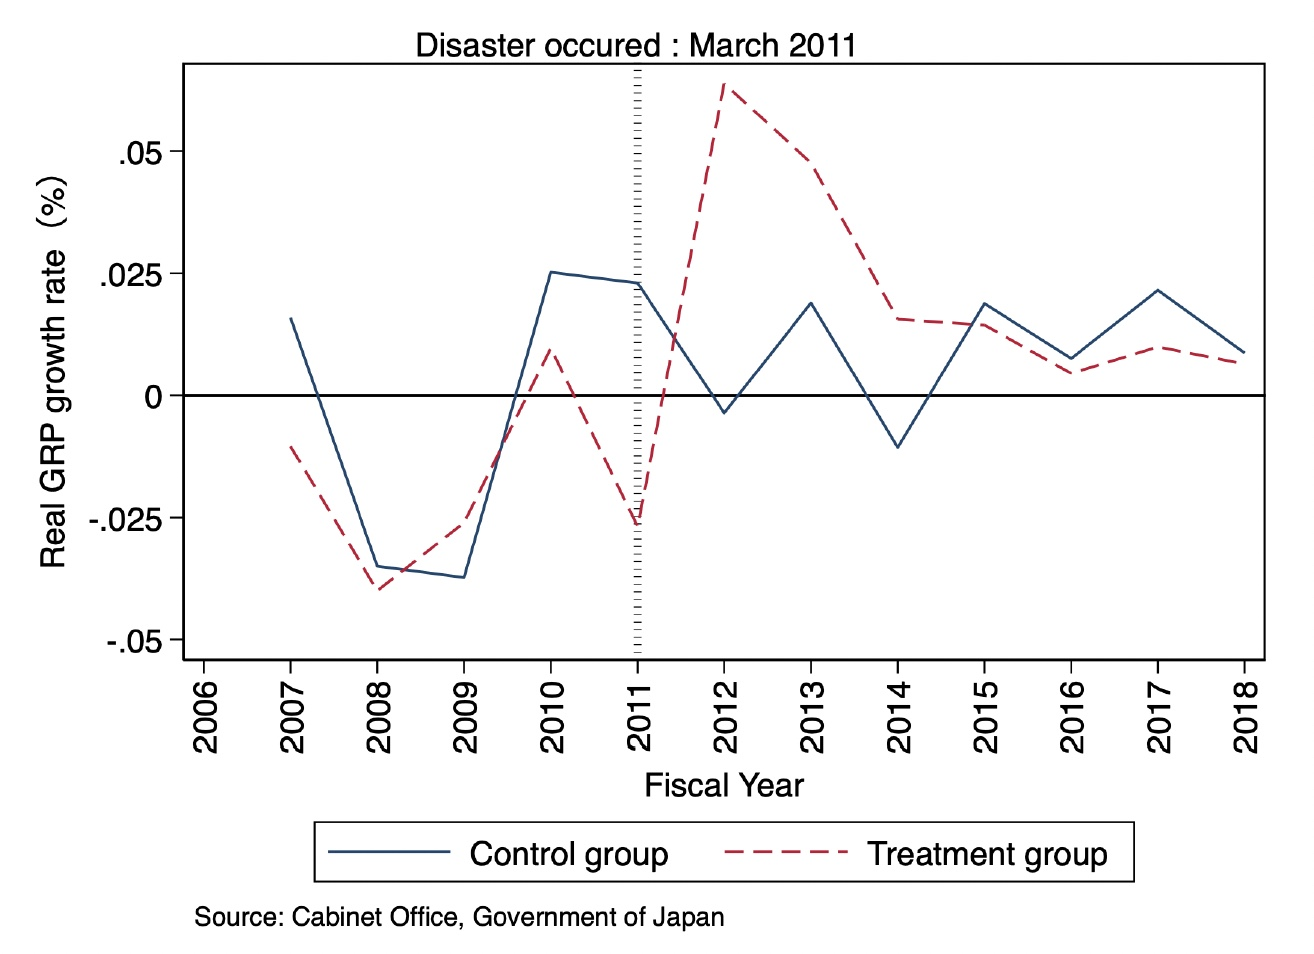
\includegraphics[width=0.62\textwidth]{Real GRP growth rate.jpeg}

  \end{figure}
\end{frame}

%%%%%%%%%%%%%%%%%%%%%%%%%%%%%%%%%%%%%%%%%

\begin{frame}[label=numbers_of_workers_full]

\vspace{0.4cm}

\returnbutton{numbers_of_workers}{Return}  % 特定のスライドにリンク

The significant
decrease in female non-regular employment may explain the substantial increase in average income for women post-disaster. (Population Census)

\vspace{-0.1cm}

\begin{table}[htbp]
\centering
\caption{Difference in the Number of Workers (2010 vs 2015) in Fukushima}
%\scriptsize
%\tiny
\scalefont{0.31}  % 0.8は倍率。必要に応じて調整してください。
\begin{tabular}{l *{9}{S[table-format=-5.0]}}
\toprule
\multirow{3}{*}{Occupation} & {\multirow{3}{*}{\makecell[c]{\textbf{Total}\\\underline{(Reg +}\\\underline{Non-reg)}}}} & \multicolumn{4}{c}{\textbf{Regular}} & \multicolumn{4}{c}{\textbf{Non-regular}} \\
\cmidrule(lr){3-6} \cmidrule(lr){7-10}
& & {\multirow{2}{*}{\makecell[c]{\underline{Regular}\\\underline{(Total)}}}} & {Regular} & {Exec.} & {Self-} & {\multirow{2}{*}{\makecell[c]{\underline{Non-reg.}\\\underline{(Total)}}}} & {Disp.} & {Part-time,} & {Family} \\
& & & {empl.} & & {empl.} & & {workers} & {temp.} & {workers} \\
\midrule
\multicolumn{10}{c}{\textbf{Male}} \\
\midrule
Total & 1289 & -545 & 10591 & -1055 & -10081 & 1834 & 870 & 2719 & -1755 \\
Admin. \& managerial & -84 & -28 & -898 & 1296 & -426 & -52 & 0 & -52 & 0 \\
Prof. \& technical & 3521 & 3186 & 3400 & -119 & -95 & 335 & 112 & 263 & -40 \\
Clerical & 9364 & 7612 & 7251 & 276 & 85 & 1752 & 828 & 925 & -1 \\
Sales & -9636 & -8513 & -5186 & -1813 & -1514 & -1123 & -29 & -692 & -402 \\
Service & -1069 & -441 & 395 & -141 & -695 & -628 & 67 & -596 & -99 \\
Security & 1184 & 1094 & 1142 & -1 & -47 & 90 & 0 & 90 & 0 \\
Agri., forest. \& fish. & -6669 & -5959 & -383 & 32 & -5608 & -710 & -16 & -6 & -688 \\
Manufacturing & -14864 & -12017 & -10002 & -614 & -1401 & -2847 & -1668 & -768 & -411 \\
Trans. \& machine op. & 1042 & 596 & 747 & 19 & -170 & 446 & 122 & 308 & 16 \\
Constr. \& mining & 13740 & 11435 & 11403 & 85 & -53 & 2319 & 0 & 2211 & 108 \\
Carrying, clean., pack. & 7279 & 4519 & 4291 & -67 & 295 & 2760 & 1657 & 1179 & -76 \\
Not Classifiable & -2569 & -2049 & -1569 & 2 & -482 & -520 & -209 & -153 & -158 \\
\midrule
\multicolumn{10}{c}{\textbf{Female}} \\
\midrule
Total & -14626 & -1518 & 208 & 24 & -1750 & -13108 & -194 & -5413 & -7501 \\
Admin. \& managerial & 141 & 173 & -131 & 337 & -33 & -14 & 0 & -14 & 0 \\
Prof. \& technical & 2629 & 1957 & 2245 & 48 & -336 & 672 & -114 & 872 & -86 \\
Clerical & 4734 & 2516 & 2034 & 384 & 98 & 2218 & 921 & 1541 & -244 \\
Sales & -6188 & -2072 & -1053 & -489 & -530 & -4116 & -184 & -2580 & -1352 \\
Service & -2922 & 284 & 1496 & -140 & -1072 & -3206 & 27 & -2359 & -874 \\
Security & -33 & 87 & 72 & 8 & 7 & -120 & 0 & -120 & 0 \\
Agri., forest. \& fish. & -3950 & -127 & 10 & -17 & -120 & -3823 & -16 & -53 & -3754 \\
Manufacturing & -8632 & -4003 & -3494 & -73 & -436 & -4629 & -765 & -3236 & -628 \\
Trans. \& machine op. & 103 & 78 & 29 & -7 & 56 & 25 & -20 & 59 & -14 \\
Constr. \& mining & 328 & 96 & 124 & -27 & -1 & 222 & 0 & 208 & 14 \\
Carrying, clean., pack. & 646 & 12 & -329 & 33 & 308 & 634 & 26 & 537 & 71 \\
Not Classifiable & -1502 & -519 & -795 & -33 & 309 & -983 & -89 & -278 & -616 \\
\bottomrule
\end{tabular}

\addlinespace[0.35em]

\raggedright
\scriptsize

\end{table}

\end{frame}
%%%%%%%%%%%%%%%%%%%%%%%%%%%%%%%%



%%%%%%%%%%%%%%%%%%%%%%%%%%%%%%%%%%%%%


\begin{frame}[label=workers_number]

\vspace{0.4cm}

\returnbutton{conclusion}{Return}  % 特定のスライドにリンク

\begin{table}[htbp]
\centering
\vspace{0.2em}
\caption{Number of workers by employment type and gender - Fukushima, Nationwide}

\resizebox{\textwidth}{!}{%
\begin{tabular}{lllllllllll}
\hline
\multirow{2}{*}{} & \multirow{2}{*}{\makecell[l]{Survey\\Year}} & \multirow{2}{*}{\makecell[l]{Total\\population}} & \multirow{2}{*}{\makecell[l]{Population of\\working age}} & \multirow{2}{*}{\makecell[l]{Total\\workers}} & \multirow{2}{*}{\makecell[l]{Regular\\employees}} & \multirow{2}{*}{\makecell[l]{Executives}} & \multirow{2}{*}{\makecell[l]{Self-\\employed}} & \multirow{2}{*}{\makecell[l]{Dispatched\\workers}} & \multirow{2}{*}{\makecell[l]{Part-time\\workers}} & \multirow{2}{*}{\makecell[l]{Family\\workers}} \\
 &  &  &  &  &  &  &  &  &  & \\
\hline
\addlinespace[0.5em]
\multicolumn{11}{l}{\textbf{Fukushima Pref}} \\
\addlinespace[0.5em]
Male & 2010 & 984,682 & 835,901 & \multicolumn{1}{l}{523,911} & \multicolumn{1}{l}{331,909} & \multicolumn{1}{l}{35,545} & \multicolumn{1}{l}{80,671} & \multicolumn{1}{l}{11,810} & \multicolumn{1}{l}{52,081} & \multicolumn{1}{l}{11,895} \\
 & 2015 & 945,660 (-4.0\%) & 813,542 (-2.7\%) & \multicolumn{1}{l}{525,200 (0.2\%)} & \multicolumn{1}{l}{342,500 (3.2\%)} & \multicolumn{1}{l}{34,490 (-3.0\%)} & \multicolumn{1}{l}{70,590 (-12.5\%)} & \multicolumn{1}{l}{12,680 (7.4\%)} & \multicolumn{1}{l}{54,800 (5.2\%)} & \multicolumn{1}{l}{10,140 (-14.8\%)} \\
 & 2020 & 903,864 (-8.2\%) & 777,758 (-6.9\%) & \multicolumn{1}{l}{477,770 (-8.8\%)} & \multicolumn{1}{l}{313,760 (-5.5\%)} & \multicolumn{1}{l}{35,330 (-0.6\%)} & \multicolumn{1}{l}{62,420 (-22.6\%)} & \multicolumn{1}{l}{10,040 (-15.0\%)} & \multicolumn{1}{l}{48,640 (-6.6\%)} & \multicolumn{1}{l}{7,580 (-36.3\%)} \\
\addlinespace[0.3em]
Female & 2010 & 1,044,382 & 905,008 & \multicolumn{1}{l}{400,036} & \multicolumn{1}{l}{162,482} & \multicolumn{1}{l}{12,336} & \multicolumn{1}{l}{21,410} & \multicolumn{1}{l}{12,224} & \multicolumn{1}{l}{148,763} & \multicolumn{1}{l}{42,821} \\
 & 2015 & 968,379 (-7.3\%) & 849,031 (-6.2\%) & \multicolumn{1}{l}{385,410 (-3.7\%)} & \multicolumn{1}{l}{162,690 (0.1\%)} & \multicolumn{1}{l}{12,360 (0.2\%)} & \multicolumn{1}{l}{19,660 (-8.2\%)} & \multicolumn{1}{l}{12,030 (-1.6\%)} & \multicolumn{1}{l}{143,350 (-3.6\%)} & \multicolumn{1}{l}{35,320 (-17.5\%)} \\
 & 2020 & 929,288 (-11.0\%) & 815,308 (-9.9\%) & \multicolumn{1}{l}{371,830 (-7.1\%)} & \multicolumn{1}{l}{166,900 (2.7\%)} & \multicolumn{1}{l}{12,320 (-0.1\%)} & \multicolumn{1}{l}{18,130 (-15.3\%)} & \multicolumn{1}{l}{10,430 (-14.7\%)} & \multicolumn{1}{l}{134,950 (-9.3\%)} & \multicolumn{1}{l}{29,100 (-32.0\%)} \\
\hline
\addlinespace[0.5em]
\multicolumn{11}{l}{\textbf{Nationwide}} \\
\addlinespace[0.5em]
Male & 2010 & 62,327,737 & 53,154,614 & \multicolumn{1}{l}{32,738,782} & \multicolumn{1}{l}{21,002,407} & \multicolumn{1}{l}{2,433,694} & \multicolumn{1}{l}{4,291,165} & \multicolumn{1}{l}{639,470} & \multicolumn{1}{l}{3,883,461} & \multicolumn{1}{l}{488,585} \\
 & 2015 & 61,841,738 (-0.8\%) & 52,879,791 (-0.5\%) & \multicolumn{1}{l}{31,720,790 (-3.1\%)} & \multicolumn{1}{l}{20,536,000 (-2.2\%)} & \multicolumn{1}{l}{2,213,220 (-9.1\%)} & \multicolumn{1}{l}{3,959,660 (-7.7\%)} & \multicolumn{1}{l}{652,830 (2.1\%)} & \multicolumn{1}{l}{3,942,620 (1.5\%)} & \multicolumn{1}{l}{416,460 (-14.8\%)} \\
 & 2020 & 61,349,581 (-1.6\%) & 52,098,467 (-2.0\%) & \multicolumn{1}{l}{30,871,667 (-5.7\%)} & \multicolumn{1}{l}{20,065,078 (-4.5\%)} & \multicolumn{1}{l}{2,364,280 (-2.9\%)} & \multicolumn{1}{l}{3,600,577 (-16.1\%)} & \multicolumn{1}{l}{638,324 (-0.2\%)} & \multicolumn{1}{l}{3,877,779 (-0.1\%)} & \multicolumn{1}{l}{325,629 (-33.4\%)} \\
\addlinespace[0.3em]
Female & 2010 & 65,729,615 & 57,122,871 & \multicolumn{1}{l}{24,627,898} & \multicolumn{1}{l}{9,433,752} & \multicolumn{1}{l}{746,640} & \multicolumn{1}{l}{1,286,990} & \multicolumn{1}{l}{891,120} & \multicolumn{1}{l}{10,436,445} & \multicolumn{1}{l}{1,832,951} \\
 & 2015 & 65,253,007 (-0.7\%) & 56,874,386 (-0.4\%) & \multicolumn{1}{l}{24,914,620 (1.2\%)} & \multicolumn{1}{l}{9,729,320 (3.1\%)} & \multicolumn{1}{l}{711,090 (-4.8\%)} & \multicolumn{1}{l}{1,247,870 (-3.0\%)} & \multicolumn{1}{l}{880,160 (-1.2\%)} & \multicolumn{1}{l}{10,795,720 (3.4\%)} & \multicolumn{1}{l}{1,550,460 (-15.4\%)} \\
 & 2020 & 64,796,518 (-1.4\%) & 56,160,102 (-1.7\%) & \multicolumn{1}{l}{25,675,371 (4.3\%)} & \multicolumn{1}{l}{10,731,753 (13.8\%)} & \multicolumn{1}{l}{769,919 (3.1\%)} & \multicolumn{1}{l}{1,264,299 (-1.8\%)} & \multicolumn{1}{l}{883,817 (-0.8\%)} & \multicolumn{1}{l}{10,745,470 (3.0\%)} & \multicolumn{1}{l}{1,280,113 (-30.2\%)} \\
\hline
\end{tabular}%
}
\addlinespace[0.12em]
\raggedright
\scriptsize
\textit{Note}: "Total workers" represent the number of workers in the population of working age (15 years and over) by gender for Fukushima Prefecture and Japan as a whole. Workers with "employment type not classifiable" are not included in the table and are excluded from the Total workers count. Percentages in parentheses represent the growth rate compared to the number of workers in 2010.\\
\textit{Source}: 2010, 2015 and 2020 Population Census.\\
\label{table:Number_of_workers}
\end{table}

\end{frame}

%%%%%%%%%%%%%%%%%%%%%%%%%%%%%%

\begin{frame}[fragile,label=appendix1]

\vspace{0.40cm} 
\returnbutton{proportion_of_employment_type}{Return}

\vspace{-0.30cm} 

\begin{figure}
\centering
\resizebox{0.96\textwidth}{!}{
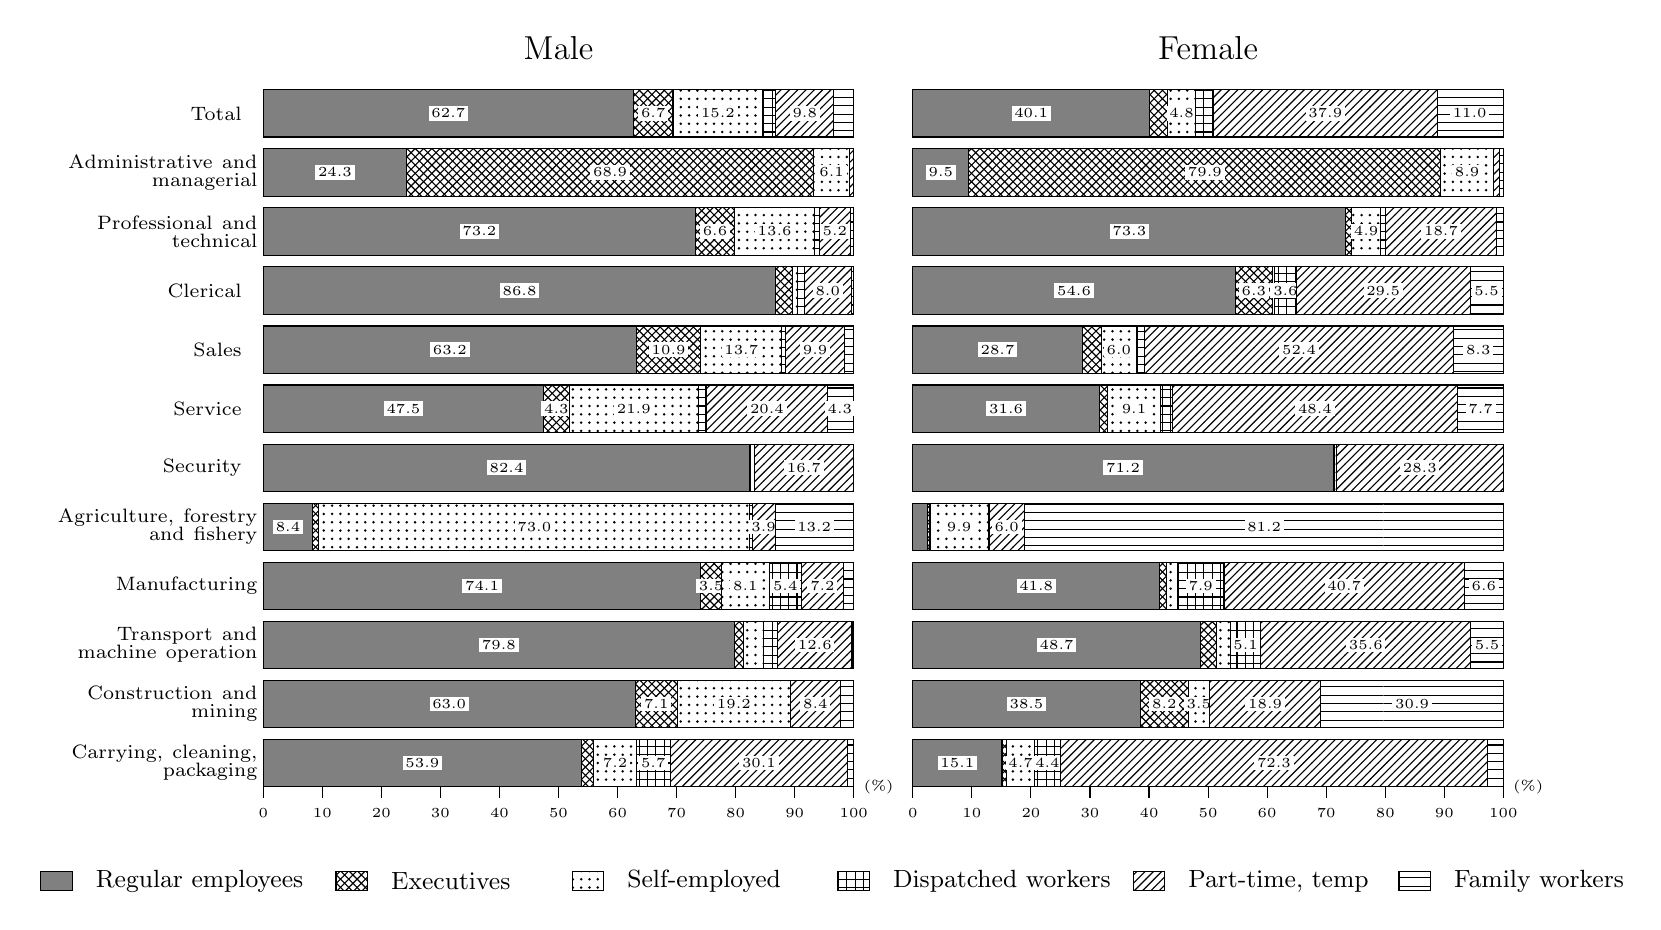
\begin{tikzpicture}[scale=0.75,xshift=-0.5cm]

% Define Colors
\definecolor{color1}{RGB}{128,128,128}
\definecolor{color2}{RGB}{200,200,200}
\definecolor{color3}{RGB}{220,220,220}
\definecolor{color4}{RGB}{180,180,180}
\definecolor{color5}{RGB}{100,100,100}
\definecolor{color6}{RGB}{60,60,60}

% Function to draw a stacked bar
\newcommand{\stackedbar}[8]{%
    \draw[fill=color1] (#1,#2) rectangle (#1+#3/10,#2+0.8);
    \pgfmathtruncatemacro{\resultA}{int(#3 >= 3.5 ? 1 : 0)}
    \ifnum\resultA>0
        \node[font=\tiny,fill=white,text=black,inner sep=1pt] at (#1+#3/20,#2+0.4) {#3};
    \fi
    \draw[fill=color2, pattern=crosshatch] (#1+#3/10,#2) rectangle (#1+#3/10+#4/10,#2+0.8);
    \pgfmathtruncatemacro{\resultB}{int(#4 >= 3.5 ? 1 : 0)}
    \ifnum\resultB>0
        \node[font=\tiny,fill=white,text=black,inner sep=1pt] at (#1+#3/10+#4/20,#2+0.4) {#4};
    \fi
    \draw[fill=color3, pattern=dots] (#1+#3/10+#4/10,#2) rectangle (#1+#3/10+#4/10+#5/10,#2+0.8);
    \pgfmathtruncatemacro{\resultC}{int(#5 >= 3.5 ? 1 : 0)}
    \ifnum\resultC>0
        \node[font=\tiny,fill=white,text=black,inner sep=1pt] at (#1+#3/10+#4/10+#5/20,#2+0.4) {#5};
    \fi
    \draw[fill=color4, pattern=grid] (#1+#3/10+#4/10+#5/10,#2) rectangle (#1+#3/10+#4/10+#5/10+#6/10,#2+0.8);
    \pgfmathtruncatemacro{\resultD}{int(#6 >= 3.5 ? 1 : 0)}
    \ifnum\resultD>0
        \node[font=\tiny,fill=white,text=black,inner sep=1pt] at (#1+#3/10+#4/10+#5/10+#6/20,#2+0.4) {#6};
    \fi
    \draw[fill=color5, pattern=north east lines] (#1+#3/10+#4/10+#5/10+#6/10,#2) rectangle (#1+#3/10+#4/10+#5/10+#6/10+#7/10,#2+0.8);
    \pgfmathtruncatemacro{\resultE}{int(#7 >= 3.5 ? 1 : 0)}
    \ifnum\resultE>0
        \node[font=\tiny,fill=white,text=black,inner sep=1pt] at (#1+#3/10+#4/10+#5/10+#6/10+#7/20,#2+0.4) {#7};
    \fi
    \draw[fill=color6, pattern=horizontal lines] (#1+#3/10+#4/10+#5/10+#6/10+#7/10,#2) rectangle (#1+10,#2+0.8);
    \pgfmathtruncatemacro{\resultF}{int(#8 >= 3.5 ? 1 : 0)}
    \ifnum\resultF>0
        \node[font=\tiny,fill=white,text=black,inner sep=1pt] at (#1+#3/10+#4/10+#5/10+#6/10+#7/10+#8/20,#2+0.4) {#8};
    \fi
}

% Male bars
\begin{scope}[xshift=-5.5cm]
    \stackedbar{0}{11}{62.7}{6.7}{15.2}{2.2}{9.8}{2.3}
    \node[anchor=east, text width=2.6cm, align=right] at (-0.2,11.4) {\scriptsize Total};
    
    \stackedbar{0}{10}{24.3}{68.9}{6.1}{0}{0.7}{0}
    \node[anchor=east, text width=2.6cm, align=right] at (-0.2,10.4) {\scriptsize\parbox[t]{2.8cm}{\setstretch{0.8}\raggedleft Administrative and managerial}};
    
    \stackedbar{0}{9}{73.2}{6.6}{13.6}{0.8}{5.2}{0.6}
    \node[anchor=east, text width=2.6cm, align=right] at (-0.2,9.4) {\scriptsize\parbox[t]{2.8cm}{\setstretch{0.8}\raggedleft Professional and technical}};
    
    \stackedbar{0}{8}{86.8}{2.9}{0.7}{1.2}{8.0}{0.3}
    \node[anchor=east, text width=2.6cm, align=right] at (-0.2,8.4) {\scriptsize Clerical};
    
    \stackedbar{0}{7}{63.2}{10.9}{13.7}{0.7}{9.9}{1.6}
    \node[anchor=east, text width=2.6cm, align=right] at (-0.2,7.4) {\scriptsize Sales};
    
    \stackedbar{0}{6}{47.5}{4.3}{21.9}{1.4}{20.4}{4.3}
    \node[anchor=east, text width=2.6cm, align=right] at (-0.2,6.4) {\scriptsize Service};
    
    \stackedbar{0}{5}{82.4}{0.1}{0.7}{0}{16.7}{0}
    \node[anchor=east, text width=2.6cm, align=right] at (-0.2,5.4) {\scriptsize Security};
    
    \stackedbar{0}{4}{8.4}{1.0}{73.0}{0.4}{3.9}{13.2}
    \node[anchor=east, text width=2.6cm, align=right] at (-0.2,4.4) {\scriptsize\parbox[t]{2.8cm}{\setstretch{0.8}\raggedleft Agriculture, forestry and fishery}};
    
    \stackedbar{0}{3}{74.1}{3.5}{8.1}{5.4}{7.2}{1.5}
    \node[anchor=east, text width=2.6cm, align=right] at (-0.2,3.4) {\scriptsize\parbox[t]{2.8cm}{\setstretch{0.8}\raggedleft Manufacturing}};
    
    \stackedbar{0}{2}{79.8}{1.5}{3.4}{2.4}{12.6}{0.2}
    \node[anchor=east, text width=2.6cm, align=right] at (-0.2,2.4) {\scriptsize\parbox[t]{2.8cm}{\setstretch{0.8}\raggedleft Transport and machine operation}};
    
    \stackedbar{0}{1}{63.0}{7.1}{19.2}{0}{8.4}{2.2}
    \node[anchor=east, text width=2.6cm, align=right] at (-0.2,1.4) {\scriptsize\parbox[t]{2.8cm}{\setstretch{0.8}\raggedleft Construction and mining}};
    
    \stackedbar{0}{0}{53.9}{2.1}{7.2}{5.7}{30.1}{1.0}
    \node[anchor=east, text width=2.6cm, align=right] at (-0.2,0.4) {\scriptsize\parbox[t]{2.8cm}{\setstretch{0.8}\raggedleft Carrying, cleaning, packaging}};
    
    % X-axis for Male
    \draw (0,0) -- (10,0);
    \foreach \x in {0,1,...,10} {
        \draw (\x,0) -- (\x,-0.2) 
            node[anchor=north] {\tiny \ifnum\x=0 0\else\x0\fi};
    }
    \node[anchor=west] at (10,0) {\tiny (\%)};
    
    % Label for Male
    \node[anchor=center] at (5,12.5) {\large Male};
\end{scope}

% Female bars
\begin{scope}[xshift=5.5cm]
    \stackedbar{0}{11}{40.1}{3.0}{4.8}{3.0}{37.9}{11.0}
    \stackedbar{0}{10}{9.5}{79.9}{8.9}{0}{1.1}{0.6}
    \stackedbar{0}{9}{73.3}{1.0}{4.9}{0.9}{18.7}{1.2}
    \stackedbar{0}{8}{54.6}{6.3}{0.4}{3.6}{29.5}{5.5}
    \stackedbar{0}{7}{28.7}{3.2}{6.0}{1.3}{52.4}{8.3}
    \stackedbar{0}{6}{31.6}{1.3}{9.1}{1.9}{48.4}{7.7}
    \stackedbar{0}{5}{71.2}{0.2}{0.3}{0}{28.3}{0}
    \stackedbar{0}{4}{2.5}{0.4}{9.9}{0.1}{6.0}{81.2}
    \stackedbar{0}{3}{41.8}{1.1}{1.9}{7.9}{40.7}{6.6}
    \stackedbar{0}{2}{48.7}{2.7}{2.4}{5.1}{35.6}{5.5}
    \stackedbar{0}{1}{38.5}{8.2}{3.5}{0}{18.9}{30.9}
    \stackedbar{0}{0}{15.1}{0.8}{4.7}{4.4}{72.3}{2.8}
    
    % X-axis for Female
    \draw (0,0) -- (10,0);
    \foreach \x in {0,1,...,10} {
        \draw (\x,0) -- (\x,-0.2) 
            node[anchor=north] {\tiny \ifnum\x=0 0\else\x0\fi};
    }
    \node[anchor=west] at (10,0) {\tiny (\%)};
    
    % Label for Female
    \node[anchor=center] at (5,12.5) {\large Female};
\end{scope}

\vspace{-0.50cm} 

% Legend (1 row, 6 columns)
\node[anchor=center, fill=color1, minimum width=0.4cm, minimum height=0.2cm, draw] at (-9,-1.6) {};
\node[anchor=west] at (-8.5,-1.6) {\small Regular employees};
\node[anchor=center, fill=color2, pattern=crosshatch, minimum width=0.4cm, minimum height=0.2cm, draw] at (-4,-1.6) {};
\node[anchor=west] at (-3.5,-1.6) {\small Executives};
\node[anchor=center, fill=color3, pattern=dots, minimum width=0.4cm, minimum height=0.2cm, draw] at (0,-1.6) {};
\node[anchor=west] at (0.5,-1.6) {\small Self-employed};
\node[anchor=center, fill=color4, pattern=grid, minimum width=0.4cm, minimum height=0.2cm, draw] at (4.5,-1.6) {};
\node[anchor=west] at (5,-1.6) {\small Dispatched workers};
\node[anchor=center, fill=color5, pattern=north east lines, minimum width=0.4cm, minimum height=0.2cm, draw] at (9.5,-1.6) {};
\node[anchor=west] at (10,-1.6) {\small Part-time, temp};
\node[anchor=center, fill=color6, pattern=horizontal lines, minimum width=0.4cm, minimum height=0.2cm, draw] at (14,-1.6) {};
\node[anchor=west] at (14.5,-1.6) {\small Family workers};


\end{tikzpicture}
}
%\caption{Proportion of Employed Persons Aged 15 and Over by Occupation, Employment types, and Gender - Fukushima Prefecture (2010)}
\end{figure}

\end{frame}

%%%%%%%%%%%%%%%%%%%%%%%%%%%%%%%%%%%%%%%%%%


\begin{frame}[label=appendix2]

\frametitle{Proportion of Employed Persons by Industry - Fukushima (2010)}

\vspace{0.20cm} 

\returnbutton{proportion_of_employment_type}{Return}  % 特定のスライドにリンク

\begin{figure}[htbp]
    \centering 
    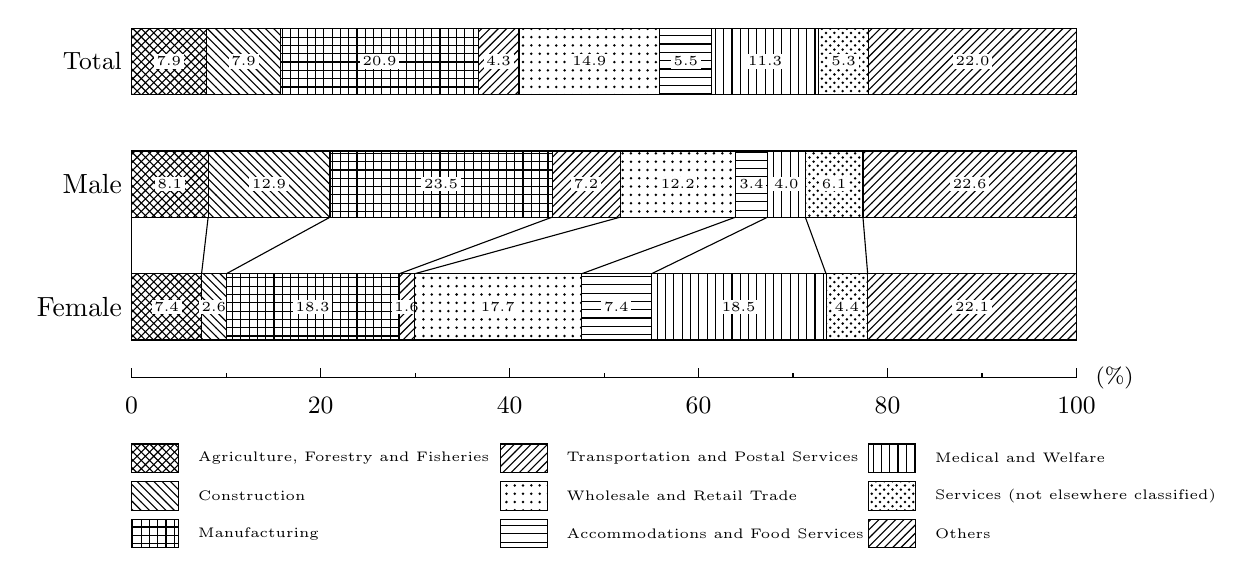
\begin{tikzpicture}[scale=1.20]
    % 色の定義
    \definecolor{color1}{RGB}{200,200,200} 
    \definecolor{color2}{RGB}{150,150,150} 
    \definecolor{color3}{RGB}{100,100,100}
    \definecolor{color4}{RGB}{250,200,200}
    \definecolor{color5}{RGB}{200,150,150}
    \definecolor{color6}{RGB}{150,100,100}
    \definecolor{color7}{RGB}{100,50,50}
    \definecolor{color8}{RGB}{50,0,0}
    \definecolor{color9}{RGB}{0,0,0}
    
    % 棒グラフの描画
    % Total bar
    \draw[fill=color1, pattern=crosshatch] (2,9) rectangle (2.79,9.7) node[pos=0.5, fill=white, inner sep=1pt] {\tiny 7.9};
    \draw[fill=color2, pattern=north west lines] (2.79,9) rectangle (3.58,9.7) node[pos=0.5, fill=white, inner sep=1pt] {\tiny 7.9};
    \draw[fill=color3, pattern=grid] (3.58,9) rectangle (5.67,9.7) node[pos=0.5, fill=white, inner sep=1pt] {\tiny 20.9};
    \draw[fill=color4, pattern=north east lines] (5.67,9) rectangle (6.10,9.7) node[pos=0.5, fill=white, inner sep=1pt] {\tiny 4.3}; 
    \draw[fill=color5, pattern=dots] (6.10,9) rectangle (7.59,9.7) node[pos=0.5, fill=white, inner sep=1pt] {\tiny 14.9}; 
    \draw[fill=color6, pattern=horizontal lines] (7.59,9) rectangle (8.14,9.7) node[pos=0.5, fill=white, inner sep=1pt] {\tiny 5.5};
    \draw[fill=color7, pattern=vertical lines] (8.14,9) rectangle (9.27,9.7) node[pos=0.5, fill=white, inner sep=1pt] {\tiny 11.3};
    \draw[fill=color8, pattern=crosshatch dots] (9.27,9) rectangle (9.80,9.7) node[pos=0.5, fill=white, inner sep=1pt] {\tiny 5.3};
    \draw[fill=color9, pattern=north east lines] (9.80,9) rectangle (12,9.7) node[pos=0.5, fill=white, inner sep=1pt] {\tiny 22.0}; 
    
    % Male bar
    \draw[fill=color1, pattern=crosshatch] (2,7.7) rectangle (2.81,8.4) node[pos=0.5, fill=white, inner sep=1pt] {\tiny 8.1};
    \draw[fill=color2, pattern=north west lines] (2.81,7.7) rectangle (4.10,8.4) node[pos=0.5, fill=white, inner sep=1pt] {\tiny 12.9};
    \draw[fill=color3, pattern=grid] (4.10,7.7) rectangle (6.45,8.4) node[pos=0.5, fill=white, inner sep=1pt] {\tiny 23.5};
    \draw[fill=color4, pattern=north east lines] (6.45,7.7) rectangle (7.17,8.4) node[pos=0.5, fill=white, inner sep=1pt] {\tiny 7.2}; 
    \draw[fill=color5, pattern=dots] (7.17,7.7) rectangle (8.39,8.4) node[pos=0.5, fill=white, inner sep=1pt] {\tiny 12.2}; 
    \draw[fill=color6, pattern=horizontal lines] (8.39,7.7) rectangle (8.73,8.4) node[pos=0.5, fill=white, inner sep=1pt] {\tiny 3.4};
    \draw[fill=color7, pattern=vertical lines] (8.73,7.7) rectangle (9.13,8.4) node[pos=0.5, fill=white, inner sep=1pt] {\tiny 4.0};
    \draw[fill=color8, pattern=crosshatch dots] (9.13,7.7) rectangle (9.74,8.4) node[pos=0.5, fill=white, inner sep=1pt] {\tiny 6.1};
    \draw[fill=color9, pattern=north east lines] (9.74,7.7) rectangle (12,8.4) node[pos=0.5, fill=white, inner sep=1pt] {\tiny 22.6};
    
    % Female bar
    \draw[fill=color1, pattern=crosshatch] (2,6.4) rectangle (2.74,7.1) node[pos=0.5, fill=white, inner sep=1pt] {\tiny 7.4};
    \draw[fill=color2, pattern=north west lines] (2.74,6.4) rectangle (3.00,7.1) node[pos=0.5, fill=white, inner sep=1pt] {\tiny 2.6};
    \draw[fill=color3, pattern=grid] (3.00,6.4) rectangle (4.83,7.1) node[pos=0.5, fill=white, inner sep=1pt] {\tiny 18.3};
    \draw[fill=color4, pattern=north east lines] (4.83,6.4) rectangle (4.99,7.1) node[pos=0.5, fill=white, inner sep=1pt] {\tiny 1.6}; 
    \draw[fill=color5, pattern=dots] (4.99,6.4) rectangle (6.76,7.1) node[pos=0.5, fill=white, inner sep=1pt] {\tiny 17.7}; 
    \draw[fill=color6, pattern=horizontal lines] (6.76,6.4) rectangle (7.50,7.1) node[pos=0.5, fill=white, inner sep=1pt] {\tiny 7.4};
    \draw[fill=color7, pattern=vertical lines] (7.50,6.4) rectangle (9.35,7.1) node[pos=0.5, fill=white, inner sep=1pt] {\tiny 18.5};
    \draw[fill=color8, pattern=crosshatch dots] (9.35,6.4) rectangle (9.79,7.1) node[pos=0.5, fill=white, inner sep=1pt] {\tiny 4.4};
    \draw[fill=color9, pattern=north east lines] (9.79,6.4) rectangle (12,7.1) node[pos=0.5, fill=white, inner sep=1pt] {\tiny 22.1}; 
    
    % ガイドラインの描画(Maleのバーの下端から対応するFemaleのバーの上端へ)
    \draw[thin] (2.00,7.7) -- (2.00,7.1);    % Agriculture, left
    \draw[thin] (2.81,7.7) -- (2.74,7.1);    % Agriculture, right
    \draw[thin] (4.10,7.7) -- (3.00,7.1);    % Construction
    \draw[thin] (6.45,7.7) -- (4.83,7.1);    % Manufacturing
    \draw[thin] (7.17,7.7) -- (4.99,7.1);    % Wholesale and Retail Trade, left
    \draw[thin] (8.39,7.7) -- (6.76,7.1);    % Wholesale and Retail Trade, right
    \draw[thin] (8.73,7.7) -- (7.50,7.1);    % Accommodations and Food Services, right
    \draw[thin] (9.13,7.7) -- (9.35,7.1);    % Medical and Welfare
    \draw[thin] (9.74,7.7) -- (9.79,7.1);    % Services (not elsewhere classified)
    \draw[thin] (12,7.7) -- (12,7.1);        % Others
    
    % ラベルの描画(フォントサイズを調整)
    \node[anchor=east, font=\small] at (2,9.35) {Total};
    \node[anchor=east, font=\normalsize] at (2,8.05) {Male};
    \node[anchor=east, font=\normalsize] at (2,6.75) {Female};
    
    % X軸の描画
    \draw (2,6) -- (12,6);
    \foreach \x in {0,20,40,60,80,100} {
        \draw (2+\x/10,6) -- (2+\x/10,6.1) 
            node[anchor=north] at (2+\x/10,5.9) {\small \x};
    }
    \foreach \x in {10,30,50,70,90} {
        \draw (2+\x/10,6) -- (2+\x/10,6.05);
    }
    \node[anchor=west, font=\footnotesize] at (12.1,6) {(\%)};
    
    % 凡例の描画(手動で作成)
    \begin{scope}[shift={(0,5.0)}] % 凡例の位置を調整
        % 列間の間隔を1.3倍に拡大(x=2, 5.9, 9.8)
        
        % 列1
        \draw[fill=color1, pattern=crosshatch, minimum width=0.5cm, minimum height=0.3cm, draw] (2,0) rectangle ++(0.5,0.3);
        \node[anchor=west, font=\tiny] at (2.6,0.15) {Agriculture, Forestry and Fisheries};
        
        \draw[fill=color2, pattern=north west lines, minimum width=0.5cm, minimum height=0.3cm, draw] (2,-0.4) rectangle ++(0.5,0.3);
        \node[anchor=west, font=\tiny] at (2.6,-0.25) {Construction};
        
        \draw[fill=color3, pattern=grid, minimum width=0.5cm, minimum height=0.3cm, draw] (2,-0.8) rectangle ++(0.5,0.3);
        \node[anchor=west, font=\tiny] at (2.6,-0.65) {Manufacturing};
        
        % 列2 (x=5.9)
        \draw[fill=color4, pattern=north east lines, minimum width=0.5cm, minimum height=0.3cm, draw] (5.9,0) rectangle ++(0.5,0.3);
        \node[anchor=west, font=\tiny] at (6.5,0.15) {Transportation and Postal Services};
        
        \draw[fill=color5, pattern=dots, minimum width=0.5cm, minimum height=0.3cm, draw] (5.9,-0.4) rectangle ++(0.5,0.3);
        \node[anchor=west, font=\tiny] at (6.5,-0.25) {Wholesale and Retail Trade};
        
        \draw[fill=color6, pattern=horizontal lines, minimum width=0.5cm, minimum height=0.3cm, draw] (5.9,-0.8) rectangle ++(0.5,0.3);
        \node[anchor=west, font=\tiny] at (6.5,-0.65) {Accommodations and Food Services};
        
        % 列3 (x=9.8)
        \draw[fill=color7, pattern=vertical lines, minimum width=0.5cm, minimum height=0.3cm, draw] (9.8,0) rectangle ++(0.5,0.3);
        \node[anchor=west, font=\tiny] at (10.4,0.15) {Medical and Welfare};
        
        \draw[fill=color8, pattern=crosshatch dots, minimum width=0.5cm, minimum height=0.3cm, draw] (9.8,-0.4) rectangle ++(0.5,0.3);
        \node[anchor=west, font=\tiny] at (10.4,-0.25) {Services (not elsewhere classified)};
        
        \draw[fill=color9, pattern=north east lines, minimum width=0.5cm, minimum height=0.3cm, draw] (9.8,-0.8) rectangle ++(0.5,0.3);
        \node[anchor=west, font=\tiny] at (10.4,-0.65) {Others};
    \end{scope}
    
    \end{tikzpicture} 
    % \caption{Proportion of Employed Persons Aged 15 and Over by Industry and Sex - Fukushima (2010)} % \captionを削除
\end{figure}

\end{frame}


%%%%%%%%%%%%%%%%%%%%%%%%%%%%%%%%%%%%%%%%%%%
%Gender Gap Index (GGI) 2024
%%%%%%%%%%%%%%%%%%%%%%%%%%%%%%%%%%%%%%%%%%%

\begin{frame}[label=gendergapindex]
\frametitle{Gender Gap Index (GGI), World Economic Forum 2024}

\vspace{0.2cm} 
\returnbutton{gender_income_gap}{Return}

\vspace{-0.3cm}

    \begin{figure}
        \centering
        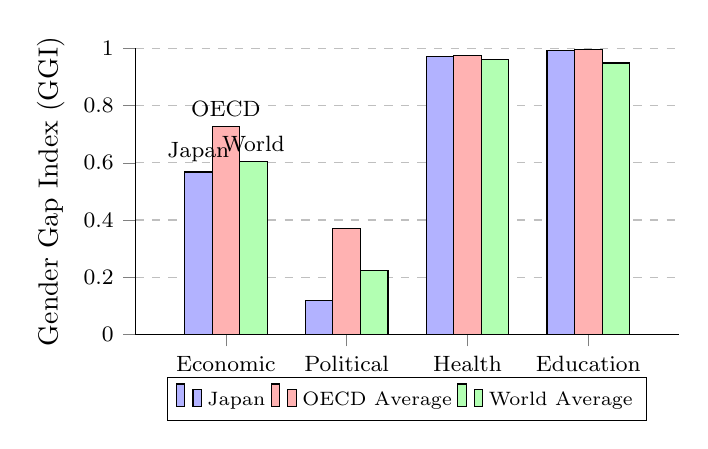
\begin{tikzpicture}
            \begin{axis}[
                ybar,
                bar width=0.35cm,
                width=0.7\textwidth,
                height=0.43\textwidth,
                enlarge x limits=0.25,
                symbolic x coords={Economic, Political, Health, Education},
                xtick=data,
                ymin=0, ymax=1,
                ylabel={Gender Gap Index (GGI)},
                ymajorgrids=true,
                grid style=dashed,
                enlarge y limits=0,
                axis x line*=bottom,
                axis y line*=left,
                tick align=outside,
                x tick label style={font=\footnotesize},
                y tick label style={font=\footnotesize},
                legend style={
                    at={(0.5,-0.15)},
                    anchor=north,
                    legend columns=3,
                    font=\scriptsize, % フォントサイズを一段階小さく
                },
            ]
            % Japan
            \addplot[
                pattern=north east lines,
                pattern color=blue,
                fill=blue!30,
                bar shift=-0.35cm, % 左にシフト
            ] coordinates {
                (Economic,0.568)
                (Political,0.118)
                (Health,0.973)
                (Education,0.993)
            };
            % OECD Average
            \addplot[
                pattern=crosshatch,
                pattern color=red,
                fill=red!30,
                bar shift=0cm, % 中央にシフトなし
            ] coordinates {
                (Economic,0.728)
                (Political,0.372)
                (Health,0.974)
                (Education,0.995)
            };
            % World Average
            \addplot[
                pattern=dots,
                pattern color=green,
                fill=green!30,
                bar shift=0.35cm, % 右にシフト
            ] coordinates {
                (Economic,0.605)
                (Political,0.225)
                (Health,0.960)
                (Education,0.949)
            };
            
            % ラベルの配置
            % 日本のEconomicバー
            \node[font=\footnotesize, above, xshift=-0.35cm] at (axis cs:Economic,0.568) {Japan};
            % OECD平均のEconomicバー
            \node[font=\footnotesize, above] at (axis cs:Economic,0.728) {OECD};
            % 世界平均のEconomicバー
            \node[font=\footnotesize, above, xshift=0.35cm] at (axis cs:Economic,0.605) {World};
            
            % 凡例の追加
            \vspace{-0.2cm}
            \legend{Japan, OECD Average, World Average}
            \end{axis}
        \end{tikzpicture}

    \vspace{-0.1cm}
    \small Japan ranks 104th out of 146 countries in the 2024 Gender Gap Index. While scoring high in education and health, it lags significantly in economic participation and political empowerment.
    \end{figure}
\end{frame}

%%%%%%%%%%%%%%%%%%%%%%%%%%%%%%%%
%Income Bands by Gender
%%%%%%%%%%%%%%%%%%%%%%%%%%%%%%%%

\begin{frame}[label=income_band]
\frametitle{Income Bands by Gender: Pre- (2000-2010) vs Post-Disaster (2012-2018) Analysis (JGSS)}
\vspace{-0.4cm}
\returnbutton{income_band_main}{Return}
    \vspace{0.01cm}
    \begin{columns}[T]
        \begin{column}{0.7\textwidth}
            \raggedright
            \begin{table}
                \tiny
                \setlength{\tabcolsep}{1.2pt}
                \renewcommand{\arraystretch}{0.8}
                \begin{tabular}{lcccccccccccccc}
                    \toprule
                    & \multicolumn{14}{c}{Survey Year} \\
                    \cmidrule(lr){2-15}
                    Area & \quad \textcolor{blue}{2000} & \textcolor{blue}{2001} & \textcolor{blue}{2002} & \textcolor{blue}{2003} & \textcolor{blue}{2005} & \textcolor{blue}{2006} & \textcolor{blue}{2008} & \textcolor{blue}{2010} & \textcolor{red}{2012} & \textcolor{red}{2015} & \textcolor{red}{2016} & \textcolor{red}{2017} & \textcolor{red}{2018} & \quad Total\\
                    \midrule
                    Non-disaster area & \quad \textcolor{blue}{2,753} & \textcolor{blue}{2,664} & \textcolor{blue}{2,812} & \textcolor{blue}{3,462} & \textcolor{blue}{1,943} & \textcolor{blue}{4,084} & \textcolor{blue}{4,009} & \textcolor{blue}{4,772} & \textcolor{red}{4,461} & \textcolor{red}{1,976} & \textcolor{red}{922} & \textcolor{red}{714} & \textcolor{red}{1,810} & \quad 36,382 \\
                    Disaster-affected area & \quad \textcolor{blue}{140} & \textcolor{blue}{126} & \textcolor{blue}{141} & \textcolor{blue}{201} & \textcolor{blue}{80} & \textcolor{blue}{170} & \textcolor{blue}{211} & \textcolor{blue}{231} & \textcolor{red}{206} & \textcolor{red}{103} & \textcolor{red}{46} & \textcolor{red}{30} & \textcolor{red}{106} & \quad 1,791 \\
                    \midrule
                    Total & \quad \textcolor{blue}{2,893} & \textcolor{blue}{2,790} & \textcolor{blue}{2,953} & \textcolor{blue}{3,663} & \textcolor{blue}{2,023} & \textcolor{blue}{4,254} & \textcolor{blue}{4,220} & \textcolor{blue}{5,003} & \textcolor{red}{4,667} & \textcolor{red}{2,079} & \textcolor{red}{968} & \textcolor{red}{744} & \textcolor{red}{1,916} & \quad 38,173 \\
                    \bottomrule
                \end{tabular}
            \end{table}
            \vspace{-0.63cm}
            \begin{figure}
                \includegraphics[width=0.65\textwidth]{Kernel density graphs of respondent’s annual income from main job.png}
                \vspace{-0.15cm}
                \captionsetup{font=tiny}
                \caption{Kernel Density of Respondent's Annual Income from Main Job (Income Bands, N=20,119)}
                \label{fig:Kernel_density}
            \end{figure}
        \end{column}
        \begin{column}{0.3\textwidth}
    \vspace{3.0cm}
    \hspace{-1.1cm}
    \fbox{
        \parbox{\linewidth}{
            \small Only the 'Women in affected prefectures' group experienced a rightward shift (increase) in average income bands when comparing pre- and post-disaster periods.
        }
    }
\end{column}
    \end{columns}
\end{frame}

%%%%%%%%%%%%%%%%%%%%%
%%%%%%%%%%%%%%%%%%%%%%%%%%%%%%%%
%\cmidrule(lr){2-4}\cmidrule(lr){5-7}
%%%%%%%%%%%%%%%%%%%%%%%%%%%%%%%%%%%

\begin{frame}[label=regular_status]

\textbf{Regular Worker Status:} The DID analysis shows a significant positive impact on regular worker status for both genders in Fukushima, with a larger effect for males. The fully specified model indicates 1.6 percentage point increase for males and 0.5 percentage point increase for females.

\begin{table}[htbp]
\centering
\caption{DID Estimates of Disaster Impact on Regular Worker Status}

\vspace{-0.2cm}

\scalefont{0.55}

\begin{tabular}{@{}l*{6}{c}@{}}
          &\multicolumn{3}{c}{Male}                                &\multicolumn{3}{c}{Female}                              \\\cmidrule(lr){2-4}\cmidrule(lr){5-7}
          &\multicolumn{1}{c}{(1)}         &\multicolumn{1}{c}{(2)}         &\multicolumn{1}{c}{(3)}         &\multicolumn{1}{c}{(4)}         &\multicolumn{1}{c}{(5)}         &\multicolumn{1}{c}{(6)}         \\
\toprule
Disaster Impact (DID)&    0.010\sym{***}&    0.011\sym{***}&    0.016\sym{***}&    0.005\sym{***}&    0.002         &    0.005\sym{***}\\
          &  (0.002)         &  (0.002)         &  (0.002)         &  (0.001)         &  (0.001)         &  (0.001)         \\
\addlinespace
Post-Disaster Period&   -0.009\sym{***}&    0.013\sym{***}&    0.018\sym{***}&    0.006\sym{***}&    0.016\sym{***}&    0.017\sym{***}\\
          &  (0.002)         &  (0.002)         &  (0.002)         &  (0.001)         &  (0.001)         &  (0.001)         \\
\addlinespace
Married   &                  &    0.253\sym{***}&    0.148\sym{***}&                  &   -0.116\sym{***}&   -0.059\sym{***}\\
          &                  &  (0.005)         &  (0.003)         &                  &  (0.004)         &  (0.004)         \\
\midrule
Age Group &       No         &      Yes         &      Yes         &       No         &      Yes         &      Yes         \\
Residence Duration&       No         &       No         &      Yes         &       No         &       No         &      Yes         \\
Relationship with Head&       No         &       No         &      Yes         &       No         &       No         &      Yes         \\
Residence Type&       No         &       No         &      Yes         &       No         &       No         &      Yes         \\
Household Size&       No         &       No         &      Yes         &       No         &       No         &      Yes         \\
$\textit{N}$&   540474         &   540474         &   540474         &   598422         &   598422         &   598422         \\
$\textit{R}^2$&    0.003         &    0.343         &    0.400         &    0.003         &    0.142         &    0.164         \\
Control Mean&    0.536         &    0.536         &    0.536         &    0.210         &    0.210         &    0.210         \\
\bottomrule
\end{tabular}
\\\\{\linewidth}{\tiny Standard errors clustered at prefecture level in parentheses}\\\\
\\\\{\linewidth}{\tiny $*p<0.1$, $**p<0.05$, $***p<0.01$}\\\\
\\\\{\linewidth}{\tiny \textit{Note}: This table reports OLS estimates of the disaster's impact on regular worker status for males and females under various model specifications. Metropolitan areas (Tokyo, Kanagawa, Saitama, Chiba, Osaka, Kyoto, Hyogo, and Aichi) are excluded, and the sample is restricted to individuals aged 15 and above. The dependent variable is a binary indicator for regular worker status, including individuals categorized as unknown. All models include prefecture fixed effects, with standard errors clustered at the prefecture level. The marital status variable equals 1 for those with a spouse present and 0 for those never married, widowed, or divorced. Control Mean refers to the pre-disaster mean of the dependent variable for the non-Fukushima control group.}
\end{table}

\vspace{-2.0cm}
\regularlinks

\end{frame}

%%%%%%%%%%%%%%%%%%%%%%%%%%%%%%%%
%\cmidrule(lr){2-4}\cmidrule(lr){5-7}
%%%%%%%%%%%%%%%%%%%%%%%%%%%%%%%%%%%

\begin{frame}[label=nonregular_status]

\textbf{Non-Regular Worker Status:} The DID analysis reveals a significant positive impact on non-regular worker status for males in Fukushima, with a 1.0 percentage point increase. In contrast, females show no statistically significant effect.

\begin{table}[htbp]
\centering
\caption{DID Estimates of Disaster Impact on Non-Regular Worker Status}

\vspace{-0.2cm}

\scalefont{0.53}

\begin{tabular}{@{}l*{6}{c}@{}}
          &\multicolumn{3}{c}{Male}                                &\multicolumn{3}{c}{Female}                              \\\cmidrule(lr){2-4}\cmidrule(lr){5-7}
          &\multicolumn{1}{c}{(1)}         &\multicolumn{1}{c}{(2)}         &\multicolumn{1}{c}{(3)}         &\multicolumn{1}{c}{(4)}         &\multicolumn{1}{c}{(5)}         &\multicolumn{1}{c}{(6)}         \\
\toprule
Disaster Impact (DID)&    0.012\sym{***}&    0.010\sym{***}&    0.010\sym{***}&    0.000         &   -0.002\sym{**} &    0.000         \\
          &  (0.001)         &  (0.001)         &  (0.002)         &  (0.001)         &  (0.001)         &  (0.001)         \\
\addlinespace
Post-Disaster Period&    0.004\sym{**} &    0.005\sym{***}&    0.003\sym{**} &    0.005\sym{***}&    0.013\sym{***}&    0.016\sym{***}\\
          &  (0.001)         &  (0.001)         &  (0.001)         &  (0.001)         &  (0.001)         &  (0.001)         \\
\addlinespace
Married   &                  &   -0.062\sym{***}&   -0.031\sym{***}&                  &    0.054\sym{***}&    0.013\sym{***}\\
          &                  &  (0.002)         &  (0.002)         &                  &  (0.003)         &  (0.004)         \\
\midrule
Age Group &       No         &      Yes         &      Yes         &       No         &      Yes         &      Yes         \\
Residence Duration&       No         &       No         &      Yes         &       No         &       No         &      Yes         \\
Relationship with Head&       No         &       No         &      Yes         &       No         &       No         &      Yes         \\
Residence Type&       No         &       No         &      Yes         &       No         &       No         &      Yes         \\
Household Size&       No         &       No         &      Yes         &       No         &       No         &      Yes         \\
$\textit{N}$&   540474         &   540474         &   540474         &   598422         &   598422         &   598422         \\
$\textit{R}^2$&    0.001         &    0.037         &    0.047         &    0.001         &    0.101         &    0.109         \\
Control Mean&    0.108         &    0.108         &    0.108         &    0.245         &    0.245         &    0.245         \\
\bottomrule
\end{tabular}
\\\\{\linewidth}{\tiny Standard errors clustered at prefecture level in parentheses}\\\\
\\\\{\linewidth}{\tiny $*p<0.1$, $**p<0.05$, $***p<0.01$}\\\\
\\\\{\linewidth}{\tiny \textit{Note}: This table reports OLS estimates of the disaster's impact on non-regular worker status for males and females under various model specifications. Metropolitan areas (Tokyo, Kanagawa, Saitama, Chiba, Osaka, Kyoto, Hyogo, and Aichi) are excluded, and the sample is restricted to individuals aged 15 and above. The dependent variable is a binary indicator for non-regular worker status, including individuals categorized as unknown. All models include prefecture fixed effects, with standard errors clustered at the prefecture level. The marital status variable equals 1 for those with a spouse present and 0 for those never married, widowed, or divorced. Control Mean refers to the pre-disaster mean of the dependent variable for the non-Fukushima control group.}
\end{table}

\vspace{-2.2cm}
\nonregularlinks


\end{frame}
% ----------------------------------------------------
% Placebo: DID analysis with OLS Models (occupation variable excluded)
% Corrected Code with Residence Duration Removed from Results and Updated Variable Labels
% All variables are strings
% ----------------------------------------------------
\begin{frame}[label=regular_placebo]

\textbf{Regular Worker Status:} The placebo test (2000-2005) shows significant negative impacts on regular worker status for both genders, contrasting with the positive effects in the main analysis (2010-2015). This reversal suggests the disaster may have disrupted pre-existing trends.


\vspace{-1.0cm}
\returnbutton{regular_status}{Return}
\vspace{1.2cm}

\begin{table}[htbp]
\centering
\caption{Placebo Test: DID Estimates of Disaster Impact on Regular Worker Status (2000-2005)}

\vspace{-0.2cm}

\scalefont{0.61}

\begin{tabular}{@{}l*{6}{c}@{}}
          &\multicolumn{3}{c}{Male}                                &\multicolumn{3}{c}{Female}                              \\\cmidrule(lr){2-4}\cmidrule(lr){5-7}
          &\multicolumn{1}{c}{(1)}         &\multicolumn{1}{c}{(2)}         &\multicolumn{1}{c}{(3)}         &\multicolumn{1}{c}{(4)}         &\multicolumn{1}{c}{(5)}         &\multicolumn{1}{c}{(6)}         \\
\toprule
Placebo Disaster Impact (DID)&   -0.009\sym{***}&   -0.007\sym{***}&   -0.009\sym{***}&   -0.005\sym{***}&   -0.009\sym{***}&   -0.009\sym{***}\\
          &  (0.002)         &  (0.002)         &  (0.002)         &  (0.001)         &  (0.001)         &  (0.001)         \\
\addlinespace
Placebo Post-Period&   -0.040\sym{***}&   -0.023\sym{***}&   -0.021\sym{***}&   -0.009\sym{***}&    0.003\sym{**} &    0.000         \\
          &  (0.002)         &  (0.002)         &  (0.002)         &  (0.001)         &  (0.001)         &  (0.001)         \\
\addlinespace
Married   &                  &    0.224\sym{***}&    0.130\sym{***}&                  &   -0.168\sym{***}&   -0.092\sym{***}\\
          &                  &  (0.006)         &  (0.004)         &                  &  (0.006)         &  (0.005)         \\
\midrule
Age Group &       No         &      Yes         &      Yes         &       No         &      Yes         &      Yes         \\
Relationship with Head&       No         &       No         &      Yes         &       No         &       No         &      Yes         \\
Residence Type&       No         &       No         &      Yes         &       No         &       No         &      Yes         \\
Household Size&       No         &       No         &      Yes         &       No         &       No         &      Yes         \\
$\textit{N}$&   550771         &   550771         &   550771         &   606094         &   606094         &   606094         \\
$\textit{R}^2$&    0.006         &    0.383         &    0.400         &    0.003         &    0.214         &    0.224         \\
Control Mean&    0.651         &    0.651         &    0.651         &    0.332         &    0.332         &    0.332         \\
\bottomrule
\end{tabular}
\\\\{\linewidth}{\tiny Standard errors clustered at prefecture level in parentheses}\\\\
\\\\{\linewidth}{\tiny $*p<0.1$, $**p<0.05$, $***p<0.01$}\\\\
\\\\{\linewidth}{\tiny \textit{Note}: This table presents OLS estimates of the placebo disaster impact on regular worker status for both males and females using 2000 and 2005 population census data, excluding metropolitan areas. Residence Duration is not included as it is unavailable in the 2005 data set. The occupation variable is also excluded. All models include prefecture fixed effects, and the error term is clustered at the prefecture level. Control Mean represents the average proportion of regular workers in non-Fukushima prefectures before the placebo disaster period.}
\end{table}


\end{frame}

%%%%%%%%%%%%%%%%%%%%%%%%%%%%%%%%

%%%%%%%%%%%%%%%%%%%%%%%%%%%%%%%%
%Placebo for Non-regular (2)
%%%%%%%%%%%%%%%%%%%%%%%%%%%%%%%%
\begin{frame}[label=nonregular_placebo]

\textbf{Non-Regular Worker Status:} The placebo test (2000-2005) reveals opposite trends compared to the main analysis (2010-2015). It shows a significant decrease in non-regular worker status for males and a significant increase for females in Fukushima. The disaster caused the trend reversal.

\vspace{-1.0cm}
\returnbutton{nonregular_status}{Return}
\vspace{1.2cm}

\begin{table}[htbp]
\centering
\caption{Placebo Test: DID Estimates of Disaster Impact on Non-Regular Worker Status (2000-2005)}

\vspace{-0.2cm}

\scalefont{0.64}

\begin{tabular}{@{}l*{6}{c}@{}}
          &\multicolumn{3}{c}{Male}                                &\multicolumn{3}{c}{Female}                              \\\cmidrule(lr){2-4}\cmidrule(lr){5-7}
          &\multicolumn{1}{c}{(1)}         &\multicolumn{1}{c}{(2)}         &\multicolumn{1}{c}{(3)}         &\multicolumn{1}{c}{(4)}         &\multicolumn{1}{c}{(5)}         &\multicolumn{1}{c}{(6)}         \\
\toprule
Placebo Disaster Impact (DID)&   -0.005\sym{***}&   -0.005\sym{***}&   -0.005\sym{***}&    0.005\sym{***}&    0.005\sym{***}&    0.006\sym{***}\\
          &  (0.001)         &  (0.001)         &  (0.001)         &  (0.001)         &  (0.001)         &  (0.001)         \\
\addlinespace
Placebo Post-Period&    0.007\sym{***}&    0.007\sym{***}&    0.007\sym{***}&    0.000         &    0.004\sym{***}&    0.006\sym{***}\\
          &  (0.001)         &  (0.001)         &  (0.001)         &  (0.001)         &  (0.001)         &  (0.001)         \\
\addlinespace
Married   &                  &   -0.033\sym{***}&   -0.037\sym{***}&                  &    0.070\sym{***}&    0.067\sym{***}\\
          &                  &  (0.001)         &  (0.001)         &                  &  (0.003)         &  (0.003)         \\
\midrule
Age Group &       No         &      Yes         &      Yes         &       No         &      Yes         &      Yes         \\
Residence Type&       No         &       No         &      Yes         &       No         &       No         &      Yes         \\
Relationship with Head&       No         &       No         &      Yes         &       No         &       No         &      Yes         \\
$\textit{N}$&   550771         &   550771         &   550771         &   606094         &   606094         &   606094         \\
$\textit{R}^2$&    0.001         &    0.021         &    0.024         &    0.002         &    0.038         &    0.042         \\
Control Mean&    0.056         &    0.056         &    0.056         &    0.139         &    0.139         &    0.139         \\
\bottomrule
\end{tabular}
\\\\{\linewidth}{\tiny Standard errors clustered at prefecture level in parentheses}\\\\
\\\\{\linewidth}{\tiny $*p<0.1$, $**p<0.05$, $***p<0.01$}\\\\
\\\\{\linewidth}{\tiny \textit{Note}: This table reports OLS estimates of the placebo disaster's impact on non-regular worker status for males and females using 2000 and 2005 census data, excluding metropolitan areas, with the sample restricted to the population aged 15 and above. The outcome variable includes individuals categorized as unknown. Occupation variables are excluded. All models include prefecture fixed effects, with standard errors clustered at the prefecture level. Control Mean represents the pre-placebo proportion of non-regular workers in non-Fukushima prefectures.}
\end{table}


\end{frame}
%%%%%%%%%%%%%%%%%%%%%%%%%%%%%%%%%%%

\begin{frame}[label=employed_placebo]


\textbf{Employment Status:} The placebo test (2000-2005) shows significant negative pre-trends for males (-1.1 to -1.4 percentage points) and no clear trend for females (-0.4 percentage points). This contrasts with the positive post-disaster impact found in the original analysis, suggesting the disaster reversed prior employment trends, particularly for males.

\vspace{-1.5cm}
\returnbutton{employed}{Return}
\vspace{1.2cm}


\vspace{0.35cm}

\scalefont{0.56}

\begin{table}[htbp]
\centering
\caption{Placebo Test: DID Estimates of Disaster Impact on Employment Status (2000-2005)}

\vspace{-0.2cm}

\begin{tabular}{@{}l*{6}{c}@{}}
          &\multicolumn{3}{c}{Male}                                &\multicolumn{3}{c}{Female}                              \\\cmidrule(lr){2-4}\cmidrule(lr){5-7}
          &\multicolumn{1}{c}{(1)}         &\multicolumn{1}{c}{(2)}         &\multicolumn{1}{c}{(3)}         &\multicolumn{1}{c}{(4)}         &\multicolumn{1}{c}{(5)}         &\multicolumn{1}{c}{(6)}         \\
\toprule
Placebo Disaster Impact (DID)&   -0.014\sym{***}&   -0.011\sym{***}&   -0.013\sym{***}&    0.001         &   -0.004\sym{**} &   -0.004\sym{**} \\
          &  (0.002)         &  (0.002)         &  (0.002)         &  (0.002)         &  (0.002)         &  (0.002)         \\
\addlinespace
Placebo Post-Period&   -0.033\sym{***}&   -0.016\sym{***}&   -0.014\sym{***}&   -0.009\sym{***}&    0.007\sym{***}&    0.006\sym{***}\\
          &  (0.002)         &  (0.002)         &  (0.002)         &  (0.002)         &  (0.002)         &  (0.002)         \\
\addlinespace
Married   &                  &    0.191\sym{***}&    0.118\sym{***}&                  &   -0.098\sym{***}&   -0.062\sym{***}\\
          &                  &  (0.006)         &  (0.004)         &                  &  (0.007)         &  (0.005)         \\
\midrule
Age       &       No         &      Yes         &      Yes         &       No         &      Yes         &      Yes         \\
Relationship with Head&       No         &       No         &      Yes         &       No         &       No         &      Yes         \\
Residence Type&       No         &       No         &      Yes         &       No         &       No         &      Yes         \\
Household Size&       No         &       No         &      Yes         &       No         &       No         &      Yes         \\
$\textit{N}$&   550771         &   550771         &   550771         &   606094         &   606094         &   606094         \\
$\textit{R}^2$&    0.005         &    0.397         &    0.415         &    0.003         &    0.257         &    0.270         \\
Control Mean&    0.707         &    0.707         &    0.707         &    0.471         &    0.471         &    0.471         \\
\bottomrule
\end{tabular}
\\\\{\linewidth}{\tiny Standard errors clustered at prefecture level in parentheses}\\\\
\\\\{\linewidth}{\tiny $*p<0.1$, $**p<0.05$, $***p<0.01$}\\\\
\\\\{\linewidth}{\tiny \textit{Note}: This table presents OLS estimates of the placebo disaster impact on employment status for both males and females using 2000 and 2005 population census data. Metropolitan areas (Tokyo, Kanagawa, Saitama, Chiba, Osaka, Kyoto, Hyogo, and Aichi) are excluded from the analysis. Residence Duration is not included as it is unavailable in the 2005 data set. All models include prefecture fixed effects, and the error term is clustered at the prefecture level. The binary variable for marital status assigns 1 to those with a spouse present and 0 to those never married, widowed, or divorced. Control Mean represents the mean employment rate for the control group (non-Fukushima prefectures) in the pre-period (2000).}
\end{table}


\end{frame}
%%%%%%%%%%%%%%%%%%%%%%%%%%%%%%%%
%Placebo
%%%%%%%%%%%%%%%%%%%%%%%%%%%%%%%%%%%

\begin{frame}[label=different_types_placebo]

\textbf{Each Employment Type:} The placebo test (2000-2005) shows that for both men and women, the pre-disaster trend for becoming a regular employee was negative, whereas it turned positive after the disaster in the main analysis. Additionally, for female dispatched workers, the pre-disaster trend was positive, but this shifted to a negative impact after the disaster. 

\vspace{-1.5cm}
\returnbutton{different_types}{Return}
\vspace{2.6cm}

\begin{table}[htbp]
\centering
\caption{Placebo DID Estimates of Disaster Impact on Different Employment Types by Gender}

\vspace{-0.2cm}

\resizebox{\linewidth}{!}{%
\begin{tabular}{@{}l*{17}{c}@{}}
          &\multicolumn{2}{c}{Regular Employee} &\multicolumn{2}{c}{Executive}        &\multicolumn{2}{c}{Self-employed}    &\multicolumn{2}{c}{Dispatched Worker}&\multicolumn{2}{c}{Part-time Worker} &\multicolumn{2}{c}{Family Worker}    &\multicolumn{2}{c}{Unknown Worker}   \\\cmidrule(lr){2-3}\cmidrule(lr){4-5}\cmidrule(lr){6-7}\cmidrule(lr){8-9}\cmidrule(lr){10-11}\cmidrule(lr){12-13}\cmidrule(lr){14-15}
          &\multicolumn{1}{c}{(1)}&\multicolumn{1}{c}{(2)}&\multicolumn{1}{c}{(3)}&\multicolumn{1}{c}{(4)}&\multicolumn{1}{c}{(5)}&\multicolumn{1}{c}{(6)}&\multicolumn{1}{c}{(7)}&\multicolumn{1}{c}{(8)}&\multicolumn{1}{c}{(9)}&\multicolumn{1}{c}{(10)}&\multicolumn{1}{c}{(11)}&\multicolumn{1}{c}{(12)}&\multicolumn{1}{c}{(13)}&\multicolumn{1}{c}{(14)}\\
          &\multicolumn{1}{c}{Male}&\multicolumn{1}{c}{Female}&\multicolumn{1}{c}{Male}&\multicolumn{1}{c}{Female}&\multicolumn{1}{c}{Male}&\multicolumn{1}{c}{Female}&\multicolumn{1}{c}{Male}&\multicolumn{1}{c}{Female}&\multicolumn{1}{c}{Male}&\multicolumn{1}{c}{Female}&\multicolumn{1}{c}{Male}&\multicolumn{1}{c}{Female}&\multicolumn{1}{c}{Male}&\multicolumn{1}{c}{Female}\\
\toprule
Placebo Disaster Impact (DID)&   -0.014\sym{***}&   -0.008\sym{***}&    0.004\sym{***}&   -0.002\sym{***}&   -0.000         &    0.003\sym{***}&   -0.004\sym{***}&    0.003\sym{**} &    0.003\sym{***}&    0.000         &    0.000         &    0.000         &   -0.000\sym{***}&   -0.000\sym{***}\\
          &  (0.002)         &  (0.001)         &  (0.001)         &  (0.001)         &  (0.000)         &  (0.001)         &  (0.001)         &  (0.001)         &  (0.001)         &  (0.000)         &      (.)         &      (.)         &  (0.000)         &  (0.000)         \\
\addlinespace
Post-Placebo Period&   -0.012\sym{***}&    0.008\sym{***}&   -0.009\sym{***}&   -0.005\sym{***}&   -0.002\sym{***}&   -0.008\sym{***}&    0.009\sym{***}&    0.013\sym{***}&   -0.003\sym{***}&   -0.000         &    0.000         &    0.000         &    0.000         &    0.000         \\
          &  (0.002)         &  (0.001)         &  (0.001)         &  (0.001)         &  (0.000)         &  (0.001)         &  (0.001)         &  (0.001)         &  (0.001)         &  (0.000)         &      (.)         &      (.)         &  (0.000)         &  (0.000)         \\
\addlinespace
Married   &    0.147\sym{***}&   -0.145\sym{***}&    0.043\sym{***}&   -0.028\sym{***}&   -0.010\sym{***}&    0.066\sym{***}&   -0.023\sym{***}&    0.004\sym{***}&    0.034\sym{***}&    0.005\sym{***}&    0.000         &    0.000         &   -0.000         &    0.000         \\
          &  (0.006)         &  (0.006)         &  (0.002)         &  (0.001)         &  (0.001)         &  (0.003)         &  (0.001)         &  (0.001)         &  (0.001)         &  (0.000)         &      (.)         &      (.)         &  (0.000)         &  (0.000)         \\
\addlinespace
Age Group &      Yes         &      Yes         &      Yes         &      Yes         &      Yes         &      Yes         &      Yes         &      Yes         &      Yes         &      Yes         &      Yes         &      Yes         &      Yes         &      Yes         \\
\midrule
$\textit{N}$&  550,771         &  606,094         &  550,771         &  606,094         &  550,771         &  606,094         &  550,771         &  606,094         &  550,771         &  606,094         &  550,771         &  606,094         &  550,771         &  606,094         \\
$\textit{R}^2$&    0.349         &    0.223         &    0.062         &    0.016         &    0.006         &    0.041         &    0.025         &    0.030         &    0.024         &    0.008         &        .         &        .         &    0.000         &    0.000         \\
Control Mean&    0.488         &    0.285         &    0.117         &    0.033         &    0.015         &    0.061         &    0.041         &    0.079         &    0.046         &    0.014         &    0.000         &    0.000         &    0.000         &    0.000         \\
\bottomrule
\end{tabular}}
\raggedright
\\\\{\linewidth}{\tiny Standard errors clustered at prefecture level in parentheses}\\\\
\vspace{-0.2cm}
\\\\{\linewidth}{\tiny $*p<0.1$, $**p<0.05$, $***p<0.01$}\\\\
\\\\{\linewidth}{\tiny \textit{Note}: This table presents Placebo DID estimates of the impact of the disaster on different employment types by gender. The dependent variable for each model is a binary indicator for the respective employment type. All models include prefecture fixed effects and age group fixed effects. The error term is clustered at the prefecture level. The binary variable for marital status assigns 1 to those with a spouse present and 0 to those never married, widowed, or divorced. Metropolitan areas (Tokyo, Kanagawa, Saitama, Chiba, Osaka, Kyoto, Hyogo, and Aichi) are excluded from the analysis. Control Mean represents the mean of the dependent variable for the control group (non-Fukushima) in the pre-placebo period.}
\end{table}

\end{frame}

%%%%%%%%%%%%%%%%%%%%%
%%%%%%%%%%%%%%%%%%%%%%%%%%%%%%%
\begin{frame}[label=outmigration]

\vspace{0.4cm}

\returnbutton{conclusion}{Return}  % 特定のスライドにリンク

% This slide presents a bar graph showing the annual changes in net migration in Fukushima Prefecture. The red line indicates the proportion of female net out-migration relative to the total net out-migration. Immediately after the disaster, net outflow surged sharply, increasing from 7,000 people to 30,000 in 2011. During this massive population outflow in 2011, there was no observed gender gap.

% However, starting in 2012, evacuees began to return in what I refer to as Phase 2. By 2016, the net outflow had significantly decreased. During this return phase, a gender difference emerged: men were more likely to return to Fukushima than women. In 2014 and 2015, the proportion of female net out-migration rose to 140.2% and 122.4%, respectively. This highlights that significantly more men returned to Fukushima compared to women during these years.

\vspace{-0.2cm}

The proportion of female net out-migration in 2014 and 2015 surged to 140.2\% and 122.4\% respectively, indicating a
larger positive net migration (returnee) for males than females.

\begin{figure}[h!]
    \centering
    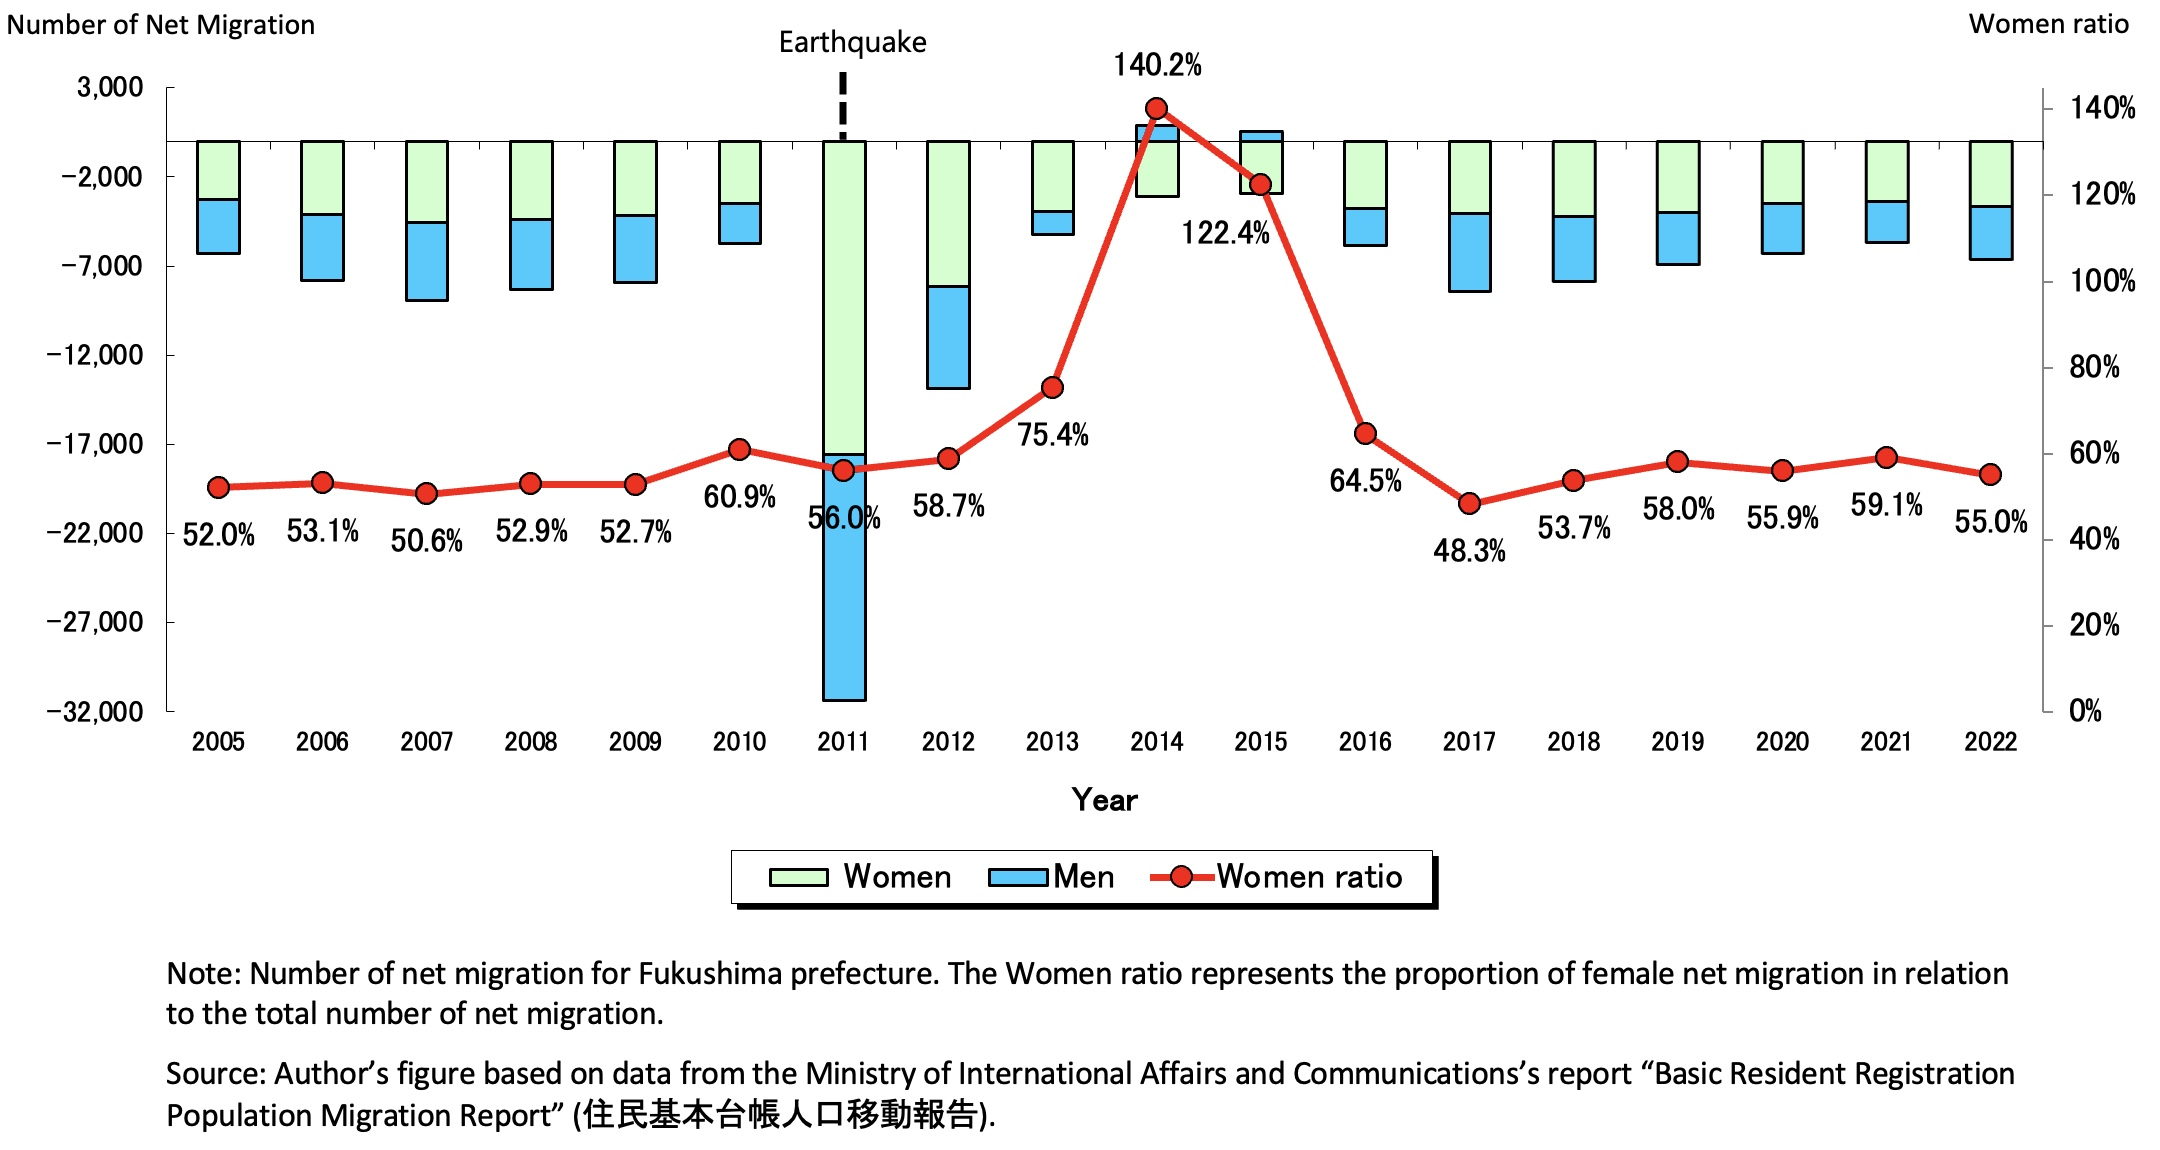
\includegraphics[width=0.70\textwidth]{Number of net migration.jpeg}  % 幅を本文の80%に設定
    \caption{The Number of Net Migration and The Proportion of Female Net Out-migration
to Total Net Out-migration in Fukushima Pref.}

\end{figure}

\vspace{-0.75cm}
\evacueeslinks

\end{frame}

%%%%%%%%%%%%%%%%%%%%%%
%%%%%%%%%%%%%%%%%
% Proportion of Employed Persons by Industry
%%%%%%%%%%%%%%%%%%%%%%%%%%

\begin{frame}[label=appendix3]
\frametitle{Proportion of Employed Persons - Fukushima Pref (2010)}

% The figure shows the proportion of employed individuals by industry and gender in Fukushima Prefecture in 2010, before the disaster. Focusing on the construction industry, the data reveals that approximately 95% of workers were male. This strong male dominance meant that when construction jobs surged after the disaster, most of the new positions were filled by men. As a result, there was little to no growth in female employment within this sector. This significant gender disparity in the construction industry explains why male employment saw a substantial rise, while female employment did not, contributing to the overall gender gap observed in employment changes.


\vspace{0.20cm} 

\returnbutton{numbers_of_workers}{Return}  % 特定のスライドにリンク


\begin{figure}[!t]
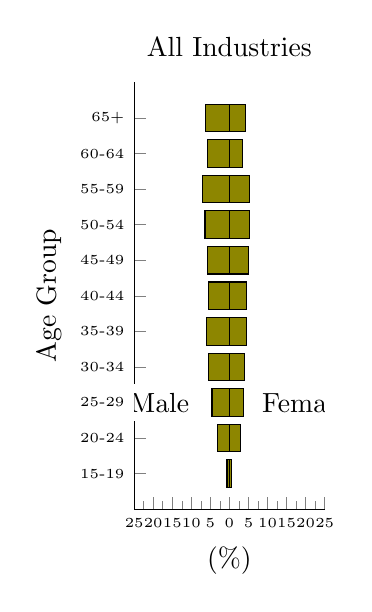
\begin{tikzpicture}
\begin{axis}[
    width=0.33\textwidth,
    height=7cm,
    xbar stacked,
    xmin=-25,
    xmax=25,
    xtick={-25, -20, -15, -10, -5, 0, 5, 10, 15, 20, 25},
    xticklabels={25, 20, 15, 10, 5, 0, 5, 10, 15, 20, 25},
    xlabel={(\%)},
    ylabel={Age Group},
    ytick={1,2,3,4,5,6,7,8,9,10,11},
    yticklabels={15-19, 20-24, 25-29, 30-34, 35-39, 40-44, 45-49, 50-54, 55-59, 60-64, 65+},
    title={All Industries},
    axis y line*=left,
    axis x line*=bottom,
    bar width=3.5mm,
    xticklabel style={font=\tiny},
    yticklabel style={font=\tiny},
    xlabel style={font=\normalsize},
    minor x tick num=1,
    grid style={line width=.1pt, draw=gray!20},
    major grid style={line width=.2pt,draw=gray!50},
]
\addplot[xbar, fill=olive] coordinates {(-6.2968,11) (-5.7348,10) (-7.0630,9) (-6.4160,8) (-5.8457,7) (-5.4109,6) (-6.0469,5) (-5.5079,4) (-4.5710,3) (-3.1366,2) (-0.6502,1)};
\addplot[xbar, fill=olive] coordinates {(4.1861,11) (3.5393,10) (5.1758,9) (5.2826,8) (4.9579,7) (4.4568,6) (4.5115,5) (4.0165,4) (3.6677,3) (2.9304,2) (0.5957,1)};
\node[anchor=east, fill=white] at (axis cs:-8,3) {Male};
\node[anchor=west, fill=white] at (axis cs:6,3) {Female};
\end{axis}
\end{tikzpicture}
\hfill
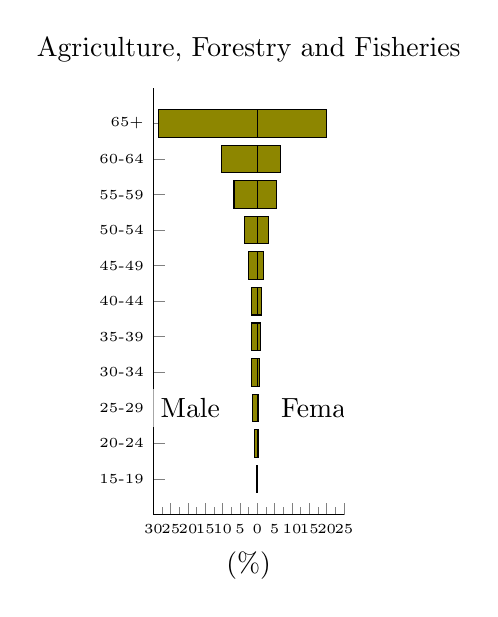
\begin{tikzpicture}
\begin{axis}[
    width=0.33\textwidth,
    height=7cm,
    xbar stacked,
    xmin=-30,
    xmax=25,
    xtick={-30, -25, -20, -15, -10, -5, 0, 5, 10, 15, 20, 25},
    xticklabels={30, 25, 20, 15, 10, 5, 0, 5, 10, 15, 20, 25},
    xlabel={(\%)},
    ytick={1,2,3,4,5,6,7,8,9,10,11},
    yticklabels={15-19, 20-24, 25-29, 30-34, 35-39, 40-44, 45-49, 50-54, 55-59, 60-64, 65+},
    yticklabel pos=right,
    title={Agriculture, Forestry and Fisheries},
    axis y line*=left,
    axis x line*=bottom,
    bar width=3.5mm,
    xticklabel style={font=\tiny},
    yticklabel style={font=\tiny},
    xlabel style={font=\normalsize},
    minor x tick num=1,
    grid style={line width=.1pt, draw=gray!20},
    major grid style={line width=.2pt,draw=gray!50},
]
\addplot[xbar, fill=olive] coordinates {(-28.5896,11) (-10.3951,10) (-6.7607,9) (-3.8248,8) (-2.5634,7) (-1.6352,6) (-1.6058,5) (-1.6520,4) (-1.2908,3) (-0.8218,2) (-0.1694,1)};
\addplot[xbar, fill=olive] coordinates {(20.0734,11) (6.5899,10) (5.5664,9) (3.2718,8) (1.7640,7) (1.1144,6) (0.8792,5) (0.6888,4) (0.4494,3) (0.2394,2) (0.0546,1)};
\node[anchor=east, fill=white] at (axis cs:-8,3) {Male};
\node[anchor=west, fill=white] at (axis cs:4,3) {Female};
\end{axis}
\end{tikzpicture}
\hfill
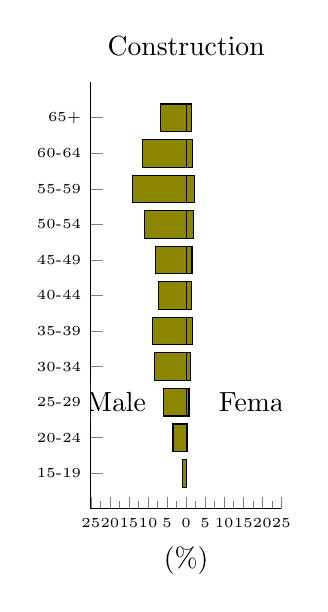
\begin{tikzpicture}
\begin{axis}[
    width=0.33\textwidth,
    height=7cm,
    xbar stacked,
    xmin=-25,
    xmax=25,
    xtick={-25, -20, -15, -10, -5, 0, 5, 10, 15, 20, 25},
    xticklabels={25, 20, 15, 10, 5, 0, 5, 10, 15, 20, 25},
    xlabel={(\%)},
    ytick={1,2,3,4,5,6,7,8,9,10,11},
    yticklabels={15-19, 20-24, 25-29, 30-34, 35-39, 40-44, 45-49, 50-54, 55-59, 60-64, 65+},
    yticklabel pos=right,
    title={Construction},
    axis y line*=left,
    axis x line*=bottom,
    bar width=3.5mm,
    xticklabel style={font=\tiny},
    yticklabel style={font=\tiny},
    xlabel style={font=\normalsize},
    minor x tick num=1,
    grid style={line width=.1pt, draw=gray!20},
    major grid style={line width=.2pt,draw=gray!50},
]
\addplot[xbar, fill=olive] coordinates {(-6.6875,11) (-11.4525,10) (-14.1118,9) (-10.9621,8) (-8.1361,7) (-7.1541,6) (-8.9182,5) (-8.3385,4) (-6.0411,3) (-3.4449,2) (-0.8749,1)};
\addplot[xbar, fill=olive] coordinates {(1.2939,11) (1.7058,10) (2.1069,9) (1.8165,8) (1.5332,7) (1.4439,6) (1.6165,5) (1.2035,4) (0.7380,3) (0.3726,2) (0.0476,1)};
\node[anchor=east, fill=white] at (axis cs:-8,3) {Male};
\node[anchor=west, fill=white] at (axis cs:6,3) {Female};
\end{axis}
\end{tikzpicture}

\caption{Proportion of Employed Persons Aged 15 and Over by Industry, Age (5-year groups), and Sex - Fukushima Pref. (2010)}
\label{fig:fukushima_Proportion_Employed}
\end{figure}

\end{frame}

%%%%%%%%%%%%%%%%%%%%%%%%%%%%%%%%
\begin{frame}{Methodology and Empirical Strategy for Further Research: TWEF Event Study with a Triple Difference Estimator}
    \begin{itemize}
    \item Two-Way Fixed Effects (TWFE) Event Study approach with a triple difference estimator, incorporating gender differences and including both individual fixed effects and time fixed effects:

\begin{equation}
Y_{ipgt} = \beta_i + \eta_t + \sum_{l \in L} (\delta_l\ + \gamma_l \cdot Female_i) \cdot 1[t-s = l] +  \mathbf \gamma {X}_{ipgt}+\epsilon_{ipgt}
\end{equation}
\end{itemize}

\end{frame}
%%%%%%%%%%%%%%%%%%%%%%%%%%%%%%%%

%%%%%%%%%%%%%%%%%%%%%%%%%%%%%%%%

\begin{frame}

Basic DID analysis (JHPS-CPS)

\vspace{-0.3cm}

\begin{table}[htbp]
\centering
\caption{DID Estimates of Disaster Impact on Monthly Income}

\scalefont{0.65}
\begin{tabular}{@{}l*{6}{c}@{}}
          &\multicolumn{3}{c}{Male}                                &\multicolumn{3}{c}{Female}                              \\\cmidrule(lr){2-4}\cmidrule(lr){5-7}
          &\multicolumn{1}{c}{(1)}&\multicolumn{1}{c}{(2)}&\multicolumn{1}{c}{(3)}&\multicolumn{1}{c}{(4)}&\multicolumn{1}{c}{(5)}&\multicolumn{1}{c}{(6)}\\
          &\multicolumn{1}{c}{Basic}&\multicolumn{1}{c}{Education}&\multicolumn{1}{c}{Edu+Occ}&\multicolumn{1}{c}{Basic}&\multicolumn{1}{c}{Education}&\multicolumn{1}{c}{Edu+Occ}\\
\toprule
Disaster Impact (DID)&   -0.841         &   -0.835         &   -1.444         &    0.633         &    0.575         &    1.114\sym{***}\\
          &  (1.151)         &  (1.132)         &  (1.204)         &  (0.521)         &  (0.493)         &  (0.238)         \\
\addlinespace
Post-Disaster Period&   -1.083\sym{***}&   -1.055\sym{***}&   -0.844\sym{**} &    0.148         &    0.159         &    0.033         \\
          &  (0.315)         &  (0.317)         &  (0.325)         &  (0.263)         &  (0.265)         &  (0.282)         \\
\addlinespace
Age       &    2.875\sym{***}&    2.842\sym{***}&    2.397\sym{***}&    1.414\sym{***}&    1.413\sym{***}&    1.030\sym{***}\\
          &  (0.209)         &  (0.215)         &  (0.196)         &  (0.189)         &  (0.180)         &  (0.167)         \\
\addlinespace
Age Squared&   -0.029\sym{***}&   -0.029\sym{***}&   -0.024\sym{***}&   -0.013\sym{***}&   -0.013\sym{***}&   -0.009\sym{***}\\
          &  (0.002)         &  (0.002)         &  (0.002)         &  (0.002)         &  (0.002)         &  (0.001)         \\
\midrule
Education &       No         &      Yes         &      Yes         &       No         &      Yes         &      Yes         \\
Occupation&       No         &       No         &      Yes         &       No         &       No         &      Yes         \\
$\textit{N}$&   11,419         &   11,313         &   10,986         &   10,493         &   10,407         &   10,055         \\
$\textit{Adjusted R}^2$&    0.759         &    0.760         &    0.772         &    0.620         &    0.620         &    0.635         \\
\bottomrule
\end{tabular}

\\\\{\linewidth}{\tiny Standard errors clustered at prefecture level in parentheses}\\\\
\\\\{\linewidth}{\tiny $*p<0.1$, $**p<0.05$, $***p<0.01$}\\\\


\label{table:basic_DID_Monthly_income}

\end{table}

\end{frame}

%%%%%%%%%%%%%%%%%%%%%%%%%%%%%%%%

\begin{frame}


Results of the TWFE Event Study

\vspace{-0.3cm}

%******************************************
%* TWFE Event Study: Impact of Disaster on Monthly Income: Female
%******************************************

\begin{table}[htbp]
\centering
\caption{Effects of Disaster on Monthly Income of Females in Disaster-Affected Prefectures}

\vspace{-0.1cm}

\scalefont{0.350}

\begin{tabular}{@{\extracolsep{5pt}}lccccc}
            &\multicolumn{1}{c}{(1)}&\multicolumn{1}{c}{(2)}&\multicolumn{1}{c}{(3)}&\multicolumn{1}{c}{(4)}&\multicolumn{1}{c}{(5)}\\
            &\multicolumn{1}{c}{OLS Basic Model}&\multicolumn{1}{c}{OLS Age Control}&\multicolumn{1}{c}{OLS Full Model}&\multicolumn{1}{c}{IPW ATE}&\multicolumn{1}{c}{IPW ATT}\\
\midrule
2 years before (Year 2009)&       1.805         &       1.498         &       0.529         &       1.261         &       1.359         \\
            &     (1.547)         &     (1.523)         &     (2.042)         &     (1.929)         &     (1.955)         \\
\addlinespace
1 year before (Year 2010)&       0.085         &      -0.137         &      -0.797         &      -0.866         &      -0.731         \\
            &     (1.220)         &     (1.196)         &     (1.253)         &     (0.956)         &     (1.248)         \\
\addlinespace
Baseline, 2 months before (Year 2011)&       0.000         &       0.000         &       0.000         &       0.000         &       0.000         \\
            &         (.)         &         (.)         &         (.)         &         (.)         &         (.)         \\
\addlinespace
1 year after (Year 2012)&       1.180         &       1.242         &       2.093\sym{*}  &       2.305\sym{*}  &       2.476\sym{*}  \\
            &     (1.300)         &     (1.319)         &     (1.209)         &     (1.307)         &     (1.316)         \\
\addlinespace
2 years after (Year 2013)&       0.497         &       0.804         &       1.470         &       1.665         &       1.999         \\
            &     (2.047)         &     (2.000)         &     (1.875)         &     (2.242)         &     (2.230)         \\
\addlinespace
5 years after (Year 2016)&       3.823         &       5.023\sym{*}  &       5.907\sym{**} &       5.803\sym{**} &       5.900\sym{**} \\
            &     (2.726)         &     (2.930)         &     (2.367)         &     (2.554)         &     (2.456)         \\
\addlinespace
6 years after (Year 2017)&      -0.320         &       0.909         &       1.391         &       0.641         &       1.663         \\
            &     (3.121)         &     (3.365)         &     (3.649)         &     (4.624)         &     (3.967)         \\
\addlinespace
7 years after (Year 2018)&       2.888         &       4.448\sym{*}  &       4.074\sym{*}  &       3.771\sym{*}  &       3.754         \\
            &     (2.330)         &     (2.376)         &     (2.070)         &     (2.159)         &     (2.484)         \\
\addlinespace
Age         &                     &       2.347\sym{***}&       1.976\sym{***}&       1.238\sym{*}  &       1.461\sym{*}  \\
            &                     &     (0.324)         &     (0.281)         &     (0.651)         &     (0.779)         \\
\addlinespace
Age Squared &                     &      -0.022\sym{***}&      -0.018\sym{***}&      -0.016\sym{***}&      -0.016\sym{***}\\
            &                     &     (0.001)         &     (0.001)         &     (0.002)         &     (0.003)         \\
\midrule
Education   &          No         &          No         &         Yes         &         Yes         &         Yes         \\
Occupation  &          No         &          No         &         Yes         &         Yes         &         Yes         \\
$\textit{N}$&      21,912         &      21,912         &      21,041         &      20,569         &      20,569         \\
$\textit{Adjusted R}^2$&       0.776         &       0.783         &       0.795         &       0.762         &       0.739         \\
\bottomrule
\multicolumn{6}{l}{\tiny Standard errors in parentheses}\\
\multicolumn{6}{l}{\tiny \sym{*} \(p<0.1\), \sym{**} \(p<0.05\), \sym{***} \(p<0.01\)}\\


\end{tabular}

\label{table:Monthly_Income}

\end{table}

\end{frame}

%%%%%%%%%%%%%%%%%%%%%%%%%%%%%%%%

\begin{frame}

\begin{figure}[h!]
    \centering
    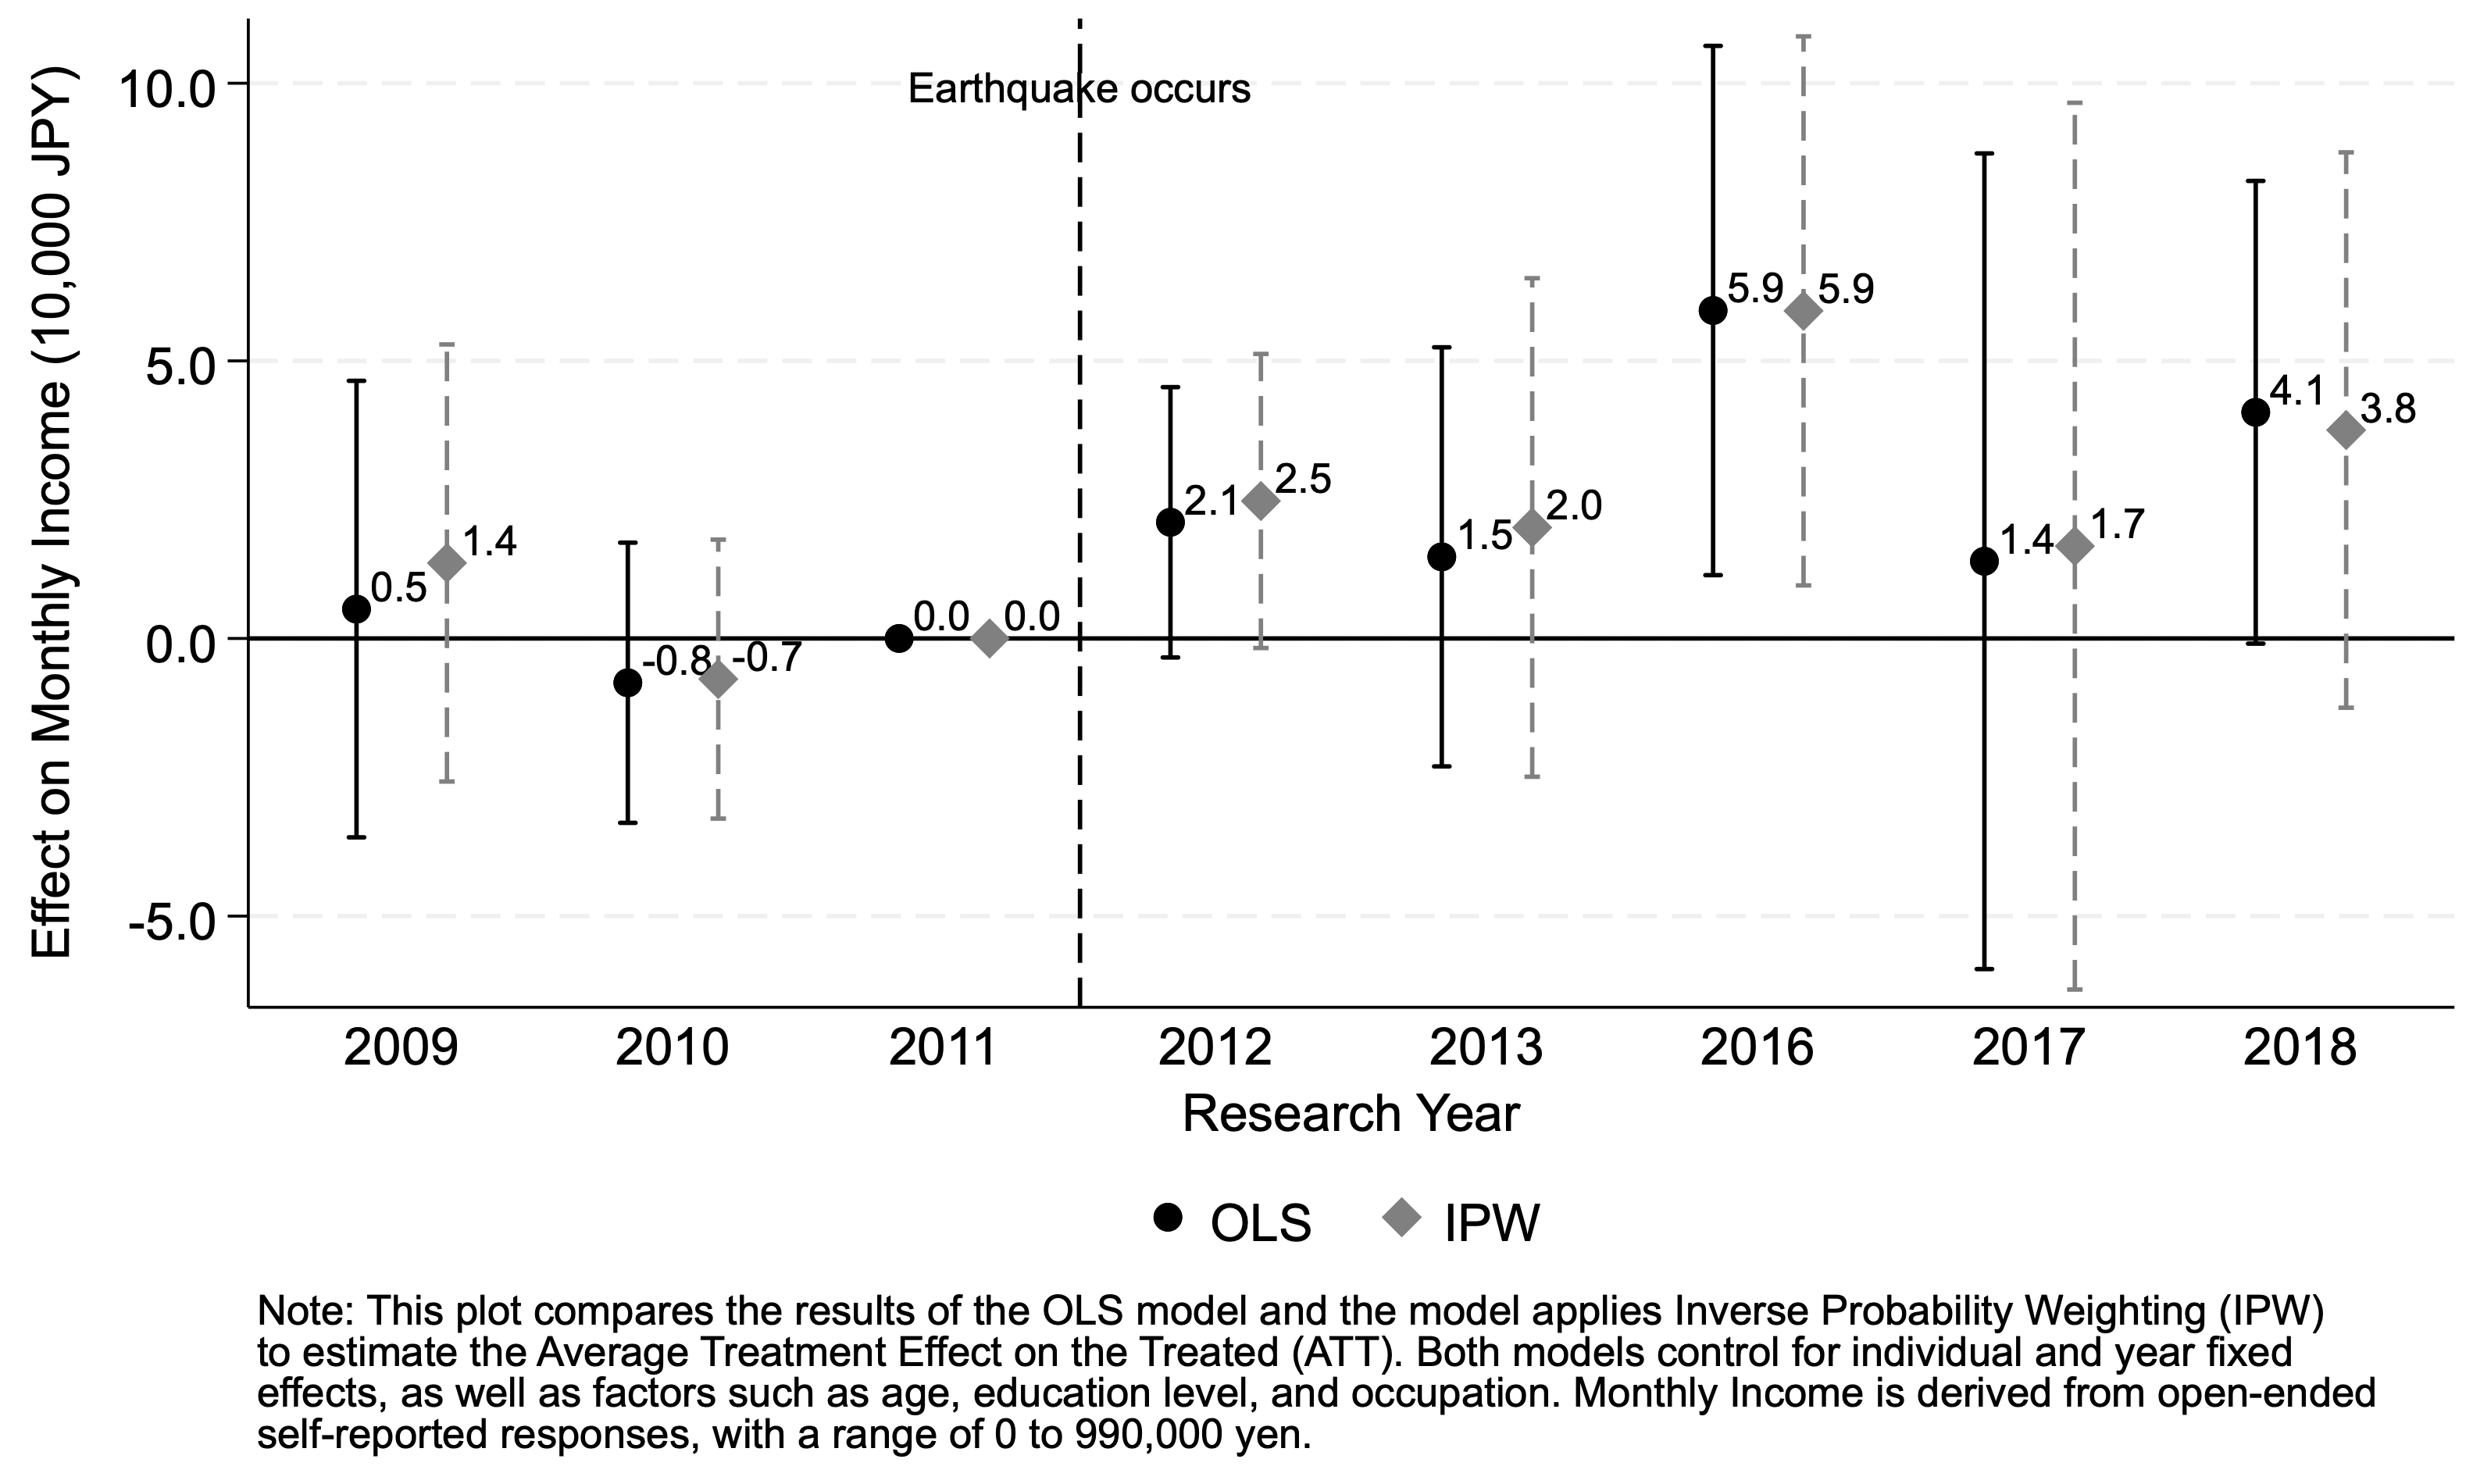
\includegraphics[width=0.70\textwidth]{monthly_income_comparison.png}  % 幅を本文の80%に設定
    \caption{TWFE Event Study: Effects on Females in Disaster-Affected Prefectures}

\end{figure}

\end{frame}

%%%%%%%%%%%%%%%%%%%%%%%%%%%%%%%%

%---------------------------------------
% Slide: Fishery in Fukushima
%---------------------------------------


\begin{frame}[label=image]
\frametitle{Types of Employment in Fukushima's Fisheries}

\vspace{0.2cm}

\returnbutton{conclusion}{Return}


    \vspace{-0.2cm}
  \begin{figure}
    \centering
    \includegraphics[width=0.93\textwidth]{Fishery-1.0.pdf}

  \end{figure}
\end{frame}


%%%%%%%%%%%%%%%%%%%%%%%%%%%%%%%%
% Labour Force Participation Rates
%%%%%%%%%%%%%%%%%%%%%%%%%%%%%%%%


\begin{frame}[label=LFP]
    \frametitle{Labor Force Participation Rates by Age and Gender - Fukushima Pref}

    \vspace{0.25cm}

    \returnbutton{conclusion}{Return}

    \vspace{-0.4cm}

    \begin{figure}
        \centering

        \begin{subfigure}{\textwidth}
            \centering
            \begin{minipage}{0.48\textwidth}
                \centering
                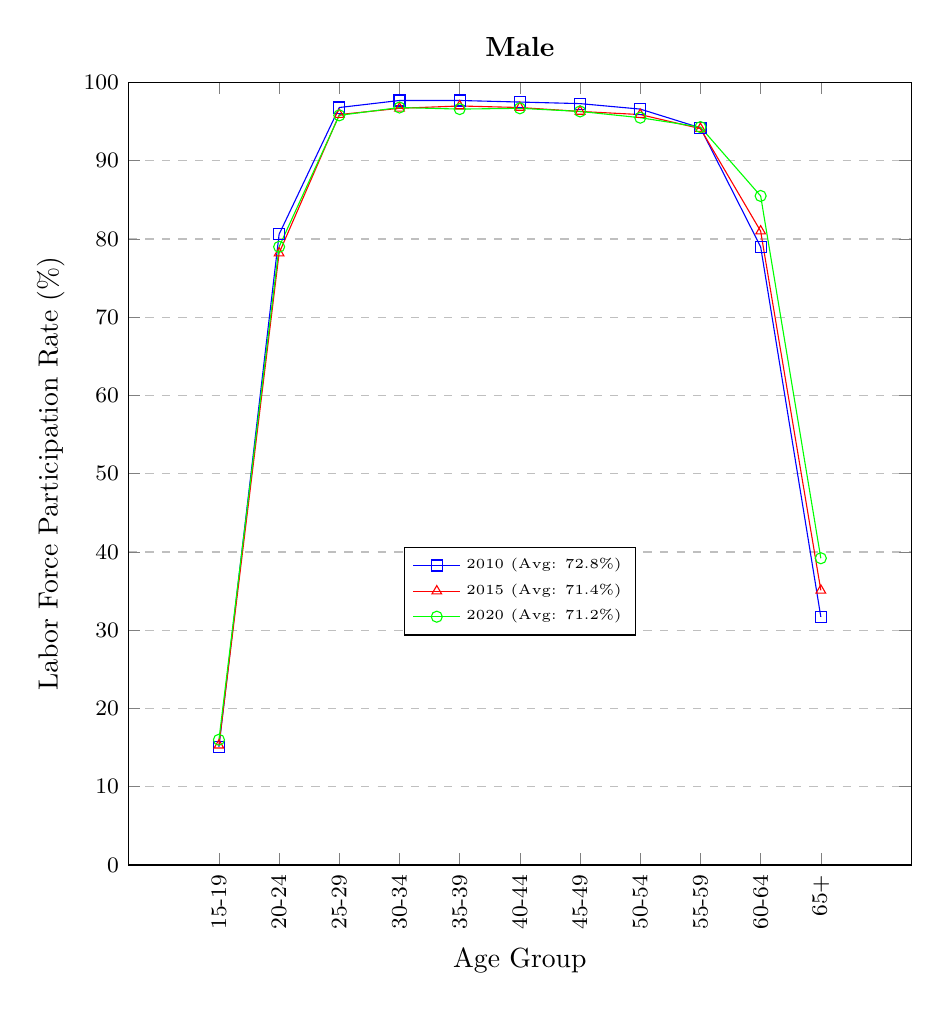
\begin{tikzpicture}
                \begin{axis}[
                    title={\textbf{Male}},
                    xlabel={Age Group},
                    ylabel={Labor Force Participation Rate (\%)},
                    xmin=0, xmax=12,
                    ymin=0, ymax=100,
                    xtick={1,2,3,4,5,6,7,8,9,10,11},
                    xticklabels={15-19,20-24,25-29,30-34,35-39,40-44,45-49,50-54,55-59,60-64,65+},
                    x tick label style={rotate=90,anchor=east,font=\footnotesize},
                    y tick label style={font=\footnotesize},
                    legend style={font=\tiny, at={(0.5,0.35)}, anchor=center, legend columns=1},
                    ymajorgrids=true,
                    grid style=dashed,
                    enlarge x limits={abs=0.5},
                    width=0.95\linewidth,
                    height=0.95\linewidth,
                ]

                \addplot[color=blue, mark=square] coordinates {
                    (1,15.1)(2,80.6)(3,96.8)(4,97.7)(5,97.7)(6,97.5)(7,97.3)(8,96.6)(9,94.2)(10,79.0)(11,31.7)
                };

                \addplot[color=red, mark=triangle] coordinates {
                    (1,15.3)(2,78.2)(3,95.9)(4,96.7)(5,97.0)(6,96.8)(7,96.3)(8,95.9)(9,94.1)(10,81.0)(11,35.1)
                };

                \addplot[color=green, mark=o] coordinates {
                    (1,16.0)(2,79.0)(3,95.8)(4,96.8)(5,96.6)(6,96.7)(7,96.3)(8,95.5)(9,94.3)(10,85.5)(11,39.2)
                };

                \legend{
                    2010 (Avg: 72.8\%),
                    2015 (Avg: 71.4\%),
                    2020 (Avg: 71.2\%)
                }
                \end{axis}
                \end{tikzpicture}
            \end{minipage}
            \hfill
            \begin{minipage}{0.48\textwidth}
                \centering
                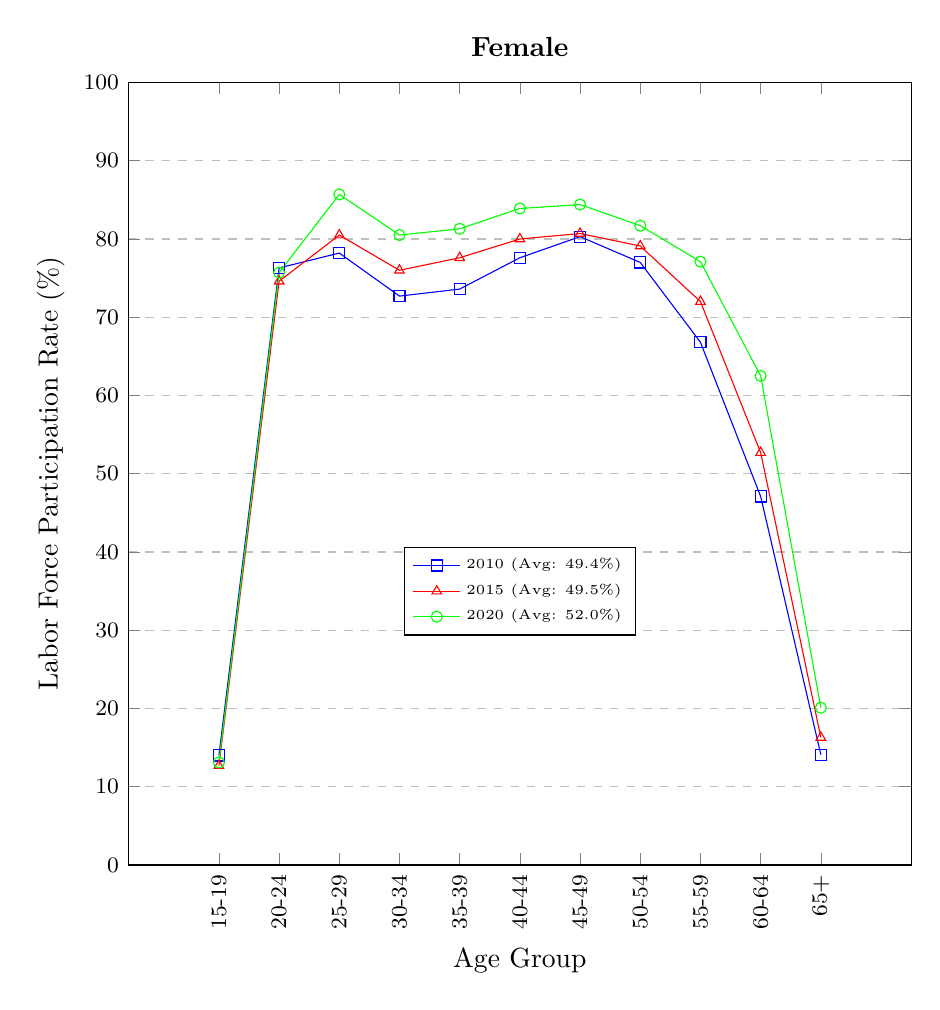
\begin{tikzpicture}
                \begin{axis}[
                    title={\textbf{Female}},
                    xlabel={Age Group},
                    ylabel={Labor Force Participation Rate (\%)},
                    xmin=0, xmax=12,
                    ymin=0, ymax=100,
                    xtick={1,2,3,4,5,6,7,8,9,10,11},
                    xticklabels={15-19,20-24,25-29,30-34,35-39,40-44,45-49,50-54,55-59,60-64,65+},
                    x tick label style={rotate=90,anchor=east,font=\footnotesize},
                    y tick label style={font=\footnotesize},
                    legend style={font=\tiny, at={(0.5,0.35)}, anchor=center, legend columns=1},
                    ymajorgrids=true,
                    grid style=dashed,
                    enlarge x limits={abs=0.5},
                    width=0.95\linewidth,
                    height=0.95\linewidth,
                ]

                \addplot[color=blue, mark=square] coordinates {
                    (1,14.0)(2,76.3)(3,78.2)(4,72.7)(5,73.6)(6,77.6)(7,80.3)(8,77.0)(9,66.8)(10,47.1)(11,14.1)
                };

                \addplot[color=red, mark=triangle] coordinates {
                    (1,12.7)(2,74.6)(3,80.5)(4,76.0)(5,77.6)(6,80.0)(7,80.7)(8,79.1)(9,72.0)(10,52.7)(11,16.3)
                };

                \addplot[color=green, mark=o] coordinates {
                    (1,13.1)(2,75.7)(3,85.7)(4,80.5)(5,81.3)(6,83.9)(7,84.4)(8,81.7)(9,77.1)(10,62.5)(11,20.1)
                };

                \legend{
                    2010 (Avg: 49.4\%),
                    2015 (Avg: 49.5\%),
                    2020 (Avg: 52.0\%)
                }
                \end{axis}
                \end{tikzpicture}
            \end{minipage}
        \end{subfigure}

    \end{figure}

\end{frame}


%---------------------------------------
% Slide: DID
%---------------------------------------


\begin{frame}[label=did]

\vspace{0.5cm}

\returnbutton{conclusion}{Return}

    \vspace{-0.3cm}
  \begin{figure}
    \centering
    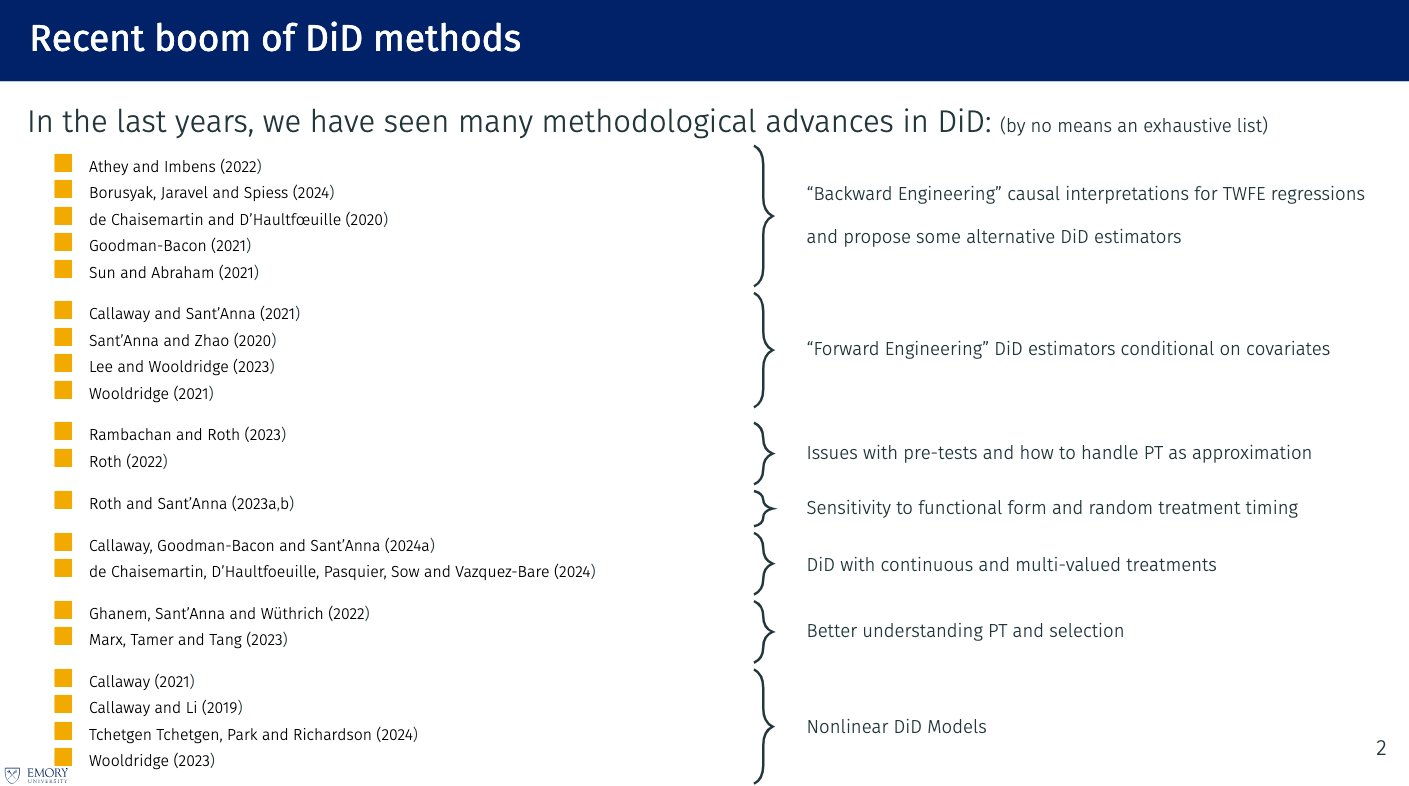
\includegraphics[width=0.93\textwidth]{DID.JPG}

  \end{figure}
\end{frame}

%%%%%%%%%%%%%%%%%%%%%%%%%%%%%%%%
%\section{References}

\begin{frame}[allowframebreaks]
    \frametitle{References}
    \small % 文字サイズを小さくして、より多くの参考文献を1ページに収める
    \bibliographystyle{apacite} % APAスタイルを使用
    \bibliography{references}
    % \nocite{*} コマンドを削除
\end{frame}


%%%%%%%%%%%%%%%%%%%%%%%%%%%%%%%%





\end{document}